\documentclass[a4paper,12pt]{report}
\usepackage[catalan]{varioref}
\usepackage{setspace}
\usepackage[margin=2.54cm]{geometry}
\usepackage{pdfpages}
\usepackage[utf8]{inputenc}
\usepackage[catalan]{babel}
\usepackage{graphicx,subcaption}
\usepackage{graphics}
\usepackage{lscape}
\usepackage{pdflscape}
\usepackage{float}
\usepackage{textcomp}
\usepackage{amsmath}
\usepackage{hyperref}
\usepackage{subcaption}
\usepackage{pgfplots}
\usepackage{tikz}
\usepackage{fancyvrb}
\usepackage{parskip}
\usepackage{changepage}
\usepackage{enumitem}
\usepackage{tcolorbox}
\usepackage[all]{hypcap}
\usepackage{xcolor}
\usepackage{listings}
\definecolor{green}{HTML}{228B22}
\definecolor{orange}{HTML}{FFC107}
\usepackage{color}
\definecolor{dkgreen}{rgb}{0,0.6,0}
\definecolor{gray}{rgb}{0.5,0.5,0.5}
\definecolor{mauve}{rgb}{0.58,0,0.82}
\lstset{escapeinside={<@}{@>}}

\hypersetup{
    colorlinks,
    citecolor=black,
    filecolor=black,
    linkcolor=black,
    urlcolor=blue
}


\lstset{frame=tb,
    language=python,
    aboveskip=3mm,
    belowskip=3mm,
    showstringspaces=false,
    columns=flexible,
    basicstyle={\small\ttfamily},
    numbers=none,
    numberstyle=\tiny\color{gray},
    keywordstyle=\color{blue},
    commentstyle=\color{dkgreen},
    stringstyle=\color{mauve},
    breaklines=true,
    breakatwhitespace=true, tabsize=3
}
\onehalfspacing

\begin{document}
\thispagestyle{empty}
\pagenumbering{gobble}
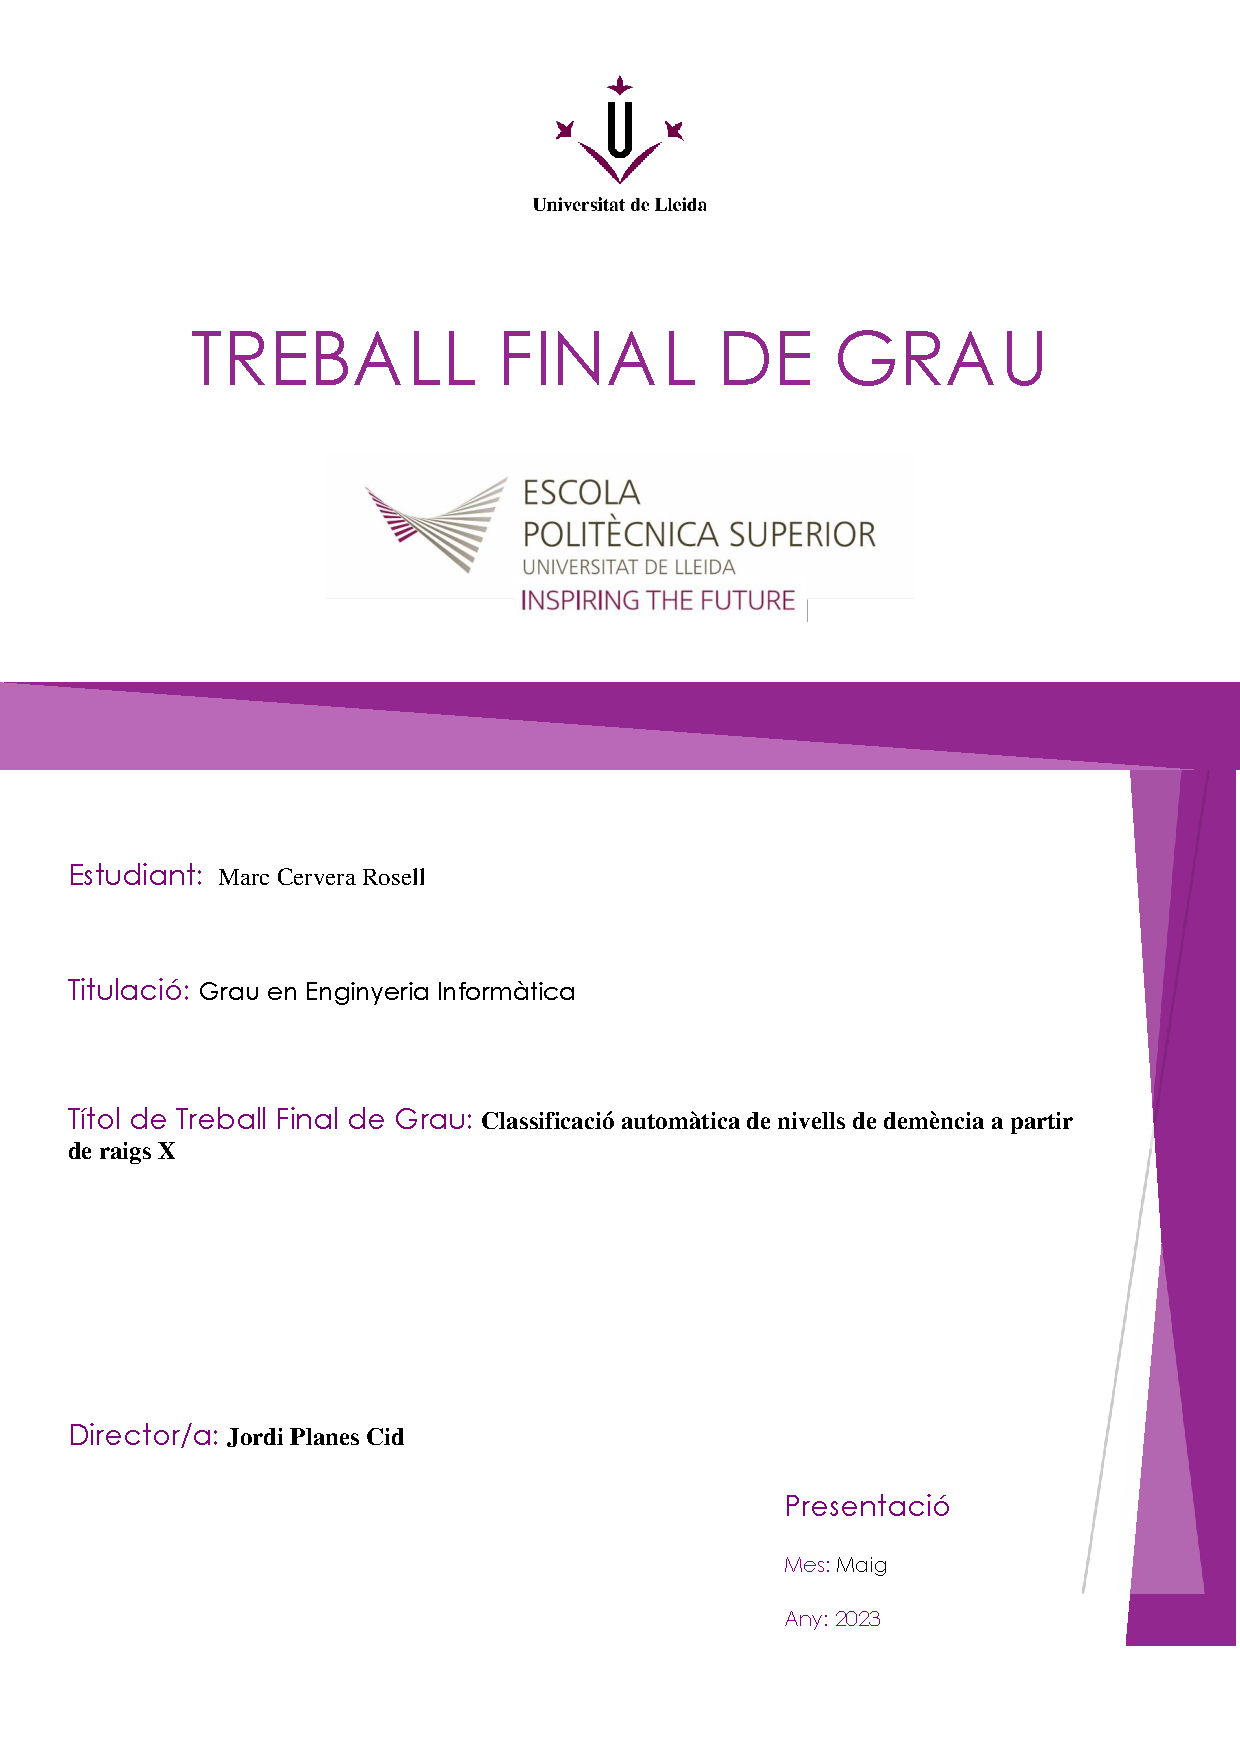
\includepdf{Portada-TFG}
\thispagestyle{empty}
\tableofcontents
\thispagestyle{empty}
\listoffigures
\thispagestyle{empty}
\listoftables
\thispagestyle{empty}
\newpage
\pagenumbering{arabic}
\chapter*{Introducció}
\addcontentsline{toc}{chapter}{Introducció}
Detectar de manera precoç l'Alzheimer en una persona és un dels desafiaments que enfronta la medicina del segle XXI. Els mètodes utilitzats avui dia per a la detecció precoç d'aquesta malaltia són molt costosos i requereixen una copiosa inversió de temps i recursos. Tot i que la detecció d'aquesta afecció és un desafiament realment complicat, és crucial per poder garantir un tractament i una qualitat de vida adequats per als pacients que, per desgràcia, pateixen els efectes d'aquesta malura.\\
Durant la realització d'aquest treball de final de grau, s'investigarà de quina manera pot ajudar la intel·ligència artificial en la detecció primerenca de la malaltia d'Alzheimer a partir d'imatges de ressonància magnètica cerebral (MRI en anglès). L'aplicació del \textit{Machine Learning} en el camp de la salut, i més concretament en el cas que tracta aquest treball (l'Alzheimer), és una tècnica que augura moltes esperances de facilitar la detecció precoç d'aquesta terrible malaltia. Les esperances es basen en el fet que l'ús de la intel·ligència artificial pot ajudar, com s'ha esmentat, a detectar de manera primerenca aquesta malaltia d'una manera no invasiva ni dolorosa per al pacient, cosa que podria millorar molt significativament la qualitat de vida i reduir els costos que suposa el diagnòstic tardà i el tractament.\\
Com s'explicarà més endavant en aquest document, les xarxes neuronals convolucionals, s'han convertit en la tècnica que proporciona més esperances a les comunitats científica i sanitària, perquè són capaces d'extreure les característiques complexes d'una ressonància magnètica i utilitzar-les per ajudar al professional mèdic corresponent a confirmar o descartar el diagnòstic d'Alzheimer.\\
Per dur a terme l'objectiu principal d'aquest treball de final de grau, es farà ús de la tècnica d'aprenentatge supervisat, per entrenar una sèrie de dades etiquetades que “ensenyaran” a la xarxa convolucional a diferenciar entre quatre nivells possibles de demència per Alzheimer. Aquests quatre nivells són; no dement, dement molt lleu, dement lleu, dement moderat.\\
L'estructura que seguirà el treball consta de vuit blocs, el primer dels quals contindrà informació sobre la malaltia d'Alzheimer. El segon, conformarà el bloc del marc teòric computacional, en el qual constarà informació detallada sobre la tecnologia emprada en la realització del treball. El tercer bloc tractarà sobre les aplicacions de la intel·ligència artificial en el camp de la salut. Concretament, es comentaran diversos aspectes relacionats amb l'aplicació de la tecnologia per al diagnòstic i tractament de la malaltia. El següent bloc contindrà informació sobre el desenvolupament de la proposta, tot mostrant anàlisis gràfiques de les mètriques de rendiment de la xarxa neuronal com una anàlisi exhaustiva d'en quines parts de les imatges es fixa el model en el moment de fer la classificació de la imatge d'input. Seguidament, el cinquè bloc contindrà les conclusions extretes després de realitzar la investigació. El sisè bloc contindrà els glossaris del treball on es definiran alguns conceptes que no hagin pogut quedar clars en el moment de la redacció d'aquest document. En el penúltim bloc, constaran els agraïments a les persones que han fet possible la realització i la finalització exitosa d'aquest treball. Finalment, el vuitè i últim bloc, especificarà les referències bibliogràfiques que han estat necessàries per a la recerca.
\chapter*{\textit{Abstract}}
\addcontentsline{toc}{chapter}{Abstract}
\textit{This document will explain the development process of an artificial intelligence model able to identify up to four levels of dementia caused by Alzheimer's disease. These levels are; “non-demented”, “ver mild demented”, “mild demented” and “moderate demented”.\\
The main aim of this thesis is to give to the health workers a new tool to get helped to confirm or discart the Alzheimer's diagnosis, but the most important is not to give a diagnosis tool. The most essential, is to give a new tool that allows early diagnosis to give to the patients the best life quality and reduce the costs of late diagnosis.}
\chapter*{Marc teòric clínic}
\addcontentsline{toc}{chapter}{Marc teòric clínic}
\section*{Quan i qui va descobrir l'Alzheimer?}
\addcontentsline{toc}{section}{Quan i qui va descobrir l'Alzheimer?}
Abans d'entrar de ple en què és l'Alzheimer, quins símptomes presenta, etc. cal fer una mica la vista enrere a la història per saber qui i quan va descobrir aquesta malaltia.\\
A principis del segle XX, concretament l'any 1901, el psiquiatre alemany \textit{Alois Alzheimer}, es va topar amb uns estranys símptomes en una pacient anomenada \textit{Auguste Deter} de cinquanta-un anys. Aquesta dona patia pèrdua de memòria a curt termini i al·lucinacions auditives, cosa que va deixar perplex al doctor \textit{Alzheimer}. Descobrir els motius del comportament de la seva pacient, es va convertir en l'obsessió del doctor i, cinc anys després, quan la pacient \textit{Auguste Deter} va morir en un asil de la ciutat de \textit{Frankfurt}, \textit{Alzheimer} va conservar dues coses que van ser elements clau en la història d'aquesta malaltia. Els elements conservats pel doctor, varen ser l'historial clínic de la pacient i estudis del seu cervell. El Dr. \textit{Alzheimer} va portar a \textit{Munich}, concretament al laboratori d'\textit{Emil Kraepelin} un pioner en l'àrea psiquiàtrica, els seus descobriments amb la finalitat de poder començar una investigació encara més rigorosa.\\
Durant l'autòpsia del cervell de la seva pacient, el doctor \textit{Alzheimer} va descobrir que l'escorça cerebral era més estreta del normal i hi havia dos tipus d'anomalies notables: plaques d'amiloide, que són acumulacions de proteïnes entre les neurones, i cabdells d'una altra proteïna anomenada tau. Aquestes anomalies estan relacionades amb la disminució de la funció neuronal.\\
El doctor va presentar el cas de la seva pacient en una reunió de psiquiatria, però no va generar molt interès. No obstant això, l'any 1910, el Dr. \textit{Kraepelin} va començar a referir-se a aquella malaltia com la “malaltia d'Alzheimer”. El Dr. \textit{Alzheimer} no podia imaginar que aquell primer contacte amb aquella dona de cinquanta-un anys iniciaria una llarga i difícil batalla (batalla que avui dia encara continua amb investigadors a primera línia de batalla) per descobrir tots els símptomes i una cura per la causa de demència més comuna.\\
El Dr. \textit{Alois Alzheimer} va morir l'any 1915, però el seu llegat en el camp de la biomedicina encara és viu. El doctor és reconegut no solament per la seva descripció inicial d'una afecció, sinó també per ser un exemple d'investigador clínic. Va establir un estàndard per comprendre els desordres neurodegeneratius en mantenir una estreta relació amb els seus pacients i utilitzar eines científiques per explicar com els símptomes es relacionen amb els canvis físics del cervell.
\section*{Qué és l'Alzheimer i quins factors contribueixen a la seva aparició?}
\addcontentsline{toc}{section}{Qué és l'Alzheimer i quins factors contribueixen a la seva aparició?}
Atès que l'Alzheimer és la causa més comuna de demència, abans de definir res sobre la malaltia d'Alzheimer cal definir de manera clara que és la demència.\\
La demència, també coneguda com a trastorn neurocognitiu major, per definició, és un conjunt de símptomes que causen diverses infermetats. Aquests símptomes inclouen: afectacions en la memòria, afectacions en el comportament i afectacions en les habilitats socials de tal manera que dificulten les activitats quotidianes i la independència social.\\
Moltes de les infermetats que causen demència provoquen simptomatologia similar com pèrdua de la memòria i de l'orientació, comportament agressiu, problemes de parla i diverses afectacions a escala física. Cal remarcar que aquests símptomes es poden manifestar en moltes maneres, tot depenent de la persona afectada.\\
Un cop definit el terme de demència, es pot procedir a la definició d'Alzheimer.\\
L'Alzheimer és un tipus de demència que causa problemes amb la memòria, el pensament i el comportament. Els símptomes, generalment, es desenvolupen lentament i empitjoren amb el pas del temps, fins que són tan greus que interfereixen amb les tasques quotidianes. Cal remarcar que l'Alzheimer tot i ser la causa més comuna de demència no és l'única. En la següent imatge es pot observar un gràfic que de les demències més comunes:
\begin{figure}[H]
    \centering
    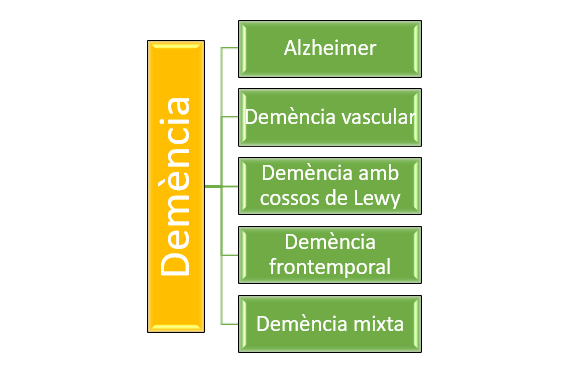
\includegraphics[scale = 0.5]{images/image_2023-03-08_172829369.png}
    \caption{Gràfic de les demències més comunes}
    \label{fig:demències}
\end{figure}
De tots els casos de demència que es diagnostiquen, s'atribueix un percentatge d'entre un 60\% i un 80\% a l'Alzheimer. En cap cas aquesta malaltia és quelcom normal de l'envelliment, tot i que el factor de risc més important sigui el pas del temps, fet que implica fer-se gran. La majoria de les persones diagnosticades amb Alzheimer són majors de seixanta-cinc anys. Tot i que, cal assenyalar que la infermetat d'Alzheimer no afecta només a persones d'avançada edat, ja que al voltant de dues-centes mil persones, solament als Estats Units, menors de seixanta-cinc anys pateixen, de manera primerenca, aquesta malaltia.\\
L'Alzheimer és una infermetat progressiva. Això significa que empitjora amb el pas del temps. En les seves primeres etapes la pèrdua de memòria és lleu, però en l'etapa final, les persones perden la capacitat de mantenir una conversa i respondre a l'entorn.\\
Tenint en compte el factor de l'edat, existeixen una totalitat de quatre factors de risc.\\
El primer factor de risc, és l'herència. La malaltia pot ser hereditària on la meitat o més de cada generació està afectada per un gen dominant. En famílies on hi ha dues generacions consecutives amb membres afectats, els fills tenen un 50\% de probabilitats de patir Alzheimer, si viuen fins als vuitanta-cinc anys. En la forma esporàdica de l'infermetat el risc no es pot determinar, però augmenta si la persona té una constitució genètica amb el gen APOE E-4. El risc solament augmenta en un 20\% sense la mutació del gen, un 47\% per aquells amb una mutació i un 91\% per aquelles persones amb dues mutacions del gen.\\
El segon factor de risc que pot contribuir a l'aparició d'Alzheimer, és un traumatisme cranial. Cal remarcar que els danys cerebrals en un pacient d'Alzheimer són majors, però el fet de patir un traumatisme cranial pot ser un factor desencadenant de la malaltia, tot i que la majoria de traumatismes cranials no són Alzheimer ni desencadenen la infermetat.
Un altre factor molt important a tenir en compte és el sexe. Com es veurà en la posteriorment a la secció d'estadístiques d'afectats per la infermetat, les dones són molt més propenses a tenir Alzheimer que els homes. De fet, s'estima només a Espanya, que en el 69\% dels casos d'Alzheimer el sexe afectat, és el sexe femení.\\
Com s'ha comentat anteriorment, els anys de vida és el factor més influent, però aquest deixa de ser un element dominant a partir dels noranta anys. A partir d'aquesta edat, el risc de patir Alzheimer disminueix, normalment. És capital posar en rellevància que, en cap cas, el nivell educatiu o intel·lectual, l'exposició continuada a l'alumini, els virus lents, les infeccions o viure en una zona rural o urbana són considerats factors de risc.
\section*{Quina simptomatologia ens ha de posar en alerta?}
\addcontentsline{toc}{section}{Quina simptomatologia ens ha de posar en alerta?}
Cent vint-i-dos anys després del descobriment de l'infermetat d'Alzheimer, per part del Dr. \textit{Alois Alzheimer}, la batalla per descobrir tots els símptomes de la malaltia continua. Avui en dia, encara no es coneix tota la simptomatologia que presenta la malaltia d'Alzheimer, però sí que hi ha determinats signes que han de posar en alerta a una persona i als seus familiars i amics.\\
Ara per ara, estan establerts deu símptomes que són senyals d'alarma per una possible demència per Alzheimer.\\
\textbf{La primera alarma és la pèrdua de memòria}. Especialment en els primers estadis de la infermetat, un dels principals senyals és oblidar informació recent, oblidar dates o esdeveniments importants, demanar la mateixa informació de manera reiterada, etc.\\
\textbf{El segon senyal d'alarma és la dificultat per planificar o resoldre problemes}. Algunes persones poden experimentar problemes per desenvolupar i seguir una rutina, treballar amb nombres seguir una recepta de cuina, concentrar-se en una tasca, etc.\\
\textbf{Com a tercera alarma, hi ha la dificultat per desenvolupar tasques habituals ja sigui a casa, a la feina o al temps d'oci}. Per exemple, es pot tenir dificultat per tasques tan usuals com rentar-se la cara, arribar d'un punt “A” a un punt “B”, sent el punt “B” una localització coneguda per la persona, administrar un pressupost o recordar les normes d'un joc.\\
\textbf{La quarta alerta és la desorientació en l'espaitemps}. Les persones amb Alzheimer obliden dates importants, les estacions de l'any i el pas del temps en general. També és molt probable que s'oblidin del lloc on es troben en aquell moment i de com han arribat allí.\\
\textbf{El cinquè senyal d'alarma és la dificultat de comprensió visual}. La comprensió visual es refereix a entendre imatges visuals i com els objectes es relacionen entre ells a l'entorn. Manca de comprensió visual també inclou la dificultat per llegir, jutjar distàncies, determinar el contrast de colors, etc.\\
\textbf{La sisena alarma és tenir impediments per utilitzar el llenguatge}. Tant en el llenguatge escrit com en la parla, les persones amb Alzheimer poden tenir dificultats per a seguir una conversa o que, per exemple, a mitja conversa parin sense tenir ni la més mínima idea del que estaven dient o que repeteixin reiteradament quelcom que acaben de dir fa escassos instants. També pot ser que no puguin trobar les paraules adients o que anomenin les coses per un nom incorrecte.\\
\textbf{L'alerta número set és col·locar objectes en llocs diferents de l'habitual i tenir dificultats per trobar-los}. Una persona afectada per la malaltia sol posar coses fora del seu lloc essent després completament incapaç de trobar-les. De vegades, és possible, que acusin altres persones de robar-los.\\
\textbf{L'antepenúltim senyal d'alarma és la disminució o la falta de judici}. La disminució de l'activitat cerebral pot provocar alteracions en la capacitat de jutjar el perill que comporta una acció i també pot provocar una alteració en la capacitat de prendre decisions.\\
\textbf{Com a penúltima alerta es troba la pèrdua d'iniciativa}. Cal subratllar, que aquest senyal és un “dels menys importants”, ja que la pèrdua d'iniciativa per participar en passatemps, activitats socials, projectes de treball o esports també es pot donar en altres malalties completament diferents de l'Alzheimer, com per exemple, la depressió.\\
\textbf{L'última alarma són els canvis d'humor o de personalitat}. Les persones amb la malaltia d'Alzheimer poden arribar a sospitar de tothom, ser persones agressives, temoroses o ansioses.
\section*{Quines fases té la malaltia?}
\addcontentsline{toc}{section}{Quines fases te la malaltia?}
En tot el món, professionals i cuidadors utilitzen l'escala de deteriorament global, desenvolupada pel Dr. Barry Reisberg, director del programa d'educació i investigació de la infermetat d'Alzheimer. Aquesta escala serveix per determinar en quin nivell de demència es troba la persona afectada d'Alzheimer.\\
Dividida en dos grans blocs; predemència (estadis 1 a 3) i demència (estadis 4 a 7), l'escala consta de set estadis clínics diferents. El punt d'inflexió on la persona ja no pot viure sense assistència continuada, és l'estadi 5.
\subsection*{Llistat d'estadis}
\addcontentsline{toc}{subsection}{Llistat d'estadis}
\begin{itemize}
    \item Bloc predemència
    \begin{itemize}
        \item Estadi 1: No demència observable.
        \item Estadi 2: Pèrdua de memòria relacionada amb l'edat.
        \item Estadi 3: Deteriorament cognitiu lleu.
    \end{itemize}
    \item Bloc de demència
    \begin{itemize}
        \item Estadi 4: Declivi cognitiu moderat. Demència lleu.
        \item Estadi 5: Declivi cognitiu moderadament sever. Demència moderada.
        \item Estadi 6: Declivi cognitiu sever. Demència moderadament severa
        \begin{itemize}
            \item Estadi 6A.
            \item Estadi 6B.
            \item Estadi 6C.
            \item Estadi 6D.
            \item Estadi 6E.
        \end{itemize}
        \item Estadi 7: Declivi cognitiu molt sever. Demència severa.
        \begin{itemize}
            \item Estadi 7A.
            \item Estadi 7B.
            \item Estadi 7C.
            \item Estadi 7D.
            \item Estadi 7E.
            \item Estadi 7F.
        \end{itemize}
    \end{itemize}
\end{itemize}
\subsection*{Característiques de cada estadi}
\addcontentsline{toc}{subsection}{Característiques de cada estadi}
\textbf{\underline{Estadi 1}:}\\
Aquest primer estadi on no es pot observar cap mena de demència és l'estadi que es dona a qualsevol edat i és l'estadi en el qual no es presenta cap símptoma de demència. Aquest és l'anomenat estadi de normalitat.\\
\textbf{\underline{Estadi 2}:}\\
El segon estadi, és l'estadi de les pèrdues de memòria relacionades amb l'edat. Les persones de seixanta-cinc anys o més asseguren tenir dificultats cognitives i/o funcionals. Aquestes dificultats inclouen recordar, com ho feien abans, els noms, dates, on han posat un determinat objecte, etc. En el món de la investigació clínica, s'han proposat molts noms per denominar aquesta fase, però el més acceptat és el deteriorament cognitiu subjectiu. Com s'ha demostrat, científicament, que els símptomes d'aquest estadi no són notables per observadors externs, per tant, aquest segon estadi són el que s'anomena “coses de l'edat”. Si la demència ha de continuar avançant, ho farà en un període d'aproximadament quinze anys.\\
\textbf{\underline{Estadi 3}:}\\
Aquesta etapa de la malaltia, anomenada deteriorament cognitiu lleu (MCI), es caracteritza per tenir dificultats subtils en la memòria i altres habilitats mentals, que són detectades per persones properes a la persona afectada. Aquests símptomes poden incloure dificultat per planificar esdeveniments socials complexos, disminució del rendiment laboral o problemes per aprendre habilitats noves. És important buscar ajuda mèdica com més aviat millor per determinar si aquests símptomes són causats per l'Alzheimer o altres condicions. El pronòstic d'aquest estadi és variable, però la duració mitjana és d'uns set anys.\\
La gestió de les persones que es troben en aquest estadi inclou l'assessorament sobre la convivència de continuar en un treball exigent i, de vegades, pot incloure una “retirada estratègica” en forma de jubilació per reduir l'estrès i l'ansietat.\\
\textbf{\underline{Estadi 4}:}\\
En aquest quart estadi de la malaltia d'Alzheimer, anomenat declivi cognitiu moderat o demència lleu, el dèficit més comú, és la disminució de la capacitat per dur a terme activitats quotidianes, cosa que pot dificultar la independència. Els símptomes de pèrdua de memòria també es fan evidents per als observadors externs. La incapacitat de recordar esdeveniments recents importants i errors en recordar el dia de la setmana o l'estació de l'any són les primeres pèrdues.\\
Tot i aquests dèficits, les persones en aquest estadi encara poden viure de manera independent en entorns comunitaris. L'estat d'ànim predominant en aquest estil és l'aplanament de l'afecte, el retraïment i la negació del dèficit de memòria també és un símptoma molt comú. El diagnòstic d'Alzheimer es pot fer amb certesa des d'aquest estadi, que dura aproximadament dos anys.\\
\textbf{\underline{Estadi 5}:}\\
En aquest cinquè estadi de declivi cognitiu moderadament sever o de demència moderada, els dèficits són prou significatius per a impedir la vida independent de la persona malalta i, evitar així, catàstrofes. Això es manifesta en una disminució de la capacitat per, per exemple, escollir la roba adient a les condicions meteorològiques. També es disminueix la capacitat d'afrontar les circumstàncies de la vida diària. La persona malalta d'Alzheimer ja no pot cuidar de si mateixa i, per tant, requereix ajuda per coses tan bàsiques com menjar o cuidar les finances. Un altre parell d'aspectes que, normalment, es veuen compromesos són la seva orientació i la memòria.\\
\textbf{\underline{Estadi 6}:}\\
El sisè estadi anomenat declivi cognitiu sever o demència moderadament severa, les habilitats per dur a terme activitats quotidianes són limitades. Es poden identificar, com s'ha vist en el llistat d'estadis, cinc subestadis successius pel que fa a la funcionalitat.\\
Els pacients en l'estadi 6A, a més de no poder escollir la seva roba sense ajuda, comencen a requerir assistència per vestir-se adequadament. Si no estan supervisats, poden posar-se la roba del revés o poden tenir problemes per posar els braços a les mànigues correctes. Aquest sisè estadi de demència moderadament severa (6A a 6E) durà aproximadament dos anys i mig.\\
En un punt similar en l'avanç de l'Alzheimer, estan els pacients que es troben en l'estadi 6B. Aquestes persones perden la capacitat de banyar-se sense assistència. Una de les dificultats més comunes en aquest estadi, és regular la temperatura de l'aigua. Encara que el cuidador pot ajustar la temperatura, el malalt d'Alzheimer encara pot banyar-se per si sol. Tot i que, a mesura que avança la malaltia, es presenten més dificultats per banyar-se i vestir-se de forma independent, així com problemes addicionals en altres àrees de la higiene personal, com raspallar-se les dents.\\
En els tres últims subestadis, a més de tenir dificultats amb el bany, la persona afectada d'Alzheimer, pot oblidar treure's la roba per banyar-se o estirar la cadena després d'anar al lavabo. A més, en aquest estadi, la persona tendeix a patir incontinència urinària i fecal. Malgrat això, la incontinència pot tractar-se o fins i tot prevenir-se en alguns casos mitjançant estratègies addicionals per manejar la incontinència, com la roba de llit i la roba interior absorbent.\\
Els dèficits cognitius en aquesta etapa també són molt greus, el que fa que les persones amb Alzheimer tinguin moltes dificultats per recordar dates importants de les seves vides, com l'adreça de casa o les condicions climàtiques del dia. Sovint, confonen els seus éssers estimats amb altres persones o tenen dificultats per identificar correctament els membres de la seva família. A la fi d'aquesta etapa, la capacitat de parlar també es veu afectada. A més, els records d'esdeveniments actuals són, generalment, defectuosos i les persones amb Alzheimer sovint no poden anomenar líders polítics rellevants o recordar esdeveniments significatius de la seva vida. En aquest estadi, també poden tenir dificultats per executar tasques matemàtiques bàsiques.\\
Els canvis emocionals també són comuns en aquest estadi, o  poden incloure inquietud, comportament sense propòsit o inapropiat i  arravataments verbals. A més, a causa de la seva incapacitat per sobreviure de forma independent, les persones amb Alzheimer desenvolupen la por a quedar-se soles. El tractament d'aquests símptomes conductuals i psicològics pot incloure assessorament i intervencions farmacològiques.\\
\textbf{\underline{Estadi 7}:}\\
El setè i últim estadi, és l'estadi del declivi cognitiu molt sever o l'estadi de demència severa. En aquest estadi, les persones necessiten assistència contínua amb les activitats bàsiques de la vida diària. Es poden identificar sis subetapes consecutives al llarg d'aquesta etapa final. Al principi d'aquesta etapa, el discurs se circumscriu de tal manera que es limita a aproximadament mitja dotzena de paraules intel·ligibles o menys. A mesura que avança aquesta etapa, la parla es limita com a màxim a una sola paraula intel·ligible. A l'estadi 7C, l'individu perd la capacitat de deambular i asseure's de manera independent i, a l'etapa 7E perd la capacitat de somriure. A l'estadi final 7F, l'individu perd la capacitat d'aixecar el cap de manera independent.\\
Moltes persones amb Alzheimer sucumbeixen en diversos moments de l'estadi 7 a pneumònia, ulceracions infectades o altres afeccions. En aquest estadi també es fan evidents canvis físics i neurològics, com la rigidesa física i les contractures, que impedeixen el moviment de les articulacions. També apareixen reflexos neurològics infantils o primitius que estan presents en un nadó, però que desapareixen en el desenvolupament normal.
\section*{De quines maneres es pot prevenir l'Alzheimer?}
\addcontentsline{toc}{section}{De quines maneres es pot prevenir l'Alzheimer?}
Segons CEAFA, la confederació espanyola d'Alzheimer, hi ha nou formes diferents que ajuden a reduir el risc de patir la malaltia d'Alzheimer. Una manera ràpida i senzilla de resumir aquests nou consells sería el terme "vida sana".\\
El primer consell és suar, atès que l'exercici cardiovascular que augmenta el ritme cardíac i el flux de sang al cervell i al cos està associat amb una disminució del risc de deteriorament cognitiu.\\
Com a segon mètode preventiu es troben els desafiaments mentals. La formació en qualsevol etapa de la vida és beneficiosa per la salut mental, sigui en línia, sigui en una institució educativa. Fins i tot les activitats mentals com resoldre trencaclosques, jugar a cartes o prendre classes d'art tenen un impacte positiu.\\
El tercer consell, encara que és beneficiós per la salut en general, també és un bon preventiu contra l'Alzheimer. Aquest consell és deixar de fumar. Si una persona deixa de fumar, completament, pot arribar a reduir el risc de patir l'infermetat als mateixos nivells que una persona que no ha fumat mai.\\
Parar compte amb la salut general, tot i que no pugui ser a primera vista, factors com l'obesitat, el colesterol i la hipertensió a part d'augmentar el risc d'infermetats cardíaques també augmenta el risc de demència. Per tant, el quart consell de CEAFA, seria portar un control adequat de la salut.\\
Utilitzar un casc per dur a terme segons quins esports, posar-se el cinturó al cotxe i evitar les caigudes són mesures de seguretat per evitar lesions cerebrals que poden augmentar el risc de deteriorament cognitiu. Per tant, el consell número cinc és protegir de manera adequada el cap.\\
El sisè consell que CEAFA posa a disposició de les persones és portar una dieta sana i equilibrada. S'ha demostrat que la dieta mediterrània i la dieta mediterrània DASH (mètodes dietètics per detenir la hipertensió) poden ajudar a reduir el risc d'Alzheimer. Els beneficis d'aquestes dietes es deuen al fet que són dietes que contenen una gran quantitat de verdures crucíferes i bulbs, verdures de fula verda, oli d'oliva, fruites, nous, cacau, cafè, peixos rics en omega-3 i omega-6 làctics desnatats, menys sal i menys alcohol.\\
Infermetats com l'apnea i l'insomni poden causar problemes de memòria i pensament. Per tant dormir suficient és un bon consell de prevenció.\\
També és un factor reductor del risc el fet de portar una vida social activa. Prestar ajuda a qui ho necessita, fer exercici amb companyia d'amistat, dur a terme activitats d'oci amb familiars i amics, etc. són alguns exemples de vida social activa.\\
El novè, i últim consell, és la reducció de l'estrès. Alguns estudis associen una història de depressió amb una major probabilitat de disminució cognitiva, per la qual cosa és important buscar ajuda de professionals per a tractar la depressió, l'ansietat, l'estrès i altres problemes de salut mental.
\section*{Quin és el mètode diagnòstic actual?}
\addcontentsline{toc}{section}{Quin és el mètode diagnòstic actual?}
Hi ha persones que no reconeixen que tenen un problema quan es manifesten pèrdues de memòria o altres senyals d'alerta d'Alzheimer. Molts cops aquests símptomes es fan més evidents per la gent de l'entorn com poden ser amics o familiars.\\
El primer que cal fer en el seguiment de la simptomatologia és, cercar un metge amb el qual la persona se senti còmoda. De fet, no hi ha un sol tipus de metge que la seva especialitat sigui la diagnosi i el tractament de l'Alzheimer. La gran majoria de persones es posen en contacte, en primera instància, amb el metge de capçalera per poder posar de manifest les seves preocupacions. Tot i que, sovint, els metges de capçalera controlen el diagnòstic diferencial per si mateixos, també poden requerir l'ajuda d'especialistes, tals com: neuròlegs, psiquiatres i psicòlegs.\\
La diagnosi de l'Alzheimer, no es basa en els resultats d'una sola prova, sinó que es realitza un reconeixement complet del pacient per avaluar la salut general i identificar quines poden ser les causes de l'alteració del funcionament normal de la ment. Un cop descartades altres malalties, la persona encarregada de donar el diagnòstic diferencial final pot determinar si realment es tracta d'Alzheimer o si es tracta d'un altre tipus de demència. Per tant, abans de donar com a segur que la persona pateix la malaltia d'Alzheimer, s'han de seguir una sèrie de passos i un cop fetes les proves pertinents caldrà analitzar amb molt detall els seus resultats.\\
El primer dels passos és entendre el problema, és a dir, s'ha de donar resposta a una sèrie de qüestions com, quins símptomes s'han patit? Quan van començar a manifestar-se? Amb quina freqüència es manifesten? Han anat a pitjor en cada manifestació?\\
El segon pas és dur a terme una revisió completa de l'historial clínic. En aquest pas, el metge citarà tant a la persona que se sotmet a les proves com a altres persones properes al pacient per tal de poder reunir tota la informació possible sobre infermetats mentals i físiques tant actuals com passades. El metge també sol·licitarà els antecedents de les malalties de la família, especialment si algun dels membres ha patit o pateix Alzheimer o alguna classe de demència.\\
Una avaluació de l'estat d'ànim i de l'estat mental serà el proper pas abans de donar l'Alzheimer com a diagnòstic. En aquesta avaluació, es realitzen una sèrie de proves que estan orientades a avaluar la memòria, la capacitat de resoldre problemes senzills i altres tipus d'habilitats. Aquest test dona al metge una idea general de l'estat de consciència del pacient. És a dir, si és conscient de la simptomatologia que està patint, si coneix la data, l'hora i on està, si pot recordar una petita llista de paraules, seguir ordres i fer càlculs matemàtics senzills. Una cosa molt comuna és, preguntar al pacient, coses com la seva direcció, l'any, qui és el president del govern, que va sopar el dia anterior, etc. Després de fer aquestes proves, el metge avaluarà si el pacient pateix depressió o alguna altra afecció que pot causar pèrdues de memòria. Un cop s'hagi fet l'avaluació de l'estat d'ànim i de l'estat mental, serà moment de dur a terme un examen físic i una sèrie de proves de diagnòstic. En aquest punt, el metge avaluarà la dieta i la nutrició, efectuarà una revisió de la pressió arterial, la temperatura i el pols, auscultarà el cor i els pulmons i executarà altres procediments per avaluar la salut general del pacient. També es recol·lectaran mostres de sang i d'orina per identificar malalties com anèmia, infeccions, diabetis, insuficiència renal, infermetats hepàtiques, deficiències vitamíniques, anomalies a la tiroide, problemes cardíacs, problemes dels vasos sanguinis o problemes pulmonars. Els diferents quadres clínics que tenen els símptomes anteriorment descrits poden ser confosos amb els símptomes de la demència.\\
L'últim pas abans de donar l'Alzheimer com a diagnòstic final, és portar a cap un examen neurològic. En aquesta prova es faran proves per verificar si la persona pateix trastorns cerebrals diferents de la malaltia d'Alzheimer. El metge també avaluarà l'estat dels reflexos, la coordinació, el moviment dels ulls, la parla i la sensació. Abans de concretar un diagnòstic, però, també se cercaran evidències d'accidents vasculars cerebrals, Parkinson, tumors cerebrals, acumulació de líquids al cervell i altres infermetats que poden afectar a la memòria. Normalment, aquests estudis inclouen imatges de \textit{MRI} o \textit{CT scan}. L'estudi de les imatges resultants d'aquestes proves poden revelar la presència de tumors, d'accidents vasculars cerebrals, danys causats per un trauma al cap o acumulació de líquid.
\section*{Quin és el tractament actual?}
\addcontentsline{toc}{section}{Quin és el tractament actual?}
Actualment, hi ha molt pocs medicaments aprovats per tractar específicament la infermetat d'Alzheimer. A causa del fet que encara no es coneixen, completament, les causes d'aquesta malaltia, no hi ha medicines que puguin curar o prevenir aquesta forma de demència. Les primeres medicacions que es van desenvolupar per tractar aquesta malaltia van ser els inhibidors de la colinesterasa i la memantina. Aquests medicaments poden endarrerir l'avanç de la simptomatologia, però no poden tractar les lesions cerebrals subjacents ni prolongar la vida dels pacients.\\
Hi ha dos tipus de medicaments: els que alleugen temporalment els símptomes i els que retarden la malaltia. No obstant això, no són efectius en tots els casos i poden perdre la seva eficàcia amb el temps.\\
Els medicaments per la malaltia d'Alzheimer estan aprovats per etapes determinades d'aquesta. Aquestes etapes es basen en els resultats de les proves que avaluen la memòria, la consciència de l'espai-temps, el pensament i el raonament.\\
No obstant això, els metges poden receptar medicines per a tractar la infermetat d'Alzheimer per etapes diferents de les aprovades per les institucions públiques (A Espanya l'AEMPS). Les etapes de la malaltia no són precises, les respostes individuals als medicaments, variables i les opcions de tractament, limitades.\\
Les medicines aprovades, avui dia, per l'Alzheimer estan pensades per a l'estadi de deteriorament cognitiu lleu. És a dir, són medicines pensades per tractar els signes de la demència en general, no per l'Alzheimer, perquè cal remarcar que en la fase de deteriorament cognitiu lleu, encara no es pot assegurar que la malaltia sigui l'Alzheimer.
\subsection*{Inhibidors de la colinesterasa}
\addcontentsline{toc}{subsection}{Inhibidors de la colinesterasa}
La malaltia d'Alzheimer afecta el cervell reduint els nivells d'acetilcolina, neurotransmissor important per la memòria, la consciència i el pensament. Els inhibidors de colinesterasa funcionen en augmentar la quantitat d'acetilcolina disponible en les cèl·lules nervioses en prevenir la descompensació. No obstant això, els medicaments no poden curar la infermetat ni detenir la destrucció de les cèl·lules nervioses i amb el temps perden efectivitat. Alguns efectes secundaris comuns inclouen nàusees, vòmits i diarrea, però poden ser reduïts amb una dosi baixa a l'inici del tractament i prenent els medicaments amb els aliments.\\
És important tenir en compte que els inhibidors de la colinesterasa no es recomanen per a persones amb arrítmies cardíaques, per tant, abans de res, cal revisar de manera detallada l'historial clínic del pacient per evitar mals majors.
\subsection*{Memantina per a estadis més avançats}
\addcontentsline{toc}{subsection}{Memantina per a estadis més avançats}
La memantina és l'única medicina aprovada per a etapes avançades de la malaltia d'Alzheimer. Aquest medicament controla l'activitat del glutamat, un neurotransmissor clau en l'aprenentatge i la memòria. Els efectes adversos més comuns són: mareigs, mals de cap, confusió i exaltació.
\subsection*{Aducanumab}
\addcontentsline{toc}{subsection}{Aducanumab}
L'aducanumab és una teràpia intravenosa recentment aprovada per la FDA (l'agència de medicaments dels EUA) per a pacients amb deteriorament cognitiu lleu i demència lleu per l'infermetat d'Alzheimer. S'ha aprovat mitjançant una disposició d'aprovació accelerada a causa de la seva capacitat de reduir la proteïna beta-amiloide, considerada un factor important en el transcurs de la malaltia. No obstant això, el seu efecte en el rendiment diari, la memòria o el raonament no està clar.\\
Alguns efectes secundaris poden incloure anomalies en les imatges cerebrals relacionades amb l'amiloide. Anomalies com un edema cerebral, dipòsits  d'hemosiderina o microhemorràgies. Aquests canvis s'han de monitorar amb imatges repetides de ressonància magnètica.
\subsection*{Lecanemab}
\addcontentsline{toc}{subsection}{Lecanemab}
El medicament Lecanemab, ha mostrat resultats prometedors en pacients amb una forma lleu de la malaltia d'Alzheimer i deteriorament cognitiu per culpa d'aquesta. la FDA estima que aquest 2023 estigui disponible per al públic.\\
Un assaig clínic de fase 3 va demostrar que el Lecanemab va reduïr en un 27\% el deteriorament cognitiu en pacients amb Alzheimer primerenc. Actua evitant la formació de plaques amiloides en el cervell. Aquest estudi és el més gran dut a terme fins ara per avaluar si l'eliminació de les plaques amiloides pot endarrerir l'avenç de l'Alzheimer.\\
La FDA està avaluant el Lecanemab. A més, s'està duent a terme un altre estudi per a determinar la seva eficàcia en persones de risc de desenvolupar Alzheimer, incloent-hi aquelles amb familiars propers afectats per la malaltia.
\section*{Estadístiques d'afectats en l'àmbit nacional i autonòmic}
\addcontentsline{toc}{section}{Estadístiques d'afectats a en l'àmbit nacional i autonòmic}
A continuació, es presenten les dades enregistrades per CEAFA en l'estudi que va realitzar l'any 2019 dels casos diagnosticats de demència a Espanya.
\begin{table}[h]
    \centering
    \begin{tabular}{ |c | c | c | c | c| } 
        \hline
        \hline Comunitat autònoma & Nº casos & Població & \% sobre la població & \% sobre casos\\
        \hline
         Andalusia & 109.311 & 8.247.404 & 1,3\% & 23,8\% \\
         \hline
         Aragó & 17.568 & 1.320.586 & 1,3\% & 3,8\% \\
         \hline
         Astúries & 9.481 & 1.022.205 & 0,9\% & 2,1\% \\
         \hline
         Illes Balears & 10.917 & 1.188.220 & 0,9\% & 2,4\% \\
          \hline
         Illes Canàries & 19.309 & 2.206.901 & 0,9\% & 4,2\% \\
          \hline
         Cantabria & 3.864 & 581.641 & 0,7\% & 0,8\% \\
          \hline
         Castella i Lleó & 19.738 & 2.407.733 & 0,8\% & 4,3\% \\
          \hline
         Castella la Manxa & 12.600 & 2.034.877 & 0,6\% & 2,7\% \\
          \hline
         Catalunya & 46.949 & 7.566.430 & 0,6\% & 10,2\% \\
          \hline
         Comunitat Valenciana & 91.673 & 4.974.969 & 1,8\% & 20\% \\ 
          \hline
         Extremadura & 3.776 & 1.065.424 & 0,4\% & 0,8\% \\
          \hline
         Galícia & 25.572 & 2.700.441 & 0,9\% & 5,6\% \\ 
          \hline
         Comunitat de Madrid & 47.276 & 6.641.648 & 0.7\% & 10,3\% \\ 
         \hline
         Regió de Múrica & 12.520 & 1.487.663 & 0,8\% & 2,7\% \\
          \hline
         Comunitat foral de Navarra & 5.951 & 649.946 & 0,9\% & 1,3\% \\ 
          \hline
         Euskal Herria & 20.031 & 2.177.880 & 0,9\% & 4,4\% \\ 
          \hline
         La Rioja & 2.331 & 313.571 & 0,7\% & 0,5\& \\ 
          \hline
         Ceuta & NA & 84.829 & NA  & NA \\ 
          \hline
         Melilla & NA & 84.689 & NA  & NA \\
          \hline
        Total & 458.869 & 49.937.060 & 1\% & 100\% \\
          \hline
    \end{tabular}
    \caption{Distribució territorial dels casos enregistrats de persones amb demència l'any 2019 en la BDCAP}
    \label{tab:taula1}
\end{table}

Seguidament i per tenir una visió una mica més gràfica, es posaran sobre el mapa les dades de la taula anterior. Com es pot observar hi ha dues representacions diferents de les dades sobre el mapa d'Espanya. La primera representació és, la coloració del mapa segons el tant per cent de casos respecte a la població de cada comunitat autònoma. La segona representació és, la coloració del mapa d'Espanya respecte al nombre de casos d'Alzheimer per comunitat autònoma.
\begin{figure}[H]
    \centering
    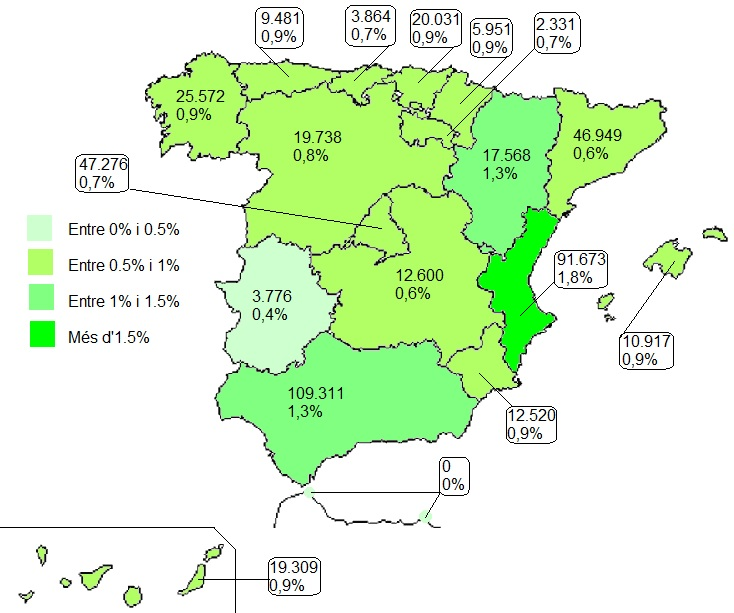
\includegraphics[scale = 0.6]{images/distribucio territorial en base a percentatge.jpg}
    \caption{Coloració geogràfica dels casos enregistrats de persones amb demència l'any 2019 (en la BDCAP) segons el tant per cent respecte a la població de cada comunitat autònoma.}
    \label{fig:colorpercent}
\end{figure}
\begin{figure}[H]
    \centering
    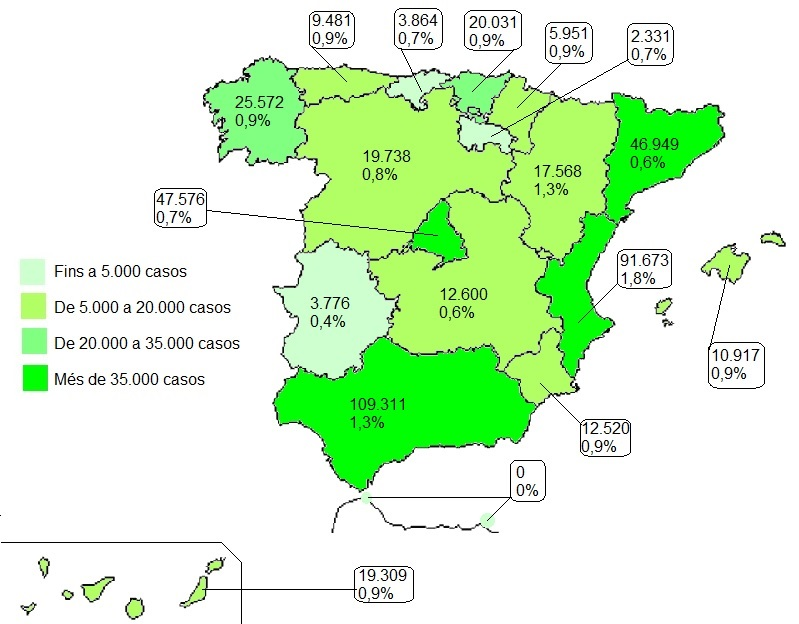
\includegraphics[scale = 0.6]{images/distribucio territorial en base a casos.jpg}
    \caption{Coloració geogràfica dels casos enregistrats de persones amb demència l'any 2019 (en la BDCAP) segons el nombre de casos.}
    \label{fig:colorcasos}
\end{figure}
Si es fa una comparació entre els dos mapes, s'observa que la coloració de moltes de les comunitats autònomes canvia, perquè no totes les comunitats autònomes tenen el mateix nombre d'habitants.\\
Abans de finalitzar aquesta secció, és necessari donar les dades de la taula \ref{tab:taula1} segregades per sexe i comunitat autònoma per tenir una idea encara més clara de com es distribueix la malaltia en el regne d'Espanya.
\begin{table}[h]
    \centering
    \begin{tabular}{ |c | c | c | c | c | c | } 
        \hline
        \hline Comunitat autònoma & \multicolumn{2}{|c|}{Home} & \multicolumn{2}{|c|}{Dona} & Total\\
        \hline
        Andalusia & 32.817 & 30\% & 76.494 & 70\% & 109.311\\
        \hline
        Aragó & 5.830 & 33,2\% & 11.739 & 66,8\% & 17.568\\
        \hline
        Astúries & 2.556 & 27\% & 6.924 & 73\% & 9.481\\
        \hline
        Illes Balears & 3.318 & 30,4\% & 7.958 & 69,6\% & 10.917\\
        \hline
        Illes Canàries & 6.169 & 31,9\% & 13.139 & 68\% & 19.309\\
        \hline
        Cantàbria & 1.024 & 26,5\% & 2.840 & 73,5\% & 3.864\\
         \hline
        Castella i Lleó & 5.611 & 28,4\% & 14.128 & 71,6\% & 19.738\\
         \hline
        Castella la Manxa & 4.091 & 32,5\% & 8.509 & 67,5\% & 12.600\\
         \hline
        Catalunya & 13.952 & 29,7\% & 32.998 & 70,3\% & 46.949\\
         \hline
        Comunitat Valenciana & 29.395 & 32,1\% & 62.278 & 67,9\% & 91.673\\
         \hline
        Extremadura & 1.231 & 32,6\% & 2.545 & 67,4\% & 3.776\\
         \hline
        Galícia & 7.161 & 28\% & 18.411 & 72\% & 25.572\\
         \hline
        Comunitat de Madrid & 15.586 & 30,9\% & 32.689 & 69,1\% & 47.276\\
         \hline
        Regió de Múrcia & 4.265 & 34,1\% & 8.256 & 65,9\% & 12.520\\
         \hline
        Comunitat foral de Navarra & 1.755 & 29,5\% & 4.196 & 70,5\% & 5.951\\
         \hline
        Euskal Herria & 5.719 & 28,6\% & 14.312 & 71,4\% & 20.031\\
         \hline
        La Rioja & 767 & 32,9\% & 1.564 & 67,1\% & 2.331\\
         \hline
        Ceuta & NA & NA & NA & NA & NA\\
        \hline
        Melilla & NA & NA & NA & NA & NA\\
        \hline
        Total & 140.248 & 30,6\% & 318.621 & 69,4\% & 458.869\\
        \hline
    \end{tabular}
    \caption{Distribució territorial i per sexe dels casos enregistrats de persones amb demència l'any 2019 en la BDCAP}
    \label{tab:taula2}
\end{table}
\newpage
Un cop conegudes les dades del cens de persones amb demència, es pot saber fàcilment, quin és el rang de persones amb Alzheimer per cada comunitat autònoma i sexe. El nombre de casos d'Alzheimer estarà comprès entre el 60\% i el 80\% dels casos de demència que figuren a la taula \ref{tab:taula2}. Per tant, a Espanya, dels 140.248 casos de demència en homes, entre 84.149 i 112.199 seran causats per l'Alzheimer. En el cas de les dones, hi haurà entre  191.173 i 254.897 casos d'Alzheimer. En el cas del total hi haurà entre 275.322 i 367.096 casos demència causats per Alzheimer.
\section*{Principals associacions de lluita contra l'Alzheimer}
\addcontentsline{toc}{section}{Principals associacions de lluita contra l'Alzheimer}
A escala de tota Espanya hi ha moltes associacions sense ànim de lucre que es dediquen a lluitar per trobar un remei a aquesta malaltia que cada dia afecta a més gent. Com és molt difícil poder anomenar totes les associacions del país, només es llistaran les més importants.
\begin{itemize}
    \item \href{https://fpmaragall.org/ca/}{\underline{Fundació Pasqual Maragall}}
    \item \href{https://www.ceafa.es/es}{\underline{Confederació espanyola de familiars malalts d'Alzheimer i altres demències}}
    \item \href{http://www.alzfae.org/}{\underline{Fundació Alzheimer Espanya}}
    \item \href{https://www.afav.org/}{\underline{Associació familiars Alzheimer València}}
    \item \href{https://www.fevafa.org/quienes-somos/}{\underline{Federació valenciana d'associacions de familiars i amics de persones amb Alzheimer}}
    \item \href{https://www.fafac.cat/}{\underline{Federació catalana Alzheimer}}
    \item \href{http://www.lleidaparticipa.cat/index_web.php?idwc=czoxNToiYWx6aGVpbWVybGxlaWRhIjs=}{\underline{Associació de familiars de malalts d'Alzheimer i altres demències de Lleida}}
    \item \href{https://afamur.es/que-es-afamur/}{\underline{\textit{Asociación de familiares enfermos de Alzheimer de la Región de Múrcia}}}
    \item \href{https://fafal.org/}{\underline{\textit{Federación de asociaciones de familiares enfermos de Alzheimer de la CM}}}
    \item \href{https://www.afacayle.es/}{\underline{\textit{Federación regional de asociaciones de familiares de enfermos de Alzheimer de CyL}}}
    \item \href{https://www.alzheimersevilla.com/}{\underline{\textit{Asociación de familiares de enfermos de Alzherimer Santa Elena}}}
    \item \href{https://afaga.com/es/asociacion/historia/}{\underline{\textit{Asociación de familiares de enfermos de Alzherimer y otras demencias de Galicia}}}
    \item \href{https://www.asociacionalzheimer.com/}{\underline{\textit{Asociación Alzheimer Asturias}}}
\end{itemize}
\section*{Experiència personal amb la malaltia}
\addcontentsline{toc}{section}{Experiència personal amb la malaltia}
La meva àvia paterna va morir l'any 2008, des d'aleshores, el meu avi no va tornar a ser el mateix... Va començar a oblidar algunes coses que ell feia de manera diària, on posava segons quines coses, alguna data important, etc. Mentre això no anava a més, a la família no ens preocupava el més mínim aquesta simptomatologia atès que la mort de la meva àvia, la seva dona, va ser el desencadenant perquè el meu avi fos diagnosticat amb depressió. Malgrat això, quan els símptomes es varen anar agreujant, la família ens vam adonar que alguna cosa estranya passava i després d'una sèrie de proves clíniques, el meu avi va ser diagnosticat amb Alzheimer.\\
Va ser un moment molt dur per la família. Veure que una algú que, durant tota la vida, havia estat molt activa, de fer bromes, de fer plans familiars, cuinar, etc. ara ja només podia anar en caiguda lliure cap a la desconnexió mental total. A mesura que passava el temps, l'actitud del meu avi també va canviar. Al principi, no se'n recordava de dutxar-se, després va començar a oblidar on posava les coses (fet que el va portar a acusar a la família de robar-lo) i va desenvolupar una obsessió molt forta pels diners. Quan la situació es va fer insostenible, el meu pare i les seves dues germanes, amb el diagnòstic d'Alzheimer a la mà varen anar al jutjat a demanar la incapacitació total del meu padrí. Després de revisar l'informe mèdic i fer-li algunes preguntes, la jutgessa va decretar que des d'aquell precís moment, la signatura del meu avi deixava de tenir qualsevol validesa legal.\\
Mentre la família esperàvem a la concessió d'una plaça pública en una residència, el meu pare i les seves germanes decidiren internar al meu avi en una residència privada. En aquesta residència, feia tota mena d'activitats per potenciar la memòria, però maluradament cap va tenir el més mínim efecte. Al cap de poc temps d'estar en la residència, les visites cada cop es feien més pesades, tristes i difícils, ja que el meu avi va començar a confondre a la família amb altres persones. Per exemple, jo, en comptes del seu nét, era el seu germà. El meu pare, en comptes del seu fill, era el seu pare i les meves tietes les seves cosines. Amb altres membres de la família, com poden ser la meva mare i els meus cosins, la situació era idèntica.\\
Passats uns anys, la plaça pública va arribar. El meu avi va ser traslladat a una residència d'Alcarràs. La família teníem una petita esperança que el canvi de residència li dones, al meu avi, una mica d'aire i tornés per uns dies al seu ser. Lluny d'aquest desig, el meu avi continuava en caiguda lliure cap a la mort en vida. Poc abans de morir, no era capaç ni d'aixecar-se de la cadira i fer un sol pas sense anar agafat del braç. Els dies previs a la seva mort, ni tan sols es llevava del llit. Els metges decidiren administrar-li morfina i a les sis de la tarda del 17 de novembre de l'any 2015, l'àngel de la mort aparegué a l'habitació i s'endugué la seva ànima.
\chapter*{Marc teòric computacional}
\addcontentsline{toc}{chapter}{Marc teòric computacional}
\section*{Qué entenem per intel·ligència artificial?}
\addcontentsline{toc}{section}{Que entenem per intel·ligència artificial?}
La història de la intel·ligència artificial neix l'any 1950, quan Alan Turing publica el llibre "\textit{Computing machinery and intelligence}". En aquest llibre es planteja, per primer cop, que les màquines poden pensar. Des d'aleshores, la IA ha acumulat successos i nefastos fracassos.\\
\begin{figure}[H]
    \centering
    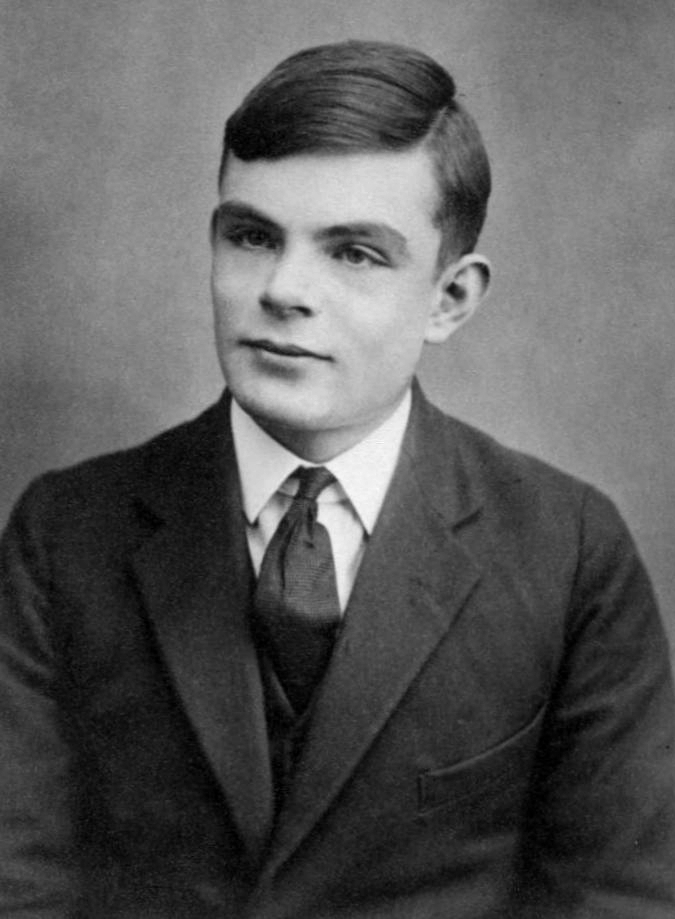
\includegraphics[scale = 0.2]{images/Alan_Turing_Aged_16.jpg}
    \caption{Retrat d'Alan Turing}
    \label{fig:turing}
\end{figure}
S'entén per intel·ligència artificial la capacitat que té una màquina d'adquirir aptituds relacionades amb els éssers humans. Aquestes aptituds inclouen el raonament i l'aprenentatge, entre d'altres. Dit d'altra manera, la IA és un conjunt d'algorismes que pretén fer que les màquines imitin el comportament humà.\\
Segons els informàtics experts, \textit{Stuart Russell} (Figrua \ref{fig:russell}) i \textit{Peter Norvig} (Figura \ref{fig:norvig}), existeixen quatre tipus diferents d'intel·ligències artificials.
\begin{figure}[h!]
    \centering
    \begin{subfigure}[b]{0.48\linewidth}
        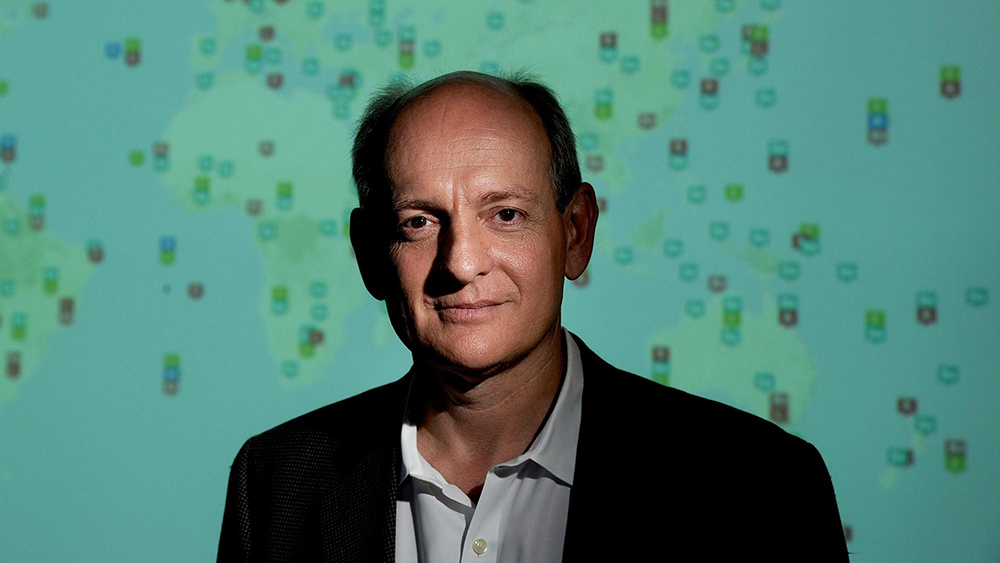
\includegraphics[width=\linewidth]{images/russell-aqua.jpg}
        \caption{Retrat de Stuart Russell}
        \label{fig:russell}
    \end{subfigure}
    \begin{subfigure}[b]{0.45\linewidth}
        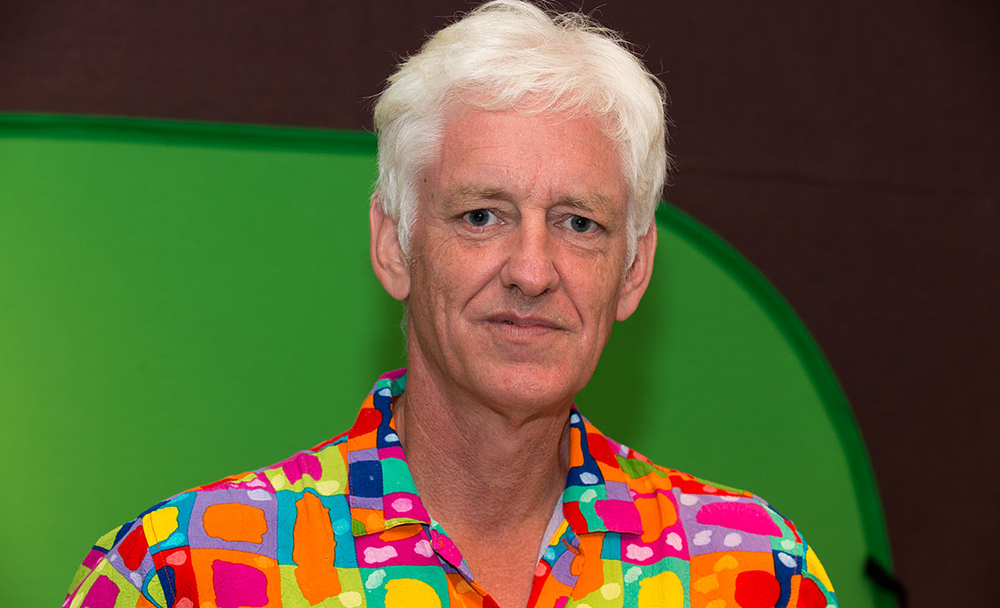
\includegraphics[width=\linewidth]{images/peter_norvig_speaking_at_university_of_california_berkeley_2013.jpg}
        \caption{Retrat de Peter Norvig}
        \label{fig:norvig}
    \end{subfigure}
    \caption{Retrats dels científics Stuart Russell (esquerra) i Peter Norvig (dreta)}
    \label{fig:StuartNorvig}
\end{figure}
El primer tipus són aquells sistemes que pensen com els humans, és a dir, són aquells sistemes que automatitzen tasques com prendre decisions, resoldre problemes, etc. Un exemple d'aquest tipus de IA són les xarxes neuronals.\\
A continuació, es troben aquelles IA capaces de recrear el comportament humà. Aquest tipus de sistemes són computadores que duen a terme diferents tasques de la mateixa manera que ho faria un humà. El cas més evident són els robots.\\
En tercer lloc, es troben els sistemes de pensament racional, que són aquells que intenten copiar la lògica racional del pensament de les persones. Dit en altres paraules, es tracta d'aconseguir màquines que puguin disposar de la capacitat de percebre un estímul, jutjar-lo i actuar conseqüentment a aquell estímul. En aquest grup, s'engloben els sistemes experts. Aquests sistemes poden ser sistemes RBR (\textit{Rule Based Reasoning}), sistemes CBR (\textit{Case Based Reasoning}) o sistemes basats en xarxes bayesianes.\\
La quarta, i última forma en què es presenta la IA, són els sistemes que actuen de manera racional. Aquests sistemes són aquells que intenten copiar la forma de comportament humana. És el cas dels sistemes intel·ligents.
\section*{Avantatges i desavantatges de la IA}
\addcontentsline{toc}{section}{Avantatges i desavantatges de la IA}
Tenint en compte les defenses de la IA per part de \textit{Andy Chan} (Figure \ref{fig:chan}), \textit{Product Manager} de Infinia ML, i \textit{Kai-Fu Lee} (Figura \ref{fig:lee}), fundador del fons de capital de risc Sinovation Ventures, els avantatges de la intel·ligència artificial serien:
\begin{itemize}
    \item Automatització de processos.
    \item Potenciació de les tasques creatives.
    \item Precisió.
    \item Reducció de l'error humà.
    \item Reducció del temps emprat en l'anàlisi de dades.
    \item Manteniment predictiu.
    \item Millora en la presa de decisions a escala productiva i de negoci.
    \item Control i optimització de processos productius i línies de producció.
    \item Augment de la productivitat i de la qualitat de la producció.
\end{itemize}
Un cop vistos els avantatges, toca veure la part dolenta de la intel·ligència artificial. Com tot, no hi ha res perfecte i que no comporti riscos i conseqüències.
\begin{itemize}
    \item Disponibilitat de dades.
    \item Insuficiència de personal amb la qualificació adequada.
    \item Cost i temps d'implementació dels projectes.
\end{itemize}
\begin{figure}[h!]
    \centering
    \begin{subfigure}[b]{0.45\linewidth}
        
\includegraphics[width=\linewidth]{images/1565701087600.jpg}
        \caption{Retrat d'Andy Chan}
        \label{fig:chan}
    \end{subfigure}
    \begin{subfigure}[b]{0.47\linewidth}
        
\includegraphics[width=\linewidth]{images/Capture_medium.jpg}
        \caption{Retrat de Kai-Fu Lee}
        \label{fig:lee}
    \end{subfigure}
    \caption{Retrats d'Andy Chan (esquerra) i Kai-Fu Lee (dreta)}
    \label{fig:AndyKai}
\end{figure}
\section*{Qué és el \textit{Machine Learning}?}
\addcontentsline{toc}{section}{Que és el \textit{Machine Learning}?}
Es defineix com \textit{Machine Learning} la disciplina que atorga, als ordinadors, la capacitat d'aprendre de manera autònoma patrons en dades massives i elaborar prediccions.\\
En paraules de \textit{Jeff Hawkins} (Figura \ref{fig:hawkins}):
\begin{center}
    \begin{minipage}{0.9\linewidth}
        \vspace{5pt}
        {\small
            El \textit{Machine Learning} és la capacitat de predir el futur, per exemple, el pes d'un got que volem aixecar o la reacció de les persones als nostres actes, d'acord amb els patrons emmagatzemats en la memòria.
        }
        \vspace{5pt}
    \end{minipage}
\end{center}
\begin{figure}[H]
    \centering
    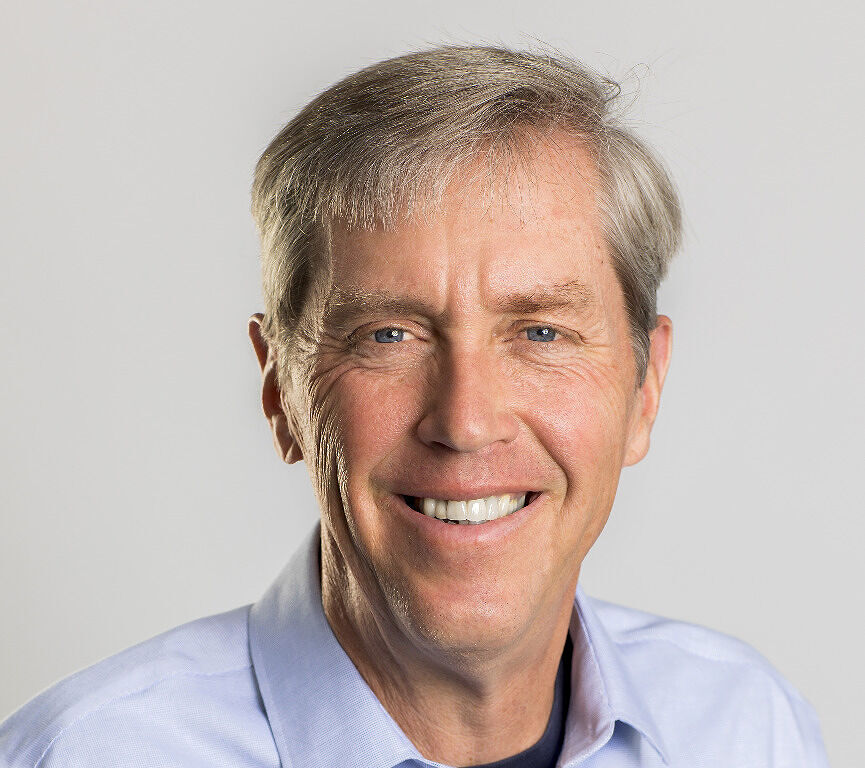
\includegraphics[scale = 0.3]{images/b2a43a485uokuohjp5l7peo9f0.jpg}
    \caption{Retrat de \textit{Jeff Hawkins}}
    \label{fig:hawkins}
\end{figure}
\subsection*{Tipus de \textit{Machine Learning}}
\addcontentsline{toc}{subsection}{Tipus de \textit{Machine Learning}}
Ara com ara, existeixen quatre tipus diferents d'aprenentatge automàtic.\\
El primer tipus és, l'aprenentatge supervisat. Aquest tipus d'aprenentatge, és aquell en el qual especifiquem a l'algorisme quina cosa ha d'aprendre i, un cop après, el model intel·ligent u seguirà al peu de la lletra. Dit més formalment, un model intel·ligent que utilitza aprenentatge supervisat és, aquell que ha estat entrenat amb una base de dades perfectament etiquetada i que realitza prediccions molt específiques basant-se en les etiquetes. Dos exemples d'ús d'aquest tipus d'aprenentatge podrien ser els classificadors d'imatges i els classificadors de so.\\
El segon tipus d'aprenentatge és el no supervisat. L'objectiu d'aquest tipus d'aprenentatge és, que el programari aprengui per si mateix sense ajuda dels científics de dades a partir d'un conjunt de dades etiquetades. És a dir, aquesta tècnica de \textit{Machine Learning}, es basa en el fet que són els mateixos models els que troben patrons existents en les dades a analitzar.\\
Dins de l'aprenentatge no supervisat, es poden diferenciar dos subtipus. El primer és el \textit{Clustering} que permet identificar les agrupacions naturals resultants de l'anàlisi de totes les dades i, el segon, és l'\textit{Association} que permet descobrir les relacions entre les variables en un gran volum de dades.\\
El penúltim tipus de \textit{Machine Learning} és, l'aprenentatge semisupervisat. Aquest tipus d'aprenentatge és, una mescla dels dos anteriors, ja que utilitza un grup mínim d'etiquetes. La gran majoria de les dades són dades que no estan etiquetades, perquè tot i que les dades sense etiquetar augmenten els costos, són útils per aconseguir els objectius.\\
Tot i que sí que hi ha una supervisió per part del programador, no és una tasca que es realitzarà al llarg del procés d'aprenentatge (Algunes dades sí que s'etiqueten a mà, però la resta les etiquetarà l'algorisme).\\
Aquest tipus d'aprenentatge també es pot usar per a la classificació d'imatges. En aquest cas, es dona un subconjunt d'imatges etiquetades i un subconjunt sense etiquetes. El model s'ajudarà de les imatges etiquetades per classificar les no etiquetades.\\
Un segon exemple d'utilització d'aquesta tècnica, és la detecció de frau fiscal en transaccions financeres. El procediment és igual que abans; es tenen una sèrie de transaccions etiquetades com a frau (o com a no frau) i una sèrie de transaccions sense etiquetar. El model usarà les dades etiquetades per aprendre a detectar transaccions fraudulentes i també utilitzarà les dades no etiquetades per millorar la precisió a l'hora de detectar si una transacció és fraudulenta o no.\\
L'últim tipus d'aprenentatge automàtic és l'aprenentatge per reforç. La principal característica de l'aprenentatge per reforç és que és capaç de funcionar sense grans quantitats de dades. En aquesta tècnica, la IA guia el seu propi aprenentatge (explora un entorn desconegut) mitjançant un sistema de recompenses i càstigs. És a dir, és un sistema que guia el seu aprenentatge segons la tècnica de "prova i error".\\
El sistema de recompenses i càstigs comporta, no solament que, el model aprengui de manera immediata sinó que busqui maximitzar la recompensa.
Un exemple molt clar d'aquest tipus de sistemes són els robots. El robot rebrà una recompensa o un càstig segons realitzi bé, o no, una determinada acció. Un exemple de recompensa, per exemple, podria ser augmentar un punt en un sistema de puntuació. Per contra, el càstig, disminuiria un punt.\\
Aquest tipus d'aprenentatge també es pot extrapolar a la vida real. L'entrenament de gossos en seria un cas. L'entrenador ensenya una ordre a l'animal i aquest rebrà una galeta com a premi, si ho fa bé, o se li posarà el morrió si ho fa malament.
\section*{Qué és una xarxa neuronal?}
\addcontentsline{toc}{section}{Qué és una xarxa neuronal?}
Les xarxes neuronals són models matemàtics que imiten el processament d'una certa informació tal com ho faria el cervell humà. Atès que el seu objectiu és emular el comportament d'un cervell, una xarxa està composta per neurones i capes (igual que un cervell humà). Les neurones es transmeten senyals entre elles. Aquests senyals es transmeten des de l'entrada fins a la generació d'una sortida.\\
Segons la topologia de la xarxa, hi ha cinc possibles classificacions de xarxes neuronals artificials (ANN en són les sigles en anglès, que es corresponen a \textit{Artifficial Neural Network}).\\
El primer tipus són les xarxes monocapa. Són les xarxes més senzilles, ja que només consten d'una capa d'entrada i una de sortida.\\
En segon lloc, hi ha les xarxes multicapa. Aquest tipus de xarxes són, una generalització de l'anterior. Aquestes contenen una sèrie de capes intermèdies entre la capa d'entrada i la de sortida. Aquestes capes intermèdies s'anomenen ocultes.\\
Depenent del nombre de connexions, la xarxa serà, o bé, completament connectada, o bé, parcialment connectada. Les xarxes completament connectades, són aquelles en les que cada neurona de cada capa està connectada a cada neurona de la següent capa (capes denses). En canvi, les xarxes parcialment connectades, són aquelles en les que no totes les neurones d'una capa estan connectades amb totes les neurones de la següent capa.\\
Un tercer tipus de xarxes neuronals, són les xarxes convolucionals (tècnica utilitzada per al desenvolupament dels diferents experiments). Aquest tipus de xarxes, són xarxes en les quals cada neurona no està connectada a totes les neurones de la següent capa. A més, les xarxes convolucionals (CNN en anglès), compten amb diverses capes ocultes especialitzades i amb una jerarquia. Això significa que les primeres capes detecten elements genèrics com poden ser línies o corbes i, tal com s'avança en les capes convolucionals, cada cop més especialitzades, s'arriba a les capes més profundes que reconeixen formes complexes com podria ser una cara.\\
El quart tipus de xarxes, són les xarxes recurrents. Aquestes xarxes no s'estructuren amb capes. Aquest tipus d'\textit{ANN} permeten connexions aleatòries que poden arribar a crear cicles, fet que permet que la xarxa tingui memòria.\\
Les dades es transformen i circulen per la xarxa no només en l'instant "t", sinó que també poden circular en l'instant "t + x", essent x un nombre natural.\\
L'últim tipus de xarxes neuronals són les xarxes de base radial. Aquest tipus de xarxes es caracteritza per tenir una capa d'entrada, una única capa oculta i una capa de sortida. Les neurones d'aquest tipus de xarxes usen les denominades funcions d'activació de base radial i la sortida de la xarxa es calcula com una combinació lineal de les sortides de cada neurona.
\subsection*{Qué compon una xarxa neuronal?}
\addcontentsline{toc}{subsection}{Qué compon una xarxa neuronal?}
La unitat de processament bàsica d'una xarxa neuronal són les neurones, que s'ordenen en capes. Per tant, es podria veure una capa com una caixa plena de pilotes on cada pilota representa una neurona.\\
Normalment, en una xarxa neuronal artificial (ANN en anglès), es poden diferenciar tres parts diferents: la capa d'entrada, les capes ocultes (si n'hi ha) i la capa de sortida.\\
La capa d'entrada, com el seu nom indica, representa tots els camps que s'entren a la xarxa per ser processats. Aquesta capa estarà formada per una o més neurones.\\
En segon lloc, estan les capes ocultes. Cal remarcar que aquest tipus de capes, poden no existir en la xarxa, és a dir, és possible que la xarxa estigui composta, exclusivament, per una capa d'entrada i una capa de sortida (xarxa monocapa). També existeix la possibilitat que, en comptes d'haver-hi diverses capes ocultes, solament n'hi hagi una. Cada capa oculta estarà formada per una o més neurones.\\
Finalment, la capa de sortida, és una capa que tindrà tantes neurones com resultats puguin tenir les dades processades. És a dir, en el cas d'aquest treball, la xarxa s'encarrega de classificar imatges entre quatre nivells diferents d'Alzheimer, per tant, la xarxa tindrà una totalitat de 4 neurones a la capa de sortida.\\
Com s'ha esmentat, les neurones estan organitzades per capes. Cada neurona es relaciona mitjançant "pesos" amb algunes (o totes) les neurones de la següent capa, així, les dades es presenten en la primera capa (la d'entrada) i els valors es propaguen des de la neurona en la qual es troben en aquell moment fins a totes aquelles neurones de la capa següent amb les quals hi hagi una relació. Finalment, els resultats arribaran a la capa de sortida, on es podran observar els resultats.
\section*{Xarxes neuronals convolucionals (CNN)}
\addcontentsline{toc}{section}{Xarxes neuronals convolucionals (CNN)}
Les xarxes neuronals convolucionals són, un algorisme de \textit{deep learning} que estan dissenyades per l'anàlisi d'atributs visuals de grans quantitats de dades. Tot i que, normalment, s'utilitzen en aspectes relacionats amb les imatges, les CNN tenen més aplicacions dins del món de la intel·ligència artificial. Aquests altres menesters inclouen el processament del llenguatge natural, per exemple.\\
Com tota xarxa utilitzada per a classificar, aquestes xarxes, en primer lloc, han de realitzar una fase d'extracció de característiques. D'aquesta fase se n'encarreguen les neurones convolucionals. Seguidament, es realitza una reducció per mostreig (\textit{pooling} en aquest cas) i finalment, es troben una sèrie de neurones més senzilles que permeten realitzar la classificació de les característiques que s'han extret prèviament.\\
En aquesta fase d'extracció de característiques es pot trobar una similitud molt elevada amb el procés d'estimulació cel·lular del còrtex visual del cervell humà.\\
Per dur a terme amb èxit aquesta fase, es van alternant capes de convolució i capes de reducció (\textit{pooling}). A mesura que les dades avancen cap a la sortida, cada cop es van fent més i més petites. D'aquesta manera les primeres capes són menys sensibles a canvis mentre que les capes finals són extremadament sensibles a qualsevol canvi i a qualsevol pertorbació en les dades d'entrada.
\section*{Entrenament de xarxes neuronals}
\addcontentsline{toc}{section}{Entrenament de xarxes neuronals}
Per entrenar una xarxa neuronal, cal exposar una gran quantitat d'entrades amb les seves respectives sortides. Durant l'entrenament, la xarxa anirà ajustant els pesos de les connexions entre neurones per tal de millorar el rendiment i poder prediccions en el futur. Per ajustar els pesos, la xarxa realitza complexos càlculs matemàtics que generen una sortida a partir d'una entrada per a posteriorment realitzar una comparació del càlcul obtingut amb la sortida real. Amb aquesta comparació de resultats s'obté un error que és l'utilitzat per ajustar els pesos de les connexions de la xarxa.\\
Aquest procés es repeteix un elevat nombre de vegades però no sempre amb la mateixa entrada i la mateixa sortida, sinó que les parelles \textit{input - output}, canvien. D'aquesta manera, al llarg del temps, la xarxa podrà ser capaç de realitzar, de manera precisa, prediccions amb dades d'entrada que no ha vist mai, és a dir, amb dades que no s'han utilitzat en el moment de l'entrenament.
\begin{figure}[H]
    \centering
    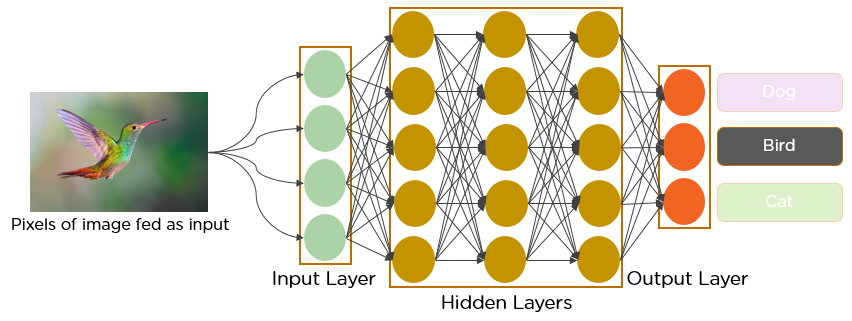
\includegraphics[scale = 0.5]{images/CNN.png}
    \caption{Exemple d'esquema d'una CNN}
    \label{fig:cnn}
\end{figure}
\chapter*{La IA en la lluita contra l'Alzheimer}
\addcontentsline{toc}{chapter}{La IA en la lluita contra l'Alzheimer}
En aquesta secció es presentaran una sèrie d'articles periodístics que mostres que, no solament és possible que la IA ajudi en la batalla contra l'Alzheimer, sinó que ho fa de manera molt efectiva.\\
La primera notícia es publica a \href{https://neurohouse.es/espacio-reimagine/la-inteligencia-artificial-una-nueva-aliada-contra-el-alzheimer}{\underline{\textit{Neuro House}}} el 22-10-2020 i es titula "\textit{La inteligencia artificial, una nueva aliada contra el Alzheimer}".
\begin{center}
    \begin{minipage}{0.9\linewidth}
        \vspace{5pt}
        {\small
            Gràcies als progressos tan grans que està havent-hi en el camp de la IA, és possible detectar casos d'Alzheimer fins amb quinze anys d'antelació, mitjançant l'estudi genètic i el monitoratge dels pacients. A més, està previst que de manera futura, la IA pugui servir per a la detecció d'altres afectacions mentals de caràcter mortal com podria ser, per exemple, la depressió.\\
            Investigadors de la Universitat de Califòrnia, han desenvolupat una IA que és capaç de detectar la disminució del consum de glucosa, un dels primers símptomes de la malaltia d'Alzheimer.
        }
        \vspace{5pt}
    \end{minipage}
\end{center}
\newpage
El segon article va ser publicat al diari \href{https://www.lavanguardia.com/vida/20220427/8225520/inteligencia-artificial-ver-deterioro-cognitivo-acabara-alzheimer.html}{\underline{La Vanguardia}} el 27-04-2022 i porta per títol "\textit{Inteligencia artificial para ver si deterioro cognitivo acabará en Alzheimer}".
\begin{center}
    \begin{minipage}{0.9\linewidth}
        \vspace{5pt}
        {\small
            Alguns científics de la UOC han desenvolupat una IA que permet diagnosticar si el deteriorament cognitiu lleu progressarà fins a arribar a convertir-se en Alzheimer.\\
            Aquesta IA utilitza mètodes molt específics per reconèixer imatges de MRI i supera l'eficàcia de tots els mètodes emprats fins al moment, segons la investigadora Mona Ashtari-Majlan.\\
            Per desenvolupar aquesta intel·ligència, els investigadors, han fet servir el mètode de les xarxes neuronals convolucionals de múltiples fluxes, que és una tècnica d'intel·ligència artificial i de \textit{deep learning} molt útil per la classificació d'imatges.\\
            En primer lloc, l'equip d'investigació, va comprar imatges de MRI de persones amb Alzheimer i de persones sanes, cosa que va permetre buscar diferents punts de referència. Després d'entrenar el model, van realitzar un ajustament d'aquest amb imatges de persones amb una diagnosi de deteriorament cognitiu lleu.\\
            Amb un total de quasi 700 imatges de bases de dades públiques, el model és capaç de diferenciar si el deteriorament cognitiu lleu arribarà a ser Alzheimer, o no, amb un 85\% de precisió.
        }
        \vspace{5pt}
    \end{minipage}
\end{center}
Per tal d'obtenir una informació una mica més tècnica sobre aquesta proposta, s'ha consultat la publicació original dels autors. En ella s'observa com la proposta de recerca que fan es basa en 2 passos. El primer dels passos ha consistit a desenvolupar un enfocament basat en les dades. Aquest nou enfocament utilitza una tècnica del camp de l'estadística anomenada \textit{\href{https://www.statisticshowto.com/hotellings-t-squared/}{\underline{Hotelling's T-squared distribution}}} que consisteix a comparar els valors de les mitjanes dels grups de classificació per poder determinar si els diferents grups tenen, en termes de multivariabilitat, diferències estadístiques significatives o, si senzillament, són variacions aleatòries. Gràcies a l'aplicació d'aquesta tècnica, l'equip investigador, aconsegueix crear un mapa en forma de cervell tot identificant diferents aspectes anatòmics. Cadascun d'aquests punts s'associa a una coordenada en 3 dimensions de la qual s'extreu un fragment d'imatge de 19x19x19 píxels.\\
Per obtenir la mitjana d'un dels anomenats punts anatòmics clau, el que es fa és sumar totes les mesures d'aquell punt i dividir la suma entre el nombre de mostres. Aquest càlcul es realitza per cadascun dels punts clau i per cada possible classe de classificació. Aleshores, un cop obtingudes totes les mitjanes de totes les classes, es pot dur a terme la comparació i concloure si les diferències són aleatòries o no.\\
El segon pas d'aquesta recerca ha estat implementar una xarxa neuronal convolucional multiflux, on cada flux s'alimenta d'un dels fragments d'imatge de 19x19x19.\\
Els investigadors han avaluat el rendiment d'aquest mètode en tres passos experimentals (entrenar el model convolucional de flux múltiple amb imatges de MRI, transferir els pesos del model entrenat a una arquitectura idèntica tot ajustant-la amb dades relacionades amb pacients sMCI i pMCI i afegir biomarcadors) i després de realitzar uns quants experiments, els resultats d'aquests demostra que el mètode supera qualsevol altre enfocament existent per la diagnosi de la malaltia.\\
La tercera, i última, notícia es va publicar al diari \href{https://www.larazon.es/sociedad/20220620/ajwe2fywxzgnta7zt4godk4bae.html}{\underline{\textit{La Razón}}} el 7-11-2022 i es titula "\textit{Una nueva prueba para el diagnóstico precoz del Alzheimer logra una efectividad del 98\%}".
\begin{center}
    \begin{minipage}{0.9\linewidth}
        \vspace{5pt}
        {\small
            Un grup d'investigadors de l'\textit{Imperial College of London} han combinat un sistema d'aprenentatge automàtic amb una imatge d'un MRI cerebral per crear un sistema intel·ligent que és capaç de detectar l'Alzheimer en el 98\% dels casos. En el Regne Unit s'ha dut a terme una prova amb 400 individus i l'algorisme ha diagnosticat correctament la malaltia en el 98\% dels casos i, inclús, ha estat capaç de diferenciar l'etapa primerenca de l'etapa avançada de l'Alzheimer en un 79\% dels pacients.\\
            Aquesta tecnologia, molt més senzilla d'usar que les proves actuals, és capaç d'identificar la malaltia d'Alzheimer en les etapes primerenques, quan encara la patologia és molt difícil de diagnosticar. Aquesta tecnologia, inclús, es fixa en zones de l'estructura cerebral que mai han estat associades amb la malaltia.\\
            \begin{center}
                \begin{minipage}{0.9\linewidth}
                    \vspace{5pt}
                    {\small \textit{Waiting for a diagnosis can be a horrible experience for patients and their families. If we could reduce the amount of time they have to wait, make the diagnosis a simpler process and reduce some of the uncertainity, it would be helpful.}
                    }
                    \vspace{20pt}
                \end{minipage}
            \end{center}
            Aquestes van ser les paraules del professor de farmacologia del càncer en l'\textit{Imperial College of London} i investigador del projecte \textit{Eric Aboagye} en un comunicat de premsa.\\
            \begin{center}
                \begin{minipage}{0.9\linewidth}
                    \vspace{5pt}
                    {\small \textit{While neuroradiologists interpret the MRI to help to diagnose the AD, It's probable that are some characteristics that are not visible in the explorations, even for the specialists. Using an algorithm able to select subtle textures and structural characteristics on the brain that are affected because of the Alzheimer, actually could improve the information that we can obtain in the standard-imaging techniques.}
                    }
                    \vspace{20pt}
                \end{minipage}
            \end{center}
            Afirma el neuròleg \textit{Paresh Mahotra}, investigador del departament de ciències del cervell.
        }
        \vspace{5pt}
    \end{minipage}
\end{center}
De la mateixa manera que en l'última notícia, s'ha consultat la publicació oficial del grup d'investigació per tal de poder obtenir una informació més detallada de la proposta implementada.\\
En aquesta recerca, s'ha dissenyat un enfocament d'un operador de selecció i contracció mínima absoluta en dos passos (LASSO son les sigles en anglès). Les imatges seleccionades per l'entrenament del model són imatges per ressonància magnètica del tipus T1w que han estat segmentades en un total de 115 regions mitjançant la funció de reconeixement de \textit{FreeSurfer}. Després de la selecció i estandardització de les imatges s'ha creat un primer operador de contracció i selecció (LASSO1) que s'encarrega de classificar entre les persones amb patologia i sense patologia relacionada amb l'Alzheimer. Dins d'aquest, es crea un segon operador (LASSO2) que s'encarrega de diferenciar entre pacients amb un deteriorament cognitiu lleu causat per Alzheimer i pacients amb Alzheimer. Aquest model també ha estat integrat amb altres puntuacions cognitives com el \textit{Mini-Mental State Examination} (\href{https://www.farmaceuticoscomunitarios.org/anexos/vol11_n1/ANEXO2.pdf}{\underline{MMSE}} en anglès), que és una prova curta, d'uns 10 minuts de llargada, i estructurada de l'estat mental del pacient.\\
Com el model final, només ha de discriminar entre persones amb patologies relacionades amb la malaltia d'Alzheimer i persones amb patologies no relacionades amb la malaltia d'Alzheimer, es va introduir en un grup de patologies anomenat \textit{non-AD-related} els casos de persones sanes, persones amb Parkinson, demència frontotemporal, etc.
\chapter*{Implementació de la proposta de treball i anàlisi de resultats}
\addcontentsline{toc}{chapter}{Implementació de la proposta de treball i anàlisi de resultats}
\section*{Disseny dels experiments}
\addcontentsline{toc}{section}{Disseny dels experiments}
 En aquesta secció hi haurà continguts diversos aspectes com: aclariments del codi, les característiques de la màquina i de l'entorn de programació on s'han realitzat tant els entrenaments de la xarxa com les proves, les llibreries utilitzades, anàlisis gràfiques i numèriques i l'anàlisi de les prediccions de manera gràfica.
\subsection*{Característiques de la màquina i de l'entorn de programació}
\addcontentsline{toc}{subsection}{Característiques de la màquina i de l'entorn de programació}
\textbf{\underline{Característiques del PC:}}
\begin{itemize}
    \item Sistema operatiu: Windows 10 Pro 64-bit
    \item CPU: Intel Core i7-3770K (8 CPUs) ~3.5GHz
    \item RAM: 8GB
    \item Disc: Western Digital Blue WD10EZEX 1TB
\end{itemize}
\textbf{\underline{Característiques de l'entorn de programació:}}
L'entorn de programació utilitzat és una llibreta \textit{Google Colab} que usa el \textit{backend} de \textit{Google Compute Engine} i inclou els següents recursos:
\begin{itemize}
    \item RAM: 12.7 GB
    \item Disc: 107.7GB
\end{itemize}
\subsection*{Llibreries de Python utilitzades}
\addcontentsline{toc}{subsection}{Llibreries de Python utilitzades}
A continuació s'especificaran les llibreries utilitzades per implementar la proposta de treball, tot donant una petita explicació de l'especialització de cada llibreria.\\
La primera, i principal, llibreria utilitzada és \href{https://www.tensorflow.org/?hl=es-419}{\underline{TensorFlow}}. Aquesta és una llibreria de codi obert que permet detectar i desxifrar patrons i correlacions, d'un conjunt de dades, de manera que aquests es corresponguin a patrons i correlacions similars al raonament humà.\\
La segona llibreria és \href{https://keras.io}{\underline{Keras}}. Keras és un programari que té implementades moltes eines de treball necessàries per poder crear una xarxa neuronal com: capes, optimitzadors, funcions d'activació, etc. Keras està construïda sobre la plataforma TensorFlow, per tant, és possible executar un model de Keras sobre TensorFlow. I a més a més, és possible fer-ho de manera senzilla.\\
La següent llibreria és \href{https://docs.python.org/3/library/datetime.html}{\underline{\textit{datetime}}}. Aquesta llibreria proporciona una àmplia varietat de classes per representar i manipular dates i temps com, també, donar-los-hi el format desitjat i transforma'ls en una gran varietat de formats.\\
A continuació, la llibreria \href{https://docs.python.org/3/library/os.html}{\underline{os}}, que és una llibreria que permet als programes de Python realitzar interaccions amb el Sistema operatiu. Es podria comparar l'ús d'aquesta llibreria, d'alguna manera, amb treballar, directament, sobre la \textit{Command line}, però amb la diferència que la llibreria és una eina programàtica i, per tant, té la seva sintaxi i la \textit{Command line} té comandes específiques del sistema operatiu.\\
Seguidament, la llibreria \href{https://lime-ml.readthedocs.io/en/latest/}{\underline{\textit{Lime}}}. Aquesta llibreria permet donar una explicació a les prediccions dels models d'aprenentatge automàtic d'una manera molt senzilla i ràpida per a les persones. En el moment de fer una predicció i treure l'explicació per pantalla, es podrà veure la imatge que s'ha predit i unes zones acolorides. Aquestes zones acolorides són l'explicació.\\
La llibreria \href{https://numpy.org}{\underline{Numpy}}, és una llibreria de Python enfocada a oferir implementacions d'operacions bàsiques en la computació. Aquestes operacions inclouen: operacions matricials, creació i manipulació d'\textit{arrays} multidimensionals, operacions d'àlgebra lineal, operacions de lectura i escriptura de dades, transformades de Fourier, operacions estadístiques, etc. I tot d'una manera senzilla i ràpida.\\
Una altra llibreria utilitzada és la llibreria \href{https://docs.opencv.org/4.x/d6/d00/tutorial_py_root.html}{\underline{OpenCV}}. Aquesta llibreria s'especialitza en la visió artificial (entendre les característiques d'una imatge) en temps real. De fet, el nom de la llibreria, precisament, significa "Visió artificial oberta" (\textit{Open Computer Vision} en anglès). Algunes de les aplicacions d'aquesta llibreria són el reconeixement facial, la interacció persona-ordinador, la realitat augmentada, el reconeixement d'objectes, entre d'altres.\\
La penúltima llibreria és \href{https://matplotlib.org}{\underline{Matplotlib}}. Aquesta és una llibreria de codi obert especialitzada en la visualització i representació gràfica de dades en dues dimensions i tres dimensions de dades emmagatzemades en diferents estructures i objectes, com per exemple, llistes, \textit{arrays} NumPy i objectes de tipus \textit{Pandas}.\\
L'última llibreria utilitzada és \href{https://scikit-image.org}{\underline{scikit-image}} (encara que a la importació es vegi com \textit{skimage}). Aquesta llibreria conté una àmplia varietat d'eines per al tractament i maneig d'imatges. Algunes d'aquestes eines són el processament bàsic d'imatges, la seva segmentació, la detecció dels límits de les imatges i extracció de característiques, entre moltes altres operacions. 
\section*{Anàlisi de resultats}
\addcontentsline{toc}{section}{Anàlisi de resultats}
\subsection*{Representació gràfica de la \textit{accuracy} i de la pèrdua}
\addcontentsline{toc}{subsection}{Representació gràfica de la \textit{accuracy} i de la pèrdua}
En primer lloc, es presenten les gràfiques de la precisió del conjunt de dades d'entrenament. Abans, però, cal remarcar que les dades del model 1 no han estat representades atès que el primer model que es va generar és considerat com a nul perquè hi havia configurats malament els paràmetres corresponents a les mides de les imatges i, per tant, els resultats no serien verídics.
\begin{figure}[H]
    \centering
    \begin{tikzpicture}[scale = 1.6]
    \begin{axis} [
        xlabel = {$Epoch$},
        ylabel = {$Accuracy$},
        xmin = 0, xmax = 20,
        ymin = 0, ymax = 1.1,
        xtick = {1, 2, 3, 4, 5, 6, 7, 8, 9, 10, 11, 12, 13, 14, 15, 16, 17, 18, 19, 20},
        xticklabel style = {rotate = 75, anchor = east},
        ytick = {0, 0.1, 0.2, 0.3, 0.4, 0.5, 0.6, 0.7, 0.8, 0.9, 1, 1.1},
        legend pos = south east,
        ymajorgrids = true,
        xmajorgrids = true,
        grid style = dashed,
    ]
    \addplot [
        color = blue,
    ]
    coordinates {
        (1, 0.5099)(2, 0.5437)(3, 0.5740)(4, 0.5951)(5, 0.6337)(6, 0.6511)(7, 0.6694)(8, 0.7084)(9, 0.7427)(10, 0.7720)(11, 0.8002)(12, 0.8325)(13, 0.8650)(14, 0.8739)(15, 0.8865)
        };
        \addlegendentry{Model 2}
    
    \addplot[
        color = green,
    ]
    coordinates { 
        (1, 0.6290)(2, 0.7893)(3, 0.8759)(4, 0.9106)(5, 0.9558)(6, 0.9717)(7, 0.9731)(8, 0.9771)(9, 0.9877)(10, 0.9926)(11, 0.9928)(12, 0.9964)(13, 0.9914)(14, 0.9930)(15, 0.9932)
        };
        \addlegendentry{Model 3}

    \addplot[
        color = red,
    ]
    coordinates { 
        (1, 0.5233)(2, 0.6832)(3, 0.7903)(4, 0.8647)(5, 0.9240)(6, 0.9535)(7, 0.9659)(8, 0.9728)(9, 0.9752)(10, 0.9811)(11, 0.9880)(12, 0.9931)(13, 0.9951)(14, 0.9935)(15, 0.9937)       
        };
        \addlegendentry{Model 4}

    \addplot[
        color = olive,
    ]
    coordinates { 
        (1, 0.5544)(2, 0.6905)(3, 0.8040)(4, 0.8696)(5, 0.9117)(6, 0.9471)(7, 0.9756)(8, 0.9714)(9, 0.9716)(10, 0.9704)(11, 0.9769)(12, 0.9873)(13, 0.9911)       
        };
        \addlegendentry{Model 5}

    \addplot[
        color = magenta,
    ]
    coordinates { 
        (1, 0.6374)(2, 0.8332)(3, 0.9030)      
        };
        \addlegendentry{Model 6}

    \addplot[
        color = teal,
    ]
    coordinates { 
        (1, 0.6347)(2, 0.8170)(3, 0.8869)(4, 0.9138)      
        };
        \addlegendentry{Model 7}
    \end{axis}
    \end{tikzpicture}
    \caption{Representació gràfica de la precisió, en el conjunt d'entrenament, dels models al llarg de les èpoques}
    \label{fig:trainingAcc}
\end{figure}
Com s'observa la gràfica anterior en el conjunt de dades d'entrenament, la precisió augmenta de manera molt significativa a partir del model 3 (inclòs). Tot i que no es realitzarà un un canvi de \textit{dataset} per un amb més dades (més imatges) fins al model 6, la precisió augmenta de manera significativa quan es "juga" amb els hiperparàmetres. En aquest cas la \textit{batch size}. Ara bé, no tot és positiu, perquè, com es veurà posteriorment, en alguns dels models s'ha hagut de batallar amb \textit{overfitting}. Abans, però, es presenta la representació gràfica de la pèrdua de les dades d'entrenament.
\begin{figure}[H]
    \centering
    \begin{tikzpicture}[scale = 1.6]
    \begin{axis} [
        xlabel = {$Epoch$},
        ylabel = {$Loss$},
        xmin = 0, xmax = 20,
        ymin = 0, ymax = 2,
        xtick = {1, 2, 3, 4, 5, 6, 7, 8, 9, 10, 11, 12, 13, 14, 15, 16, 17, 18, 19, 20},
        xticklabel style = {rotate = 75, anchor = east},
        ytick = {0, 0.2, 0.4, 0.6, 0.8, 1, 1.2, 1.4, 1.6, 1.8, 2},
        legend pos = north east,
        ymajorgrids = true,
        xmajorgrids = true,
        grid style = dashed,
    ]
    \addplot [
        color = blue,
    ]
    coordinates {
        (1, 1.1591)(2, 1.0109)(3, 0.920)(4, 0.8734)(5, 0.7996)(6, 0.7675)(7, 0.7202)(8, 0.6708)(9, 0.5895)(10, 0.5269)(11, 0.4759)(12, 0.4092)(13, 0.3347)(14, 0.3147)(15, 0.2810)
        };
        \addlegendentry{Model 2}
    
    \addplot[
        color = green,
    ]
    coordinates { 
        (1, 1.0919)(2, 0.4924)(3, 0.3310)(4, 0.2370)(5, 0.1293)(6, 0.0889)(7, 0.0842)(8, 0.0661)(9, 0.0409)(10, 0.0268)(11, 0.0236)(12, 0.0172)(13, 0.0273)(14, 0.0287)(15, 0.0203)
        };
        \addlegendentry{Model 3}

    \addplot[
        color = red,
    ]
    coordinates { 
        (1, 1.7039)(2, 0.7287)(3, 0.5146)(4, 0.3451)(5, 0.2037)(6, 0.1331)(7, 0.0973)(8, 0.0826)(9, 0.0712)(10, 0.0572)(11, 0.0358)(12, 0.0243)(13, 0.0185)(14, 0.0211)(15, 0.0213)       
        };
        \addlegendentry{Model 4}

    \addplot[
        color = olive,
    ]
    coordinates { 
        (1, 1.2818)(2, 0.6979)(3, 0.4848)(4, 0.3233)(5, 0.2412)(6, 0.1458)(7, 0.0730)(8, 0.0788)(9, 0.0788)(10, 0.0929)(11, 0.0684)(12, 0.0433)(13, 0.0297)       
        };
        \addlegendentry{Model 5}

    \addplot[
        color = magenta,
    ]
    coordinates { 
        (1, 0.8833)(2, 0.4093)(3, 0.2470)      
        };
        \addlegendentry{Model 6}

    \addplot[
        color = teal,
    ]
    coordinates { 
        (1, 0.9037)(2, 0.4491)(3, 0.2868)(4, 0.2224)      
        };
        \addlegendentry{Model 7}
    \end{axis}
    \end{tikzpicture}
    \caption{Representació gràfica de la pèrdua, en el conjunt d'entrenament, dels models al llarg de les èpoques}
    \label{fig:trainingLoss}
\end{figure}
De la mateixa manera que el canvi en els valors dels hiperparàmetres i el canvi \textit{dataset} afecten la precisió del model, també afecta la pèrdua. Com s'observa, en el model 2 la pèrdua baixa de manera lenta, però en modificar la \textit{batch size}, els valors de la pèrdua descendeixen més ràpidament i també s'observa una millora en el moment del canvi del conjunt de dades.\\
Un cop vist com queden les dades, tant de precisió com de pèrdua, del conjunt d'entrenament, cal veure com queden representades les dades del conjunt de validació o \textit{testing}. En primer lloc, s'observen les dades de precisió del conjunt de \textit{testing}.
\begin{figure}[H]
    \centering
    \begin{tikzpicture}[scale = 1.6]
    \begin{axis} [
        xlabel = {$Epoch$},
        ylabel = {$Accuracy$},
        xmin = 0, xmax = 20,
        ymin = 0, ymax = 1.1,
        xtick = {1, 2, 3, 4, 5, 6, 7, 8, 9, 10, 11, 12, 13, 14, 15, 16, 17, 18, 19, 20},
        xticklabel style = {rotate = 75, anchor = east},
        ytick = {0, 0.1, 0.2, 0.3, 0.4, 0.5, 0.6, 0.7, 0.8, 0.9, 1, 1.1},
        legend style = {font = \tiny},
        legend pos = south east,
        ymajorgrids = true,
        xmajorgrids = true,
        grid style = dashed,
    ]
    \addplot [
        color = blue,
    ]
    coordinates {
        (1, 0.5)(2, 0.5425)(3, 0.5225)(4, 0.5942)(5, 0.5908)(6, 0.5933)(7, 0.59)(8, 0.5667)(9, 0.52)(10, 0.5092)(11, 0.6242)(12, 0.4642)(13, 0.6067)(14, 0.6417)(15, 0.6467)
        };
        \addlegendentry{Model 2}
    
    \addplot[
        color = green,
    ]
    coordinates { 
        (1, 0.5083)(2, 0.5733)(3, 0.5725)(4, 0.44)(5, 0.6792)(6, 0.6008)(7, 0.7050)(8, 0.4542)(9, 0.4483)(10, 0.5)(11, 0.71)(12, 0.6608)(13, 0.7317)(14, 0.7358)(15, 0.7483)
        };
        \addlegendentry{Model 3}

    \addplot[
        color = red,
    ]
    coordinates { 
        (1, 0.5425)(2, 0.4992)(3, 0.5025)(4, 0.5075)(5, 0.5008)(6, 0.5167)(7, 0.5858)(8, 0.6158)(9, 0.68)(10, 0.4117)(11, 0.6083)(12, 0.7342)(13, 0.7350)(14, 0.4992)(15, 0.7642)       
        };
        \addlegendentry{Model 4}

    \addplot[
        color = olive,
    ]
    coordinates { 
        (1, 0.5)(2, 0.5032)(3, 0.4992)(4, 0.5540)(5, 0.5524)(6, 0.5730)(7, 0.6778)(8, 0.5683)(9, 0.7183)(10, 0.6817)(11, 0.6278)(12, 0.5905)(13, 0.7246)       
        };
        \addlegendentry{Model 5}

    \addplot[
        color = magenta,
    ]
    coordinates { 
        (1, 0.7644)(2, 0.7342)(3, 0.8819)      
        };
        \addlegendentry{Model 6}

    \addplot[
        color = teal,
    ]
    coordinates { 
        (1, 0.7011)(2, 0.8480)(3, 0.8793)(4, 0.8667)      
        };
        \addlegendentry{Model 7}
    \end{axis}
    \end{tikzpicture}
    \caption{Representació gràfica de la precisió, en el conjunt de validació o \textit{testing}, dels models al llarg de les èpoques}
    \label{fig:trainingTest}
\end{figure}
A primer cop d'ull, es pot veure que les gràfiques dels models 2, 3, 4 i 5 presenten moltes irregularitats en el conjunt de dades de validació. Caldrà fer una comparació més exhaustiva, però tot apunta al fet que aquests models presentaran el que s'anomena \textit{overfitting} i que, per tant, no seran models vàlids com a resultat final.
\begin{figure}[H]
    \centering
    \begin{tikzpicture}[scale = 1.6]
    \begin{axis} [
        xlabel = {$Epoch$},
        ylabel = {$Loss$},
        xmin = 0, xmax = 20,
        ymin = 0, ymax = 50,
        xtick = {1, 2, 3, 4, 5, 6, 7, 8, 9, 10, 11, 12, 13, 14, 15, 16, 17, 18, 19, 20},
        xticklabel style = {rotate = 75, anchor = east},
        ytick = {0, 5, 10, 15, 20, 25, 30, 35, 40, 45, 50},
        legend style = {font = \tiny},
        legend pos = north east,
        ymajorgrids = true,
        xmajorgrids = true,
        grid style = dashed,
    ]
    \addplot [
        color = blue,
    ]
    coordinates {
        (1, 2.0039)(2, 1.4819)(3, 1.2021)(4, 0.9902)(5, 0.8969)(6, 0.9364)(7, 1.0665)(8, 1.4156)(9, 1.5385)(10, 3.2025)(11, 1.0272)(12, 2.1315)(13, 1.1760)(14, 1.1101)(15, 1.1737)
        };
        \addlegendentry{Model 2}
    
    \addplot[
        color = green,
    ]
    coordinates { 
        (1, 4.4761)(2, 1.3275)(3, 1.1014)(4, 1.6528)(5, 0.9941)(6, 1.1488)(7, 0.8777)(8, 2.0580)(9, 1.9746)(10, 1.9909)(11, 1.0453)(12, 1.3177)(13, 0.9788)(14, 0.9775)(15, 0.8344)
        };
        \addlegendentry{Model 3}

    \addplot[
        color = red,
    ]
    coordinates { 
        (1, 120.6232)(2, 41.8699)(3, 27.8643)(4, 9.2361)(5, 14.2197)(6, 10.8540)(7, 2.5288)(8, 3.0448)(9, 1.5349)(10, 5.0062)(11, 1.8873)(12, 1.0586)(13, 1.2090)(14, 3.1265)(15, 1.0675)       
        };
        \addlegendentry{Model 4}

    \addplot[
        color = olive,
    ]
    coordinates { 
        (1, 113.3310)(2, 17.4925)(3, 16.6645)(4, 1.6575)(5, 4.0960)(6, 1.8877)(7, 1.0401)(8, 3.6329)(9, 1.4190)(10, 1.9452)(11, 2.7462)(12, 3.7571)(13, 1.2337)       
        };
        \addlegendentry{Model 5}

    \addplot[
        color = magenta,
    ]
    coordinates { 
        (1, 0.5418)(2, 0.7958)(3, 0.3437)      
        };
        \addlegendentry{Model 6}

    \addplot[
        color = teal,
    ]
    coordinates { 
        (1, 0.7667)(2, 0.3816)(3, 0.2932)(4, 0.3458)      
        };
        \addlegendentry{Model 7}
    \end{axis}
    \end{tikzpicture}
    \caption{Representació gràfica de la pèrdua, en el conjunt de validació o \textit{testing}, dels models al llarg de les èpoques}
    \label{fig:testingLoss}
\end{figure}
En l'última gràfica, s'observa que hi ha dos valors corresponents a les èpoques número 1 dels models 4 i 5 que estan fora del rang del gràfic. El fet que s'hagin deixat fora de rang és perquè són valors superiors a 100 que, si es posessin dins del rang de la gràfica, dificultaria la lectura dels valors inferiors a 5 i, en el cas dels models 6 i 7, en dificultaria la lectura de tot l'entrenament atès que en ambdós models no s'arriba mai a un valor d'1 en la pèrdua.\\
Anteriorment, s'ha comentat que alguns dels models han resultat en \textit{overfitting}. Per comprovar quins són aquests models, cal representar, gràficament, les dades de la precisió de l'entrenament i del \textit{testing} dels diferents models per poder fer les comprovacions oportunes i extreure les conclusions que corresponguin en cada cas.\\
Abans, però, cal especificar que s'entén per \textit{overfitting}. S'entén per \textit{overfitting} que el tant per cent de la precisió del conjunt de dades de validació estigui molt per sota al tant per cent del conjunt de dades de l'entrenament. És a dir si el conjunt de dades d'entrenament té una precisió del 95\% i el conjunt de dades de validació solament aconsegueix una precisió del 60\%, es pot afirmar que el model es troba en situació d'\textit{overfitting}. Els percentatges, però, són la "façana" del problema. És a dir, si s'inspecciona que succeeix, en un nivell superior de profunditat, es podrà observar que la xarxa neuronal ha perdut la capacitat de trobar patrons i generalitzar, és a dir, s'observarà que ha memoritzat les dades d'entrenament i que si es vol fer una predicció amb una dada que la xarxa no ha vist durant l'entrenament, aquesta predicció no serà fiable.
\begin{figure}[H]
    \centering
    \begin{tikzpicture}[scale = 1.6]
    \begin{axis} [
        xlabel = {$Epoch$},
        ylabel = {$Accuracy$},
        xmin = 0, xmax = 20,
        ymin = 0, ymax = 1.1,
        xtick = {1, 2, 3, 4, 5, 6, 7, 8, 9, 10, 11, 12, 13, 14, 15, 16, 17, 18, 19, 20},
        xticklabel style = {rotate = 75, anchor = east},
        ytick = {0, 0.1, 0.2, 0.3, 0.4, 0.5, 0.6, 0.7, 0.8, 0.9, 1, 1.1},
        legend style = {font = \tiny},
        legend pos = south east,
        ymajorgrids = true,
        xmajorgrids = true,
        grid style = dashed,
    ]
    \addplot [
        color = blue,
    ]
    coordinates {
        (1, 0.5)(2, 0.5425)(3, 0.5225)(4, 0.5942)(5, 0.5908)(6, 0.5933)(7, 0.59)(8, 0.5667)(9, 0.52)(10, 0.5092)(11, 0.6242)(12, 0.4642)(13, 0.6067)(14, 0.6417)(15, 0.6467)
        };
        \addlegendentry{Validació}
    \addplot [
        color = green,
    ]
    coordinates {
        (1, 0.5099)(2, 0.5437)(3, 0.5740)(4, 0.5951)(5, 0.6337)(6, 0.6511)(7, 0.6694)(8, 0.7084)(9, 0.7427)(10, 0.7720)(11, 0.8002)(12, 0.8325)(13, 0.8650)(14, 0.8739)(15, 0.8865)
        };
        \addlegendentry{Entrenament}
    \end{axis}
    \end{tikzpicture}
    \caption{Representació gràfica de la precisió, en el conjunt d'entrenament i validació o \textit{testing}, del model 2}
    \label{fig:model2}
\end{figure}
Com s'observa a la gràfica anterior, pertanyent a les puntuacions de l'\textit{accuracy} en la part del \textit{training} i de la validació, del model 2, fins a la quarta època, ambdues precisions van, més o menys parelles. A partir de la quarta època en endavant, la precisió de les dades de validació comença a decaure de manera estrepitosa mentre que la de les dades d'entrenament continua pujant cada cop més fins a completar les quinze èpoques. Per tant, tenint en compte les representacions gràfiques de les puntuacions en els dos \textit{datasets} i tenint en compte que la diferència de les precisions és elevada, es pot afirmar que aquest model es troba en situació d'\textit{overfitting}.
\begin{figure}[H]
    \centering
    \begin{tikzpicture}[scale = 1.6]
    \begin{axis} [
        xlabel = {$Epoch$},
        ylabel = {$Accuracy$},
        xmin = 0, xmax = 20,
        ymin = 0, ymax = 1.1,
        xtick = {1, 2, 3, 4, 5, 6, 7, 8, 9, 10, 11, 12, 13, 14, 15, 16, 17, 18, 19, 20},
        xticklabel style = {rotate = 75, anchor = east},
        ytick = {0, 0.1, 0.2, 0.3, 0.4, 0.5, 0.6, 0.7, 0.8, 0.9, 1, 1.1},
        legend style = {font = \tiny},
        legend pos = south east,
        ymajorgrids = true,
        xmajorgrids = true,
        grid style = dashed,
    ]
    \addplot [
        color = blue,
    ]
    coordinates {
        (1, 0.5083)(2, 0.5733)(3, 0.5725)(4, 0.44)(5, 0.6792)(6, 0.6008)(7, 0.7050)(8, 0.4542)(9, 0.4483)(10, 0.5)(11, 0.71)(12, 0.6608)(13, 0.7317)(14, 0.7358)(15, 0.7483)
        };
        \addlegendentry{Validació}
    \addplot [
        color = green,
    ]
    coordinates {
        (1, 0.6290)(2, 0.7893)(3, 0.8759)(4, 0.9106)(5, 0.9558)(6, 0.9717)(7, 0.9731)(8, 0.9771)(9, 0.9877)(10, 0.9926)(11, 0.9928)(12, 0.9964)(13, 0.9914)(14, 0.9930)(15, 0.9932)
        };
        \addlegendentry{Entrenament}
    \end{axis}
    \end{tikzpicture}
    \caption{Representació gràfica de la precisió, en el conjunt d'entrenament i validació o \textit{testing}, del model 3}
    \label{fig:model3}
\end{figure}
Si s'observa la gràfica corresponent al model 3, es pot observar que no tan sols no s'ha solucionat l'\textit{overfitting} sinó que, en aquest model, encara hi ha un \textit{overfitting} més exagerat. Per tant, el model 3 tampoc serveix com a solució definitiva a la proposta de treball d'aquesta investigació.
\begin{figure}[H]
    \centering
    \begin{tikzpicture}[scale = 1.6]
    \begin{axis} [
        xlabel = {$Epoch$},
        ylabel = {$Accuracy$},
        xmin = 0, xmax = 20,
        ymin = 0, ymax = 1.1,
        xtick = {1, 2, 3, 4, 5, 6, 7, 8, 9, 10, 11, 12, 13, 14, 15, 16, 17, 18, 19, 20},
        xticklabel style = {rotate = 75, anchor = east},
        ytick = {0, 0.1, 0.2, 0.3, 0.4, 0.5, 0.6, 0.7, 0.8, 0.9, 1, 1.1},
        legend style = {font = \tiny},
        legend pos = south east,
        ymajorgrids = true,
        xmajorgrids = true,
        grid style = dashed,
    ]
    \addplot [
        color = blue,
    ]
    coordinates {
        (1, 0.5425)(2, 0.4992)(3, 0.5025)(4, 0.5075)(5, 0.5008)(6, 0.5167)(7, 0.5858)(8, 0.6158)(9, 0.68)(10, 0.4117)(11, 0.6083)(12, 0.7342)(13, 0.7350)(14, 0.4992)(15, 0.7642) 
        };
        \addlegendentry{Validació}
    \addplot [
        color = green,
    ]
    coordinates {
        (1, 0.5233)(2, 0.6832)(3, 0.7903)(4, 0.8647)(5, 0.9240)(6, 0.9535)(7, 0.9659)(8, 0.9728)(9, 0.9752)(10, 0.9811)(11, 0.9880)(12, 0.9931)(13, 0.9951)(14, 0.9935)(15, 0.9937)
        };
        \addlegendentry{Entrenament}
    \end{axis}
    \end{tikzpicture}
    \caption{Representació gràfica de la precisió, en el conjunt d'entrenament i validació o \textit{testing}, del model 4}
    \label{fig:model4}
\end{figure}
Com s'observa, en aquesta quarta versió del model, la situació continua sent excepcional i amb un \textit{overfitting} molt elevat, per tant, aquesta quarta versió del model tampoc serveix com a solució a la proposta.
\begin{figure}[H]
    \centering
    \begin{tikzpicture}[scale = 1.6]
    \begin{axis} [
        xlabel = {$Epoch$},
        ylabel = {$Accuracy$},
        xmin = 0, xmax = 20,
        ymin = 0, ymax = 1.1,
        xtick = {1, 2, 3, 4, 5, 6, 7, 8, 9, 10, 11, 12, 13, 14, 15, 16, 17, 18, 19, 20},
        xticklabel style = {rotate = 75, anchor = east},
        ytick = {0, 0.1, 0.2, 0.3, 0.4, 0.5, 0.6, 0.7, 0.8, 0.9, 1, 1.1},
        legend style = {font = \tiny},
        legend pos = south east,
        ymajorgrids = true,
        xmajorgrids = true,
        grid style = dashed,
    ]
    \addplot [
        color = blue,
    ]
    coordinates {
         (1, 0.5)(2, 0.5032)(3, 0.4992)(4, 0.5540)(5, 0.5524)(6, 0.5730)(7, 0.6778)(8, 0.5683)(9, 0.7183)(10, 0.6817)(11, 0.6278)(12, 0.5905)(13, 0.7246)
        };
        \addlegendentry{Validació}
    \addplot [
        color = green,
    ]
    coordinates {
        (1, 0.5544)(2, 0.6905)(3, 0.8040)(4, 0.8696)(5, 0.9117)(6, 0.9471)(7, 0.9756)(8, 0.9714)(9, 0.9716)(10, 0.9704)(11, 0.9769)(12, 0.9873)(13, 0.9911) 
        };
        \addlegendentry{Entrenament}
    \end{axis}
    \end{tikzpicture}
    \caption{Representació gràfica de la precisió, en el conjunt d'entrenament i validació o \textit{testing}, del model 5}
    \label{fig:model5}
\end{figure}
Observant la gràfica del cinquè model també es pot assegurar que el model continua en excepcionalitat d'\textit{overfitting} i que, per tant, tampoc serveix com a solució per la proposta de la investigació.
\begin{figure}[H]
    \centering
    \begin{tikzpicture}[scale = 1.6]
    \begin{axis} [
        xlabel = {$Epoch$},
        ylabel = {$Accuracy$},
        xmin = 0, xmax = 4,
        ymin = 0, ymax = 1.1,
        xtick = {1, 2, 3, 4},
        xticklabel style = {rotate = 75, anchor = east},
        ytick = {0, 0.1, 0.2, 0.3, 0.4, 0.5, 0.6, 0.7, 0.8, 0.9, 1, 1.1},
        legend style = {font = \tiny},
        legend pos = south east,
        ymajorgrids = true,
        xmajorgrids = true,
        grid style = dashed,
    ]
    \addplot [
        color = blue,
    ]
    coordinates {
         (1, 0.7644)(2, 0.7342)(3, 0.8819) 
        };
        \addlegendentry{Validació}
    \addplot [
        color = green,
    ]
    coordinates {
        (1, 0.6374)(2, 0.8332)(3, 0.9030)
        };
        \addlegendentry{Entrenament}
    \end{axis}
    \end{tikzpicture}
    \caption{Representació gràfica de la precisió, en el conjunt d'entrenament i validació o \textit{testing}, del model 6}
    \label{fig:model6}
\end{figure}
Amb aquest sisè model, tal com s'ha esmentat amb anterioritat en aquest document, arriba un canvi de \textit{dataset} per un de més gran, és a dir amb més imatges. Com s'observa a la gràfica, en aquesta ocasió, s'han fusionat dues de les tècniques que ajuden a reduir l'\textit{overfitting}. Tal com s'observa en la gràfica, l'objectiu d'eliminar la situació d'excepcionalitat, s'ha complert, i no tan sols això, sinó que a més s'ha aconseguit un augment de l'\textit{accuracy}. Per tant, atès que aquest model no té \textit{overfitting} i que el resultat de la crida a la funció \textit{model.evaluate()} és d'un 88\%, es pot afirmar que aquesta versió del model pot donar-se com a possible solució a la proposta de treball.
\begin{figure}[H]
    \centering
    \begin{tikzpicture}[scale = 1.6]
    \begin{axis} [
        xlabel = {$Epoch$},
        ylabel = {$Accuracy$},
        xmin = 0, xmax = 5,
        ymin = 0, ymax = 1.1,
        xtick = {1, 2, 3, 4, 5},
        xticklabel style = {rotate = 75, anchor = east},
        ytick = {0, 0.1, 0.2, 0.3, 0.4, 0.5, 0.6, 0.7, 0.8, 0.9, 1, 1.1},
        legend style = {font = \tiny},
        legend pos = south east,
        ymajorgrids = true,
        xmajorgrids = true,
        grid style = dashed,
    ]
    \addplot [
        color = blue,
    ]
    coordinates {
         (1, 0.7011)(2, 0.8480)(3, 0.8793)(4, 0.8667) 
        };
        \addlegendentry{Validació}
    \addplot [
        color = green,
    ]
    coordinates {
        (1, 0.6347)(2, 0.8170)(3, 0.8869)(4, 0.9138) 
        };
        \addlegendentry{Entrenament}
    \end{axis}
    \end{tikzpicture}
    \caption{Representació gràfica de la precisió, en el conjunt d'entrenament i validació o \textit{testing}, del model 7}
    \label{fig:model7}
\end{figure}
Si s'observa la gràfica del model 7, es pot veure com al principi de l'entrenament el model té més precisió en les dades de validació que en les dades d'entrenament, cosa que podria desembocar en \textit{overfitting}, però es pot observar que entre les èpoques 2 i 3 la precisió de l'entrenament es torna superior cosa que es bona senyal i, com la diferència de les \textit{accuracy} és ínfima (no arriba a 0.1) es pot concloure que el model no pateix \textit{overfitting}. Per tant, atès que aquest model no té \textit{overfitting} i que el resultat de la crida a la funció \textit{model.evaluate()} és d'un 86\%, es pot afirmar que aquesta versió del model pot donar-se com a possible solució a la proposta de treball.\\
Finalitzada la comparació de les gràfiques dels models i l'anàlisi individual de cada un d'ells, cal triar com a solució definitiva a la proposta de treball aquells models que, no pateixen \textit{overfitting} i tinguin un percentatge d'\textit{accuracy} el més elevat possible. Com s'ha vist en l'anàlisi individualitzada de cada model, les versions que no es troben en situació d'\textit{overfitting} són les versions 6 i 7. Atès aquest fet i que el model 6 presenta un 88\% de precisió enfront del 86\% del model 7, es dona com a resposta definitiva a la proposta de treball, el model 6.\\
Cal posar èmfasi que sempre que es duu a terme una tasca com la d'aquest treball, la precisió ha de ser major al 50\% perquè, en cas contrari, es consideraria el model com a aleatori, i per considerar un model com a bo cal que la precisió sigui de 70\% o més. Però també cal remarcar que, depenent de la situació i la finalitat del model, un 70\% de precisió pot no ser suficient, ni tan sols un 90\% seria acceptable en segons quines situacions.\\
Finalment, abans de finalitzar aquesta comparació de tots els models, és necessari especificar en què es diferencien els diferents models. Com ja s'ha comentat a l'inici d'aquesta secció, per generar els diferents resultats obtinguts, s'han anat canviant els hiperparàmetres i, a partir del model 6, el \textit{dataset}. Per tant, per poder observar en què es diferencien, exactament, els diferents models obtinguts cal donar un petit resum dels canvis realitzats en cadascun.
\begin{table}[h]
    \centering
    \begin{tabular}{|c|c|c|c|}
        \hline
        \hline Versió de model & \textit{Epochs} & \textit{batch\_size} & \textit{Dataset}\\
        \hline
         Model 1 & N/A & N/A & N/A  \\
         \hline
         Model 2 & 15 & 100 & Petit \\
         \hline
         Model 3 & 15 & 100 & Petit \\
         \hline
         Model 4 & 15 & 200 & Petit \\
         \hline
         Model 5 & 13 & 90 & Petit \\
         \hline
         Model 6 & 3 & 32 & Gran \\
         \hline
         Model 7 & 4 & 32 & Gran \\
         \hline
    \end{tabular}
    \caption{Taula resum de característiques dels models}
    \label{tab:caractsModels}
\end{table}
\subsection*{Anàlisi de prediccions amb Lime}
\addcontentsline{toc}{subsection}{Anàlisi de prediccions amb Lime}
Per tal d'analitzar millor els resultats de les prediccions del model intel·ligent, s'ha utilitzat la llibreria \textit{Lime} per poder obtenir una interpretació visual d'en quines coses es fixa el model a l'hora de fer les prediccions i classificar la imatge en una categoria o una altra.\\
Per dur a terme l'anàlisi, s'han realitzat dues prediccions per cada classe i s'han guardat tant els resultats visuals com els resultats numèrics.\\
\textbf{Proves en la categoria \textit{Non-demented}}:
\begin{figure}[h!]
    \centering
    \begin{subfigure}[b]{0.40\linewidth}
        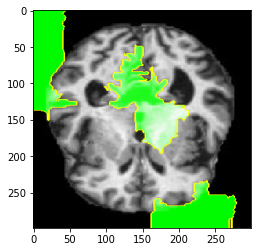
\includegraphics[width=\linewidth]{images/Non-demented.png}
        \caption{Interpretació de la categoria \textit{Non-demented} (I)}
        \label{fig:ND1}
    \end{subfigure}
    \begin{subfigure}[b]{0.40\linewidth}
        \raisebox{1.5cm}{
        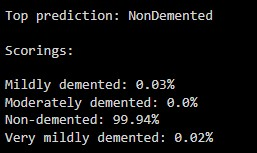
\includegraphics[width=\linewidth]{images/Non demented1.jpg}}
        \caption{Resultats numèrics de la categoria \textit{Non-demented} (I)}
        \label{fig:ClassificacioND1}
    \end{subfigure}
    \begin{subfigure}[b]{0.40\linewidth}
        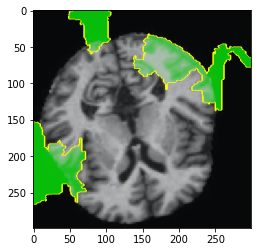
\includegraphics[width=\linewidth]{images/Non 2.png}
        \caption{Interpretació de la categoria \textit{Non-demented} (II)}
        \label{fig:ND2}
    \end{subfigure}
    \begin{subfigure}[b]{0.40\linewidth}
        \raisebox{1.5cm}{
        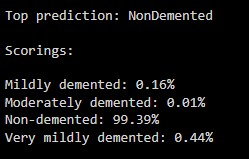
\includegraphics[width=\linewidth]{images/Non 2.1.jpg}}
        \caption{Resultats numèrics de la categoria \textit{Non-demented} (II)}
        \label{fig:ClassificacioND1}
    \end{subfigure}
    \caption{Interpretacions i resultats de classificació de la classe \textit{Non-demented}}
    \label{fig:NDInterpretacions}
\end{figure}

Com es pot observar en els resultats numèrics de la classificació, la xarxa neuronal està segura, quasi al 100\%, que les imatges utilitzades per fer la predicció corresponen a la classe \textit{Non demented}, atès que en ambdós casos els percentatges de classificació són superiors al 99\%.\\
En la interpretació gràfica feta amb la llibreria \textit{Lime}, es pot veure com la xarxa a més de fixar-se en parts interiors del cervell, també es fixa en parts de l'escorça cerebral, però en grau més baix i, finalment, també es fixa en parts que no corresponen al cervell. Com es pot saber a quines parts dona més importància la xarxa per fer una predicció? Per saber-ho solament cal parar compte amb els colors de la interpretació. El color verd indica un nivell d'importància molt elevat per la xarxa, el color groc indica un nivell d'importància mig i el color vermell un nivell d'importància baix.
\newpage
\textbf{Proves en la categoria \textit{Very-mild demented}}:
\begin{figure}[h!]
    \centering
    \begin{subfigure}[b]{0.40\linewidth}
        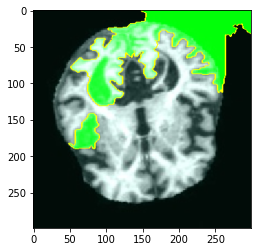
\includegraphics[width=\linewidth]{images/Very mildly.png}
        \caption{Interpretació de la categoria \textit{Very-mild demented} (I)}
        \label{fig:VMD1}
    \end{subfigure}
    \begin{subfigure}[b]{0.40\linewidth}
        \raisebox{1.5cm}{
        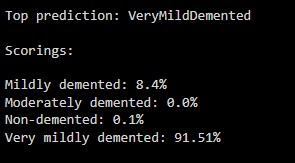
\includegraphics[width=\linewidth]{images/Very mildly1.jpg}}
        \caption{Resultats numèrics de la categoria \textit{Very-mild demented} (I)}
        \label{fig:ClassificacioVMD1}
    \end{subfigure}
    \begin{subfigure}[b]{0.40\linewidth}
        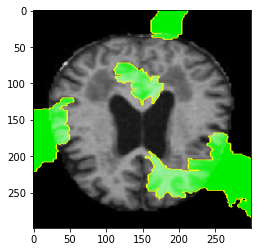
\includegraphics[width=\linewidth]{images/Very mild 2.png}
        \caption{Interpretació de la categoria \textit{Very-mild demented} (II)}
        \label{fig:VMD2}
    \end{subfigure}
    \begin{subfigure}[b]{0.40\linewidth}
        \raisebox{1.5cm}{
        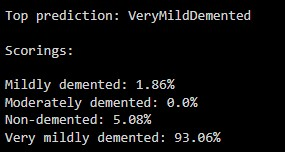
\includegraphics[width=\linewidth]{images/Very mild 2.1.jpg}}
        \caption{Resultats numèrics de la categoria \textit{Very-mild demented} (II)}
        \label{fig:ClassificacioVMD1}
    \end{subfigure}
    \caption{Interpretacions i resultats de classificació de la classe \textit{Very-mild demented}}
    \label{fig:VMDInterpretacions}
\end{figure}

En aquesta segona classe de classificació, \textit{Very-mild demented}, es pot observar un petit descens en els resultats numèrics de les classificacions, cosa que indica que la xarxa pot predir, de manera errònia, imatges de MRI d'aquesta categoria amb una mica més de facilitat.\\
En l'anàlisi de les interpretacions gràfiques, es pot observar un augment de les zones cerebrals a les quals, la xarxa, dona importància. En la imatge \ref{fig:VMD1} és on més es nota aquest augment de zones verdes. De la mateixa manera que en la categoria classificatòria anterior, es pot observar que la xarxa també dona importància a zones corresponents a l'escorça cerebral i, més o menys, si es compara, les zones importants de l'escorça del cervell són les mateixes.\\
\newpage
\textbf{Proves en la categoria \textit{Mild demented}}:\\
En aquesta ocasió, els percentatges de classificació tornen a enfilar-se cap als 99 alts, quasi arribant al 100\%, però si s'analitzen les interpretacions, es pot observar (sobretot en la imatge \ref{fig:MD1}), un augment significatiu de les zones negres com a zones importants per la xarxa (zones verdes). Cal remarcar que en la imatge \ref{fig:MD2} no hi ha, quasi, zones negres marcades com zones importants, però en altres proves aleatòries que s'han fet, l'augment de les zones negres s'ha pogut observar de manera empírica. Un altre aspecte que cal remarcar és que la xarxa també dona una importància molt alta a determinades zones de l'escorça cerebral per fer les prediccions.
\begin{figure}[h!]
    \centering
    \begin{subfigure}[b]{0.40\linewidth}
        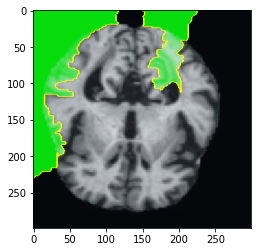
\includegraphics[width=\linewidth]{images/Mild.png}
        \caption{Interpretació de la categoria \textit{Mild demented} (I)}
        \label{fig:MD1}
    \end{subfigure}
    \begin{subfigure}[b]{0.40\linewidth}
        \raisebox{1.5cm}{
        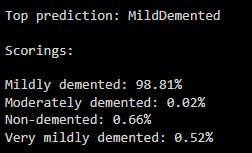
\includegraphics[width=\linewidth]{images/Mild1.jpg}}
        \caption{Resultats numèrics de la categoria \textit{Mild demented} (I)}
        \label{fig:ClassificacioMD1}
    \end{subfigure}
    \begin{subfigure}[b]{0.40\linewidth}
        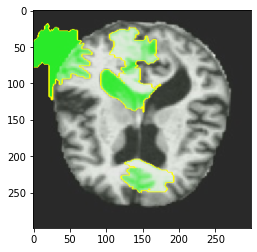
\includegraphics[width=\linewidth]{images/Mild 2.png}
        \caption{Interpretació de la categoria \textit{Mild demented} (II)}
        \label{fig:MD2}
    \end{subfigure}
    \begin{subfigure}[b]{0.40\linewidth}
        \raisebox{1.5cm}{
        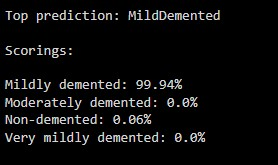
\includegraphics[width=\linewidth]{images/Mild 2.1.jpg}}
        \caption{Resultats numèrics de la categoria \textit{Mild demented} (II)}
        \label{fig:ClassificacioMD1}
    \end{subfigure}
    \caption{Interpretacions i resultats de classificació de la classe \textit{Mild demented}}
    \label{fig:MDInterpretacions}
\end{figure}
\newpage

\textbf{Proves en la categoria \textit{Moderate demented}}:
\begin{figure}[h!]
    \centering
    \begin{subfigure}[b]{0.40\linewidth}
        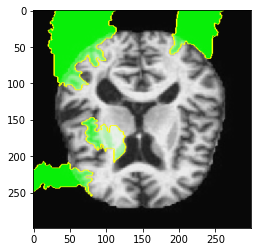
\includegraphics[width=\linewidth]{images/Moderately demented.png}
        \caption{Interpretació de la categoria \textit{Moderate demented} (I)}
        \label{fig:ModD1}
    \end{subfigure}
    \begin{subfigure}[b]{0.40\linewidth}
        \raisebox{1.5cm}{
        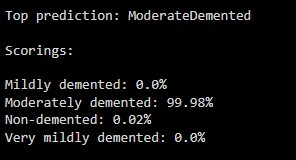
\includegraphics[width=\linewidth]{images/Moderately demented1.jpg}}
        \caption{Resultats numèrics de la categoria \textit{Moderate demented} (I)}
        \label{fig:ClassificacioModD1}
    \end{subfigure}
    \begin{subfigure}[b]{0.40\linewidth}
        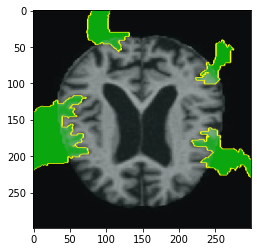
\includegraphics[width=\linewidth]{images/Moderate 2.png}
        \caption{Interpretació de la categoria \textit{Moderate demented} (II)}
        \label{fig:ModD2}
    \end{subfigure}
    \begin{subfigure}[b]{0.40\linewidth}
        \raisebox{1.5cm}{
        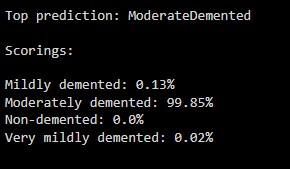
\includegraphics[width=\linewidth]{images/Moderate 2.1.jpg}}
        \caption{Resultats numèrics de la categoria \textit{Moderate demented} (II)}
        \label{fig:ClassificacioModD1}
    \end{subfigure}
    \caption{Interpretacions i resultats de classificació de la classe \textit{Moderate demented}}
    \label{fig:ModDInterpretacions}
\end{figure}
\newline
En aquest últim cas de classificació, es poden observar un altre cop prediccions fregant el 100\% en la classificació. En les interpretacions gràfiques s'observa un augment d'importància en zones de l'escorça cerebral que arriben a profunditzar una mica en la imatge del cervell.\\
Tot i que les zones negres quasi no són rellevants en la interpretació de les prediccions d'aquesta classe classificatòria, la importància d'aquestes zones continua present i, per tant, pot indicar una mala predicció que podria desembocar en un diagnòstic erroni si no es duen a terme les proves mèdiques pertinents.
\subsection*{Detalls tècnics d'implementació}
\addcontentsline{toc}{subsection}{Detalls tècnics d'implementació}
Abans de concloure aquesta secció del document cal que s'expliqui l'estructura del codi que s'ha seguit per implementar la proposta de treball des del preprocessament de les dades fins a la conversió del model en un format apte per la seva utilització en un futur sistema.\\
Com s'ha especificat anteriorment, el codi pertanyent a aquest treball de final de grau s'ha realitzat en una llibreta de \textit{Jupyter} a \textit{Google Drive}.\\
El primer pas, un cop carregat el \textit{dataset} a l'entorn de treball, és descomprimir-lo atès que solament es poden carregar fitxers comprimits. Per fer-ho es farà servir una comanda típica de línia de comandes (\textit{CMD}) del sistema operatiu.
\begin{lstlisting}
    !unrar x -Y "content/dataset.rar" "/content/"
\end{lstlisting}
El signe d'exclamació, és un indicador, com s'ha esmentat abans, que aquesta comanda és una comanda que s'executa en una \textit{CMD}. La \textit{option} \texttt{x} indica a la comanda que es vol extreure el fitxer del qual s'especifica el \textit{path} complet. La \textit{flag} \texttt{-Y} indica que durant la descompressió, se sobreescriuran totes les dades a la ruta de destinació.\\
Seguidament, s'instal·la la dependència necessària per poder fer una interpretació de les prediccions que fa el model un cop aquest estigui entrenat.\\
Un cop les dades estan descomprimides, les dependències instal·lades i importades i les rutes als fitxers d'entrenament i validació definides, cal definir una sèrie de paràmetres com les dimensions de les imatges, el nombre de classes de classificació, el nombre d'èpoques que s'entrenarà el model, el paràmetre \textit{batch\_size} i caldrà posar en una llista els noms de les etiquetes. A continuació es mostra un exemple del fragment de codi.
\begin{lstlisting}
    width_shape = 200
    height_shape = 190
    num_labels = 4
    epochs = x
    batch_size = y
    label_names = ["MildDemented", "ModerateDemented", "NonDemented", "VeryMildDemented"]
\end{lstlisting}
on,
    \[epochs = \{x \mid x \in \mathbf{N} \land x > 0 \}\]
    \[batch\_size = \{y \mid y \in \mathbf{N} \land y > 0 \}\]
A continuació es creen dos \textit{ImageDataGenerator()}. Un per l'entrenament i l'altre per a la validació. En aquests \textit{ImageDataGenerator()} s'introdueixen les dades de les imatges del directori que correspongui. Aquestes dades són un total de sis: la ruta al directori, les mides, la \textit{batch\_size}, el color, el \textit{class\_mode} i el booleà de mescla.\\
Quan ja estan els paràmetres definits i les imatges preprocessades, arriba el moment de configurar el model.\\
El model està definit amb una arquitectura seqüencial per tres raons. La primera és que un model d'arquitectura lineal permet una major flexibilitat que un model d'arquitectura convolucional. És a dir, el fet d'utilitzar diferents tipus de capes, permet construir models complexos i, si s'escau, adaptar-los a altres tasques que no siguin la classificació. La segona raó, és la capacitat de processar seqüències. És a dir, aquests tipus de models són molt útils per dur a terme tasques de processament de seqüències, com per exemple, el reconeixement de veu. La utilització de capes convolucionals, juntament amb altres tipus de capes especialitzades a processar seqüències, dona com a resultat un model capaç d'extreure patrons en els seus \textit{inputs}. La tercera, i última, raó per la qual l'arquitectura del model és seqüencial és la reducció de la complexitat. Els models d'arquitectura convolucional, necessiten molts paràmetres cosa que desemboca en una complexitat elevada, un temps d'entrenament molt prolongat i un major risc d'\textit{overffiting}. Els models seqüencials redueixen aquesta complexitat gràcies a l'ús de les capes de \textit{pooling}. L'ús d'aquestes capes no solament redueix la complexitat del model, sinó que també redueix el temps d'entrenament i millora el rendiment del model.\\
Un cop definida l'arquitectura, es van afegint les diferents capes de convolució, de normalització, de \textit{pooling} i de regularització. Aquesta combinació de capes es realitza quatre cops i seguidament s'afegeix una capa d'aplanament seguida d'una capa densa, una de normalització, una d'activació, una de regularització i una classificació també densa. Per tant, la construcció del model queda de la següent manera:
\begin{lstlisting}
    model = Sequential()

    # Convolutional layer 1
    model.add(Conv2D(32, kernel_size=(3, 3), pading="same", activation="relu", strides=1, input_shape=(width_shape, height_shape, 1)))
    model.add(BatchNormalizartion())
    model.add(MaxPool2D(pool\_size=(2, 2)))
    model.add(Dropout(0.2))

    # Convolutional layer 2
    model.add(Conv2D(64, kernel_size=(5, 5), padding="same", activation="relu", strides=1))
    model.add(BatchNormalizartion())
    model.add(MaxPool2D(pool_size=(2, 2)))
    model.add(Dropout(0.2))

    # Convolutional layer 3
    model.add(Conv2D(128, kernel_size=(3, 3), padding="same", activation="relu", strides=1))
    model.add(BatchNormalizartion())
    model.add(MaxPool2D(pool_size=(2, 2)))
    model.add(Dropout(0.2))

    # Convolutional layer 4
    model.add(Conv2D(256, kernel_size=(5, 5), padding="same", activation="relu", strides=1))
    model.add(BatchNormalizartion())
    model.add(MaxPool2D(pool_size=(2, 2)))
    model.add(Dropout(0.2))

    model.add(Flatten())

    # Dense layer
    model.add(Dense(1024))
    model.add(BatchNormalizartion())
    model.add(Activation("relu"))
    model.add(Dropout(0.2))

    # Classification layer
    model.add(Dense(num_labels, activation="softmax"))
\end{lstlisting}
El fet d'utilitzar la funció d'activació \textit{relu} en les capes que no fan la classificació i la funció \textit{softmax} en la capa de classificació té un sentit. Per la manera de treballar que tenen ambdues funcions d'activació, és pot concloure que l'ús de la funció \textit{relu} en les capes no classificatòries ajuda a aprendre les diferents representacions complexes que tenen les dades. L'ús de la funció \textit{softmax} en la capa que realitza la classificació, proporciona com \textit{output} una distribució de probabilitats, és a dir, aquesta funció proporciona una repartició de les probabilitats, que té una entrada, a pertànyer a una de les classes de classificació.\\
Si es desitja obtenir més informació de les funcions \href{https://machinelearningmastery.com/rectified-linear-activation-function-for-deep-learning-neural-networks/}{\underline{\textit{relu}}} i \href{https://interactivechaos.com/es/manual/tutorial-de-machine-learning/regresion-softmax}{\underline{\textit{softmax}}}, consultar els enllaços proporcionats.
En aquest punt, el model ja està definit i llest per la compilació i l'entrenament, per tant, en primer lloc, es compilarà el model amb la crida \textit{model.compile()} i l'optimitzador Adam. Aquest optimitzador combina les propietats dels optimitzadors de descens de gradient estocàstic (SGD) i de l'estimador adaptatiu de moments (RMSProp). Adam, en primer lloc, inicialitza una taxa d'aprenentatge i els pesos inicials del model intel·ligent. Seguidament, realitza el càlcul dels gradients (necessàri per aplicar els pesos a les neurones) del model basant-se en la funció de pèrdua utilitzant la tècnica de retropropagació. El funcionament d'aquesta tècnica costa de quatre passos bàsics:
\begin{enumerate}
    \item La capa d'entrada rep l'\textit{input} que ha de ser processat.
    \item Els pesos de les connexions interneuronals s'inicialitzen de manera aleatòria a menys que s'especifiqui algun mètode concret.
    \item Les capes ocultes del model processen la sortida de l'element que s'ha entrat al pas 1. Les sortides s'anomenen "Error" i són la diferència entre la sortida real i la sortida del model.
    \item L'algorisme torna cap enrere a les capes ocultes i optimitza els pesos interneuronals per reduir la dimensió de l'error.
\end{enumerate}
Quan la tècnica de retropropagació ja ha estat aplicada, el següent pas és calcular la mitjana mòbil del gradient i el gradient al quadrat. El quart pas és calcular les mitjanes mòbils corregides pel biaix. Per biaix s'entén la tendència que té el model a fer suposicions sobre una entrada.\\
El cinquè i últim pas de treball de l'optimitzador Adam, es actualitzar els pesos del model utilitzant el càlcul del pas anterior.\\
Amb la crida a la funció \textit{model.fit()} es duu a terme l'entrenament del model.\\
Després d'entrenar el model, mitjançant una crida a la funció \textit{model.evaluate()} es treu per pantalla tant la precisió del model com la seva pèrdua. Cal remarcar que la funció de pèrdua utilitzada és \textit{categorical crossentropy}, atès que s'està portant a cap una tasca de classificació multiclasse.\\
Tot seguit es realitza un test amb una imatge aleatòria. Per dur a terme aquest test se selecciona una imatge, aleatòria i, abans de fer la predicció es fan un seguit d'operacions per adaptar la imatge al format que el model espera.
\begin{lstlisting}
    test_brains = []
    pic_path = "path/to/image"
    test_brain = cv2.cvtColor(cv2.imread(pic_path), cv2.COLOR_BGR2GRAY)
    test_brain = cv2.resize(test_brain, (190, 200))
    test_brain2 = img_to_array(test_brain)
    test_brain2 = np.expand_dims(test_brain2, axis=0)
    test_brains.append(test_brain2)
    prediction = model.predict(test_brains)
    print("Top prediction; " + label_names[np.argmax(prediction)] + "\n"]
    percentages = []
    for i in range(0, len(prediction[0])):
        percentages.append(round(prediction[0][i] * 100, 2))
    print("Scorings: " + "\n")
    print("Mildly demented: " + str(percentages[0] + "%")
    print("Moderately demented: " + str(percentages[1] + "%")
    print("Non-demented: " + str(percentages[2] + "%")
    print("Very mildly demented: " + str(percentages[3] + "%")
\end{lstlisting}
Primerament, la imatge seleccionada es converteix en una imatge en escala de grisos. En segon lloc, es redimensiona a les mides esperades pel model. Seguidament, es transforma la imatge en un \textit{numpy-array} perquè el model la pugui processar. La quarta operació que es realitza abans de fer la predicció és afegir una nova dimensió en la posició 0 del \textit{numpy-array} (axis = 0) que prendrà per valor el de la \textit{batch\_size} atès que el model espera una entrada del tipus: (\textit{batch\_size}, \textit{height}, \textit{width}, \textit{channels}), on el paràmetre \textit{channels} és un identificador que especifica si la imatge és en blanc i negre (1) o en color (3). Un cop fetes totes aquestes operacions, la imatge de test ja està adaptada al tipus d'entrada que espera el model i, per tant, ja es pot fer la predicció. Finalment, es treu per pantalla la predicció més elevada, juntament amb el tant per cent. A més de treure la predicció més alta, també es treuen per pantalla la resta de les possibles classificacions juntament amb els tant per cent que la xarxa els hi ha atorgat.
Finalment, abans de guardar el model en un fitxer per la seva posterior integració en un sistema, per tenir una mica més clar com fa les prediccions el model s'utilitza la llibreria \textit{Lime} per obtenir una interpretació gràfica de les prediccions.\\
Aquest pas es basa en, un cop creat l'explicador, preprocessar l'entrada de la qual es vol obtenir l'explicació realitzar i realitzar la predicció tot aplicant una màscara desitjada. Per fer obtenir l'explicació s'usarà la funció \textit{explain\_instance()} i per obtenir la imatge amb la màscara s'usarà la funció \textit{get\_image\_and\_mask()} El resultat es veurà com les imatges \ref{fig:NDInterpretacions}, \ref{fig:VMDInterpretacions}, \ref{fig:MDInterpretacions} i \ref{fig:ModDInterpretacions}.\\
\newline
Finalment, el model es guardarà en un fitxer \textit{.h5} que servirà per integrar-lo en un sistema. Aquest tipus de fitxer guarda totes les dades necessàries del model per poder-lo utilitzar en un futur.
\chapter*{Conclusions}
\addcontentsline{toc}{chapter}{Conclusions}
Per concloure aquesta investigació, cal presentar quines conclusions s'han extret d'aquesta durant aquest període de quasi un any de feina.\\
La primera de les conclusions és, que la malaltia d'Alzheimer és una malaltia molt més comuna del que una persona es pot pensar i que tot i tenir una llarga història d'investigació i dures batalles per trobar-ne totes les causes, en ple segle XXI després de més de cent anys del seu descobriment, aquesta malaltia continua sent una gran desconeguda en alguns aspectes referents a factors condicionants a patir-la.\\
La segona conclusió, és que tot i que des de l'any 1901 s'ha avançat molt en la lluita contra l'Alzheimer, encara no hi ha cap medicina específica per tractar la malaltia, solament hi ha medicines per tractar els símptomes.\\
Com a tercera conclusió s'extreu que, tant l'herència genètica com l'estil de vida són factors molt importants per saber si una persona té un risc superior, al de la resta de la població, de patir Alzheimer.\\ 
La quarta conclusió extreta d'aquesta recerca és que tot i haver tingut familiars amb aquesta malaltia, els símptomes del cas familiar són solament una petita gota en l'estany que representa el conjunt de símptomes.\\
La conclusió número cinc és que el món de la medicina coneix bastant bé com evoluciona la malaltia i, per tant, sap dividir les diferents etapes de la malaltia segons el dany cerebral que presenta la persona.\\
En sisè lloc, cal remarcar que el procés de diagnosi de la malaltia és un procés llarg i complex atès que cal realitzar moltes proves i estudis abans d'establir l'Alzheimer com a diagnòstic final d'un pacient.\\
Abandonant les conclusions clíniques i començant a abordar les conclusions computacionals, la setena conclusió que es pot extreure d'aquesta recerca és que el senyor Alan Turing, a més d'establir les bases informàtiques sense les quals molts aspectes, com la IA, de la informàtica actual no serien possibles. Sense saber-ho, Alan Turing va establir les bases d'una tècnica (la intel·ligència artificial) que avui dia s'utilitza, de manera experimental, per la diagnosi no solament de l'Alzheimer sinó d'altres afeccions com el càncer.\\
La vuitena conclusió és que gràcies a grans informàtics com \textit{Stuart Russell} i \textit{Peter Norvig}, les bases que va assentar el senyor Turing sobre la intel·ligència artificial, han pogut ser desenvolupades profundament, dividides en categories i millorades.\\
La conclusió número deu és que la IA té molts avantatges i facilita i accelera molts processos que als humans ens porten un determinat temps i un determinat esforç mental. Tot i que aquesta tècnica de voler reproduir la intel·ligència humana en màquines té una part bona molt extensa, també té la seva part fosca i existeix la possibilitat futura que quan els sistemes intel·ligents desenvolupin una consciència pròpia, els humans siguem incapaços de controlar aquests sistemes.\\
L'onzena conclusió és que per molt que una persona tingui coneixements sobre un tema concret, mai es té prou saber per a dur a terme una investigació sense trobar-se amb algun repte pel camí. En el cas d'aquesta investigació es poden observar els reptes trobats en la següent secció d'aquest document.\\
En dotzè lloc, es pot extreure la conclusió que de vegades és més senzill interpretar els resultats d'un experiment determinat de manera gràfica que de manera numèrica. En el cas d'aquesta recerca, fins que no s'han observat, de manera gràfica, les dades resultants dels entrenaments dels diferents experiments, no s'ha pogut assegurar quines versions dels models estaven en situació d'\textit{overffiting}.\\
Seguint amb les conclusions de la part computacional d'aquest treball de final de grau, la tretzena, i penúltima, conclusió extreta, és que un petit canvi en algun dels paràmetres del model, siguin hiperparàmetres, un canvi del conjunt de dades, un canvi de les funcions d'activació de les capes, un canvi en el nombre de filtres de les capes convolucionals, etc., comporta un canvi notable en el rendiment final del model.\\
La catorzena, i última, conclusió, és referent a les interpretacions de les prediccions amb Lime. Com s'ha comentat amb anterioritat, hi ha algunes imatges en les quals, la xarxa neuronal, pren com a importants zones negres que res tenen a veure amb la imatge del cervell, per tant, això és un aspecte que caldria corregir en futures implementacions, i encara s'hauria de corregir amb més precisió si aquest model intel·ligent s'hagués d'utilitzar en els hospitals. En conseqüència, tot i que moltes de les zones que es prenen com a rellevants són correctes (són zones del cervell) caldria continuar corregint el model fins que les interpretacions indiquin que no es prenen zones negres com a zones importants.
\chapter*{Reptes i dificultats durant la realització del TFG}
\addcontentsline{toc}{chapter}{Reptes i dificultats durant la realització del TFG}
La realització d'aquesta investigació no ha estat del tot fàcil atès que s'ha hagut de batallar amb alguns problemes tant pel que fa a informació teòrica, com a escala d'implementació com en l'àmbit de redacció.\\
En l'àmbit de la cerca d'informació el principal repte ha estat el contrast de la informació que s'anava trobant. Ha estat una dificultat perquè a la xarxa hi ha molta informació sobre un mateix tema, molt variada i, de vegades, contradictòria. Per tant, el contrast de tota la informació que s'anava cercant era molt important per assegurar-se de no donar com a informació verídica quelcom que no és veritat.\\
La part d'implementació, tot i els meus coneixements previs sobre aprenentatge automàtic, també ha estat un repte important, instructor però, per sobre de tot, bonic. Els meus coneixements previs de \textit{Machine Learning} eren bastant limitats pel que fa a xarxes convolucionals i, conseqüentment, no coneixia del tot bé com funcionava l'estructura d'aquesta arquitectura. Gràcies a la xarxa i als meus amics ha estat possible conèixer prou per a culminar amb èxit aquest estudi.\\
Una altra dificultat d'implementació de la proposta ha estat la llibreria \textit{Lime}. Aquesta llibreria era una completa desconeguda per mi. Per tant, després d'una lectura, a fons, de la documentació i de veure alguns exemples de codi la integració d'aquest mètode per interpretar les prediccions del model ha estat senzilla.\\
Finalment, l'últim dels reptes més grans ha estat en el moment de la redacció de la memòria en LaTeX. Tot i els meus amplis, però no en excés, del llenguatge de redacció de documents m'he anat trobant alguns problemes en relació amb, per exemple, la representació gràfica de dades, la introducció de dues imatges en una sola figura, l'adheriment d'un document PDF (la plantilla portada) al document LaTeX i tenir una sèrie d'índexs (continguts, figures i taules) que superen la pàgina.\\
L'últim problema amb què m'he topat, tot i ser un problema de menor calibre, és un problema important. El problema era la correcta redacció d'una referència bibliogràfica (referència a un llibre). Desconeixia si hi ha alguna metodologia específica per fer-ho. Ara ja sé que l'ordre correcte és: autor/a, títol, publicador, any.
\chapter*{Glossari}
\addcontentsline{toc}{chapter}{Glossari}
\section*{Glossari I: Síndrome plurietològic}
\addcontentsline{toc}{section}{Glossari I: Síndrome plurietològic}
Una síndrome és un conjunt de símptomes amb personalitat clínica acusada. És a dir, és un grup de símptomes o afeccions que es presenten de manera conjunta en un individu i que suggereixen la presència d'una certa malaltia o una major probabilitat de patir una malaltia. Una síndrome és plurietològic quan els símptomes o afeccions que la caracteritzen poden ser produïdes per diverses causes. Gràcies a aquestes diverses causes, es poden diferenciar les formes primàries i secundàries d'un mateix síndrome. Les formes primàries són aquelles síndromes que no es poden relacionar amb cap afecció coneguda, mentre que les formes secundàries, són aquelles síndromes que estan vinculades, com a mínim, a una malaltia coneguda.
\section*{Glossari II: Acetilcolina}
\addcontentsline{toc}{section}{Glossari II: Acetilcolina}
L'acetilcolina és una substància química que elaboren algunes neurones. Aquesta substància serveix per enviar missatges a altres cèl·lules. S'allibera per la terminació del nervi i porta senyals a les cèl·lules que estan a l'altra banda d'una sinapsi (espai entre les cèl·lules nervioses i altres cèl·lules). Aquesta substància ajuda a controlar la memòria i l'accionat de certs músculs. L'acetilcolina fou el primer neurotransmissor descobert.
\section*{Glossari III: Arrítmia cardíaca}
\addcontentsline{toc}{section}{Glossari III: Arrítmia cardíaca}
Una arrítmia cardíaca o arrítmia és un trastorn de la freqüència cardíaca (pols) o del ritme cardíac. Aquest trastorn té dues variants diferents. El primer és la taquicàrdia que és quan el cor batega massa ràpid, i el segon és la bradicàrdia que és quan el cor batega massa lent o de manera irregular.
\section*{Glossari IV: Neurotransmissor}
\addcontentsline{toc}{section}{Glossari IV: Neurotransmissor}
Els neurotransmissors són les substàncies que utilitzen les neurones per poder comunicar-se entre elles i per poder-se comunicar amb altres teixits sobre els quals actuaran en el procés de sinapsi. Els neurotransmissors se sintetitzen i s'alliberen a les terminacions nervioses a l'altura de l'espai sinàptic. Després de la seva alliberació, es lliguen a diferents proteïnes a la membrana cel·lular del teixit diana i aquest pot excitar-se, inhibir-se o modificar-se funcionalment.
\section*{Glossari V: FDA}
\addcontentsline{toc}{section}{Glossari V: FDA}
FDA són les sigles de l'administració d'aliments i fàrmacs dels Estats Units (\textit{Food and drug administration} en anglès). La FDA és la màxima autoritat sanitària del país i s'encarrega de la regularització d'aliments, medicines (humanes i veterinàries), cosmètics, vacunes, etc. Per tant, si s'engloba tot en un sol grup, es podria dir que la FDA és l'organització governamental encarregada de vetllar per la salut pública.
\section*{Glossari VI: Glutamat}
\addcontentsline{toc}{section}{Glossari VI: Glutamat}
El glutamat és una substància que utilitzen moltes empreses per potenciar el sabor dels aliments i que en el cos humà actua com un neurotransmissor excitador. A més de ser el neurotransmissor més abundant del cervell d'un animal vertebrat, és el neurotransmissor que s'utilitza en totes les funcions importants del cervell i representa un 90\% de les connexions sinàptiques del cervell humà.
\section*{Glossari VII: Proteïna beta-amiloide}
\addcontentsline{toc}{section}{Glossari VII: Proteïna beta-amiloide}
La proteïna beta-amiloide és un aminoàcid d'entre 36 i 43 aminoàcids de llarg processat a partir d'un precursor de la proteïna amiloide, que és una proteïna transmembrana. És la principal component de les plaques senils i, per tant, tot i que aquesta proteïna es produeix de manera natural en el cervell, l'acumulació en forma de plaques amiloides és un dels moduladors de l'Alzheimer.
\section*{Glossari VIII: Edema cerebral}
\addcontentsline{toc}{section}{Glossari VIII: Edema cerebral}
Un edema cerebral és una inflamació del teixit tou cerebral provocada per una acumulació de líquid en les cèl·lules cerebrals. Aquest trastorn causa un augment de la pressió intracranial, cosa que desemboca en una falta d'oxigenació i degeneració cel·lular que pot provocar la mort.
\section*{Glossari IX: Hemosiderina}
\addcontentsline{toc}{section}{Glossari IX: Hemosiderina}
L'hemosiderina és un pigment (material que canvia el color de la llum que reflecteix) groguenc i d'aspecte granulós que deriva de l'hemoglobina quan hi ha un excés de ferro al cos.
\section*{Glossari X: MRI}
\addcontentsline{toc}{section}{Glossari X: MRI}
MRI són les sigles en anglès de \textit{Magnetic Resonance Imaging}, que significa imatge per ressonància magnètica. Un MRI és una tecnologia de presa d'imatges anatòmiques detallades tridimensionals. És un procediment no invasiu utilitzat per la detecció de malalties, diagnosi i monitoratge de tractaments. Es basa en una sofisticada tecnologia que excita i detecta el canvi de direcció de l'eix de rotació dels protons que es troben a l'aigua que formen els teixits.
\section*{Glossari XI: Historial clínic}
\addcontentsline{toc}{section}{Glossari XI: Historial clínic}
L'historial clínic d'un pacient és un conjunt de documents relatius als processos assistencials d'aquell pacient on s'identifiquen els metges i altres professionals que han intervingut en els diferents processos. L'objectiu d'un historial clínic és obtenir la màxima integració possible de la documentació clínica de cada pacient.
\section*{Glossari XII: Emil Kraepelin}
\addcontentsline{toc}{section}{Glossari XII: Emil Kraepelin}
El Dr. Kraepelin va ser un psiquiatre alemany que va viure entre finals del segle XIX i principis del XX. La seva manera d'entendre les malalties mentals basant-se en conceptes científics naturals va tenir un gran impacte en la psiquiatria actual. De fet, el Dr. Kraepelin és considerat el pare de la psiquiatria científica moderna, la psicofarmacologia i la genètica psiquiàtrica.\\
Una de les aportacions més importants del doctor al món de la psiquiatria va ser la identificació i distinció del trastorn maniàtic depressiu i de la demència precoç (més tard anomenada esquizofrènia). Va considerar que la depressió maníaca era un trastorn episòdic no neurodegeneratiu mentre que l'esquizofrènia provocava un deteriorament cognitiu permanent. El Dr. Kraepelin va establir que la diferència entre aquestes dues formes de psicosi es trobava en el patró dels símptomes i no en la semblança.
\section*{Glossari XIII: Espaitemps}
\addcontentsline{toc}{section}{Glossari XIII: Espaitemps}
El terme espaitemps fou usat per primer cop l'any 1908 pel matemàtic alemany Hermann Minkowski. Aquest terme fusiona els termes newtonians absoluts de l'espai i del temps en un nou constructe tetradimensional on les tres primeres dimensions eren les tres dimensions ordinàries de l'espai i la quarta dimensió representava el temps.\\
En la concepció original, el temps, és geomètricament pla, però matemàticament és bastant curiós perquè, el temps, es comporta com una coordenada espacial però amb valors complexos. Gràcies a la teoria de la relativitat general d'Einstein que introduí l'efecte gravitacional, va sorgir la suposició que l'espaitemps de Minkowski no era pla, sinó que estava corbat.
\section*{Glossari XIV: Autòpsia}
\addcontentsline{toc}{section}{Glossari XIV: Autòpsia}
Una autòpsia és l'examinació detallada d'unes restes mortals. Aquest procés pot servir per múltiples aspectes com esbrinar quelcom sobre una malaltia o lesió o, també, per esbrinar com i per què ha mort la persona a la qual se li practica aquest procediment.\\
Les autòpsies les duen a terme metges especialitzats anomenats patòlegs forenses que són experts en examinar teixits i líquids corporals, cosa que els permet interpretar descobriments post-mortem i recopilar dades forenses sobre la mort d'aquella persona en els casos de mort violenta o sospitosa. Normalment, treballen juntament amb altres especialistes com toxicòlegs o antropòlegs forenses per esbrinar de manera precisa les causes de la mort d'una persona.
\section*{Glossari XV: Proteïna Tau}
\addcontentsline{toc}{section}{Glossari XV: Proteïna tau}
Juntament amb la proteïna beta-amiloide (anteriorment descrita) són dues proteïnes directament relacionades amb l'Alzheimer que tenen quatre funcions principals. La primera és mantenir l'estructura micro tubular. El micro tubs són unes estructures que es troben a l'interior de les cèl·lules, a través de les quals es transmet la informació i es permet el moviment dels axons (estructures nervioses que transmeten els impulsos nerviosos entre les cèl·lules nervioses) de les neurones. La segona funció que tenen és participar en la formació de noves neurones (procés anomenat neurogènesi). La tercera funcionalitat és la regulació dinàmica micro tubular i, la quarta i última funcionalitat és protegir contra la degeneració neuronal i la mort cel·lular.
\section*{Glossari XVI: Biomedicina}
\addcontentsline{toc}{section}{Glossari XVI: Biomedicina}
La biomedicina és una disciplina que aplica tècniques de l'enginyeria a les ciències de la vida. La biomedicina es dedica principalment al dissenyat i construcció d'eines i tecnologia com, per exemple, equipaments mèdics, pròtesis, dispositius de teràpia, etc. També es pot dedicar a estudiar i preparar dissenys d'equips electrònics per a hospitals, imatges de raigs X, etc.\\
La biomedicina té la capacitat de fer que els metges, a més de ser metges, siguin també científics gràcies a la incorporació de coneixements en matèries de química, biologia, física i matemàtiques.\\
Els tres elements que units resulten en la biomedicina són: l'enginyeria informàtica i les ciències de la computació per al processament de dades, l'enginyeria electrònica per a poder desenvolupar circuits electrònics per a l'adquisició de dades i així, juntament amb la informàtica, crear solucions \textit{hardware} i \textit{software} i, per últim, el tercer pilar de la biomedicina són les ciències de la vida (ciències que estudien els éssers vius).
\section*{Glossari XVII: APOE E-4}
\addcontentsline{toc}{section}{Glossari XVII: APOE E-4}
E-4 és una versió del gen APOE que incrementa el risc individual d'un ésser humà de desenvolupar, de manera tardana, la malaltia d'Alzheimer.\\
El gen APOE proporciona instruccions per fer una proteïna anomenada apolipoproteïna E. Aquesta proteïna es combina amb els greixos del cos per formar molècules anomenades lipoproteïnes i aquestes són les que s'encarreguen de transportar el colesterol i altres grasses pel sistema circulatori.\\
Existeixen, com a mínim tres versions (al·lels) d'aquest gen. Els principals s'anomenen E2, E3 i E4 sent l'E3 el més comú.
\section*{Glossari XVIII: Gen}
\addcontentsline{toc}{section}{Glossari XVIII: Gen}
Els gens són considerats la unitat bàsica de l'herència que passa de pares a fills. Els gens són segments de l'ADN d'una persona; la majoria dels gens contenen informació per elaborar una proteïna específica o segments de proteïnes, que tenen diferents funcionalitats en el cos de les persones. En ells també es pot trobar la informació necessària per determinar característiques físiques i biològiques d'una persona com el seu gènere, color de pell, color d'ulls i informació que predisposi a una persona a patir una malaltia, entre altres informacions variades.
\section*{Glossari XIX: Mutació genètica}
\addcontentsline{toc}{section}{Glossari XIX: Mutació genètica}
Una mutació genètica és un canvi en un o més gens podent, algun d'aquests canvis, provocar diferents malalties. És a dir, una mutació genètica és una alteració en la seqüència de l'ADN.
\section*{Glossari XX: Traumatisme cranial}
\addcontentsline{toc}{section}{Glossari XX: Traumatisme cranial}
Un traumatisme cranial és qualsevol traumatisme (lesió produïda per un cop amb un objecte contundent)
 que es produeix al cuir cabellut, el crani o el cervell. Existeixen dos tipus de traumatismes cranials. El traumatisme cranial tancat, que és aquell en què l'impacte no arriba a trencar el crani i el traumatisme cranial obert que és aquell en què el cop arriba a trencar el crani i penetra fins al cervell.
\section*{Glossari XXI: Desordre neurodegeneratiu}
\addcontentsline{toc}{section}{Glossari XXI: Desordre neurodegeneratiu}
Un desordre neurodegeneratiu és una malaltia en la qual les cèl·lules del cervell i la mèdula espinal deixen de funcionar o moren. Normalment, aquests trastorns van a pitjor amb el pas del temps i no tenen cura. Hi ha tres factors, naturals, que els poden causar: herència genètica, tumors o els ictus. Tabé poden ser causats per factor artificials com l'alcoholisme i l'exposició a virus i toxines.
\section*{Glossari XXII: Simptomatologia}
\addcontentsline{toc}{section}{Glossari XXII: Simptomatologia}
S'anomena simptomatologia a un conjunt de síntomes que quan es manifesten tots junts es relacionen amb una dolència. Un simptoma és una manifestació indicadora d'una malaltia.
\section*{Glossari XXIII: Demència vascular}
\addcontentsline{toc}{section}{Glossari XXIII: Demència vascular}
La demència vascular és la segona causa de demència després de l'Alzheimer, suposant entre un 15\% i un 20\% dels casos totals diagnosticats de demència.\\
Aquest tipus de demència és el resultat de diverses afeccions, com per exemple, els ictus que interrompen el flux sanguini que va cap al cervell. Aquest fet desemboca en problemes amb la memòria, el pensament, el raonament i el comportament. La característica principal d'aquesta demència és que pot desenvolupar-se tota sola o juntament amb algun altre tipus de demència, per tant, seria perfectament possible ser diagnosticat amb demència vascular i Alzheimer.
\section*{Glossari XXIV: Demència amb cossos de Lewy}
\addcontentsline{toc}{section}{Glossari XXIV: Demència amb cossos de Lewy}
La demència amb cossos de Lewy causa un deteriorament, progressiu, de les capacitats mentals. Les persones que són diagnosticades amb aquesta demència, podent patir al·lucinacions visuals, canvis en l'atenció i moments de confusió (disminució de la lucidesa mental). Altres símptomes poden ser la rigidesa muscular, lentitud de moviments i tremolor.\\
Aquesta demència es desenvolupa quan els dipòsits de proteïnes, anomenades cossos de Lewy, es desenvolupen en les cèl·lules de les regions cerebrals que tenen el control motor del cos.
\section*{Glossari XXV: Demència frontotemporal}
\addcontentsline{toc}{section}{Glossari XXV: Demència frontotemporal}
La demència frontotemporal és un grup de trastorns que afecten els lòbuls frontal i temporal del cervell. Aquestes dues àrees del cervell són les associades amb la personalitat, la conducta i la parla.\\
En aquest tipus de demència, aquests lòbuls s'atrofien i, per tant, els símptomes varien segons quina és la regió del lòbul atrofiada.\\
Alguns dels símptomes poden ser: canvis dramàtics en la personalitat, desenvolupar una conducta socialment inapropiada, impulsivitat, perdre la capacitat d'utilitzar correctament una llengua.\\
Aquesta demència pot ser confosa amb l'Alzheimer, però hi ha un factor que decanta la balança cap a la demència frontotemporal, l'edat. Aquesta demència tendeix a aparèixer en edats més primerenques que l'Alzheimer. Aproximadament entre un 10\% i un 20\% dels casos de demència són casos de demència frontotemporal.
\section*{Glossari XXVI: Demència mixta}
\addcontentsline{toc}{section}{Glossari XXVI: Demència mixta}
La demència mixta és un tipus de demència que es caracteritza per presentar símptomes típics de més d'un tipus de demència. Sovint solen ser l'Alzheimer i la demència vascular. De vegades també hi poden haver símptomes de demència amb cossos de Lewy.
\section*{Glossari XXVII: Deteriorament cognitiu}
\addcontentsline{toc}{section}{Glossari XXVII: Deteriorament cognitiu}
El deteriorament cognitiu són les alteracions que té una persona en el seu pensament, la seva capacitat per aprendre, la memòria, el judici i la presa de decisions. Els senyals que indiquen que una persona pateix aquesta afecció són la pèrdua de memòria, la dificultat per mantenir la concentració, completar activitats, comprendre, seguir unes instruccions, solucionar problemes de la vida quotidiana, canvis conductuals, pèrdua de motivació i desorientació. Algunes de les causes més comunes que provoquen el deteriorament cognitiu són el càncer i alguns dels seus tractaments.
\section*{Glossari XXVIII: Dieta mediterrània}
\addcontentsline{toc}{section}{Glossari XXVIII: Dieta mediterrània}
La dieta mediterrània és una dieta amb una menor quantitat de carns i carbohidrats que una dieta típica dels Estats Units. També té més quantitat de vegetals i greixos monoinsaturats (greixos bons).\\
Seguir una dieta d'estil mediterrani pot suposar una estabilització dels nivells de sucre en sang, una disminució del colesterol i dels triglicèrids i un menor risc al desenvolupament d'afeccions cardíaques.
\section*{Glossari XXIX: Dieta DASH}
\addcontentsline{toc}{section}{Glossari XXIX: Dieta DASH}
La dieta DASH és una dieta baixa en sal i alta en fruites, verdures, grans integrals i làctis baixos en greixos i proteïnes magres. La paraula DASH són unes sigles que corresponen a \textit{Dietary Approaches to Stop Hypertension}, que en català significa: "Enfocaments alimetàris per parar la hipertensió". Aquesta dieta es va crear, originalment, per ajudar a aquelles persones amb hipertensió a a reduir la pressió arterial. També és una manera saludable de perdre pes.
\section*{Glossari XXX: Metge de capçalera}
\addcontentsline{toc}{section}{Glossari XXX: Metge de capçalera}
El metge de capçalera és un metge pertanyent a l'atenció primària d'un sistema de salut públic que atèn a les persones amb dolències comunes. Normalment, un metge de capçalera és una persona amb una titulació de medicina, però, també pot ser un assistent mèdic o una persona que sigui professional de l'infermeía. El metge de capçalera és qui donarà tractaments als pacients durant un període de temps prolongat.
\section*{Glossari XXXI: Diagnòstic diferencial}
\addcontentsline{toc}{section}{Glossari XXXI: Diagnòstic diferencial}
Un diagnòstic diferencial és un procediment d'identificació d'una determinada condició mèdica d'un pacient mitjançant l'exclusió d'altres mals que presentin un quadre clínic similar.
\section*{Glossari XXXII: Neurologia}
\addcontentsline{toc}{section}{Glossari XXXII: Neurologia}
La neurologia és la branca de la medicina que s'ocupa de l'estudi del sistema nerviós i de les malalties del cervell, la medul·la espinal, els nervis perifèrics i els músculs.\\
Considerada per molts l'especialitat per excel·lència, la neurologia és un dels camps mèdics que més s'ha desenvolupat en els últims anys gràcies als avenços en el camp de les neurociències.
\section*{Glossari XXXIII: Psiquiatria}
\addcontentsline{toc}{section}{Glossari XXXIII: Psiquiatria}
La psiquiatria és la rama de la medicina que es dedica a estudiar, diagnosticar i tractar trastorns mentals. Aquesta àrea de la medicina també s'ocupa dels trastorns de comportament, de les adiccions i de promocionar la salut mental.
\section*{Glossari XXXIV: Psicologia}
\addcontentsline{toc}{section}{Glossari XXXIV: Psicologia}
La psicologia és una ciència social enfocada a l'estudi i comprensió del comportament humà i dels processos mentals experimentats per les persones i pels grups socials en moments i situacions concretes mitjançant diferents perspectives i metodologies. Algunes d'aquestes perspectives i metodologies tendeixen a aplicar de manera més "pura" el mètode científic mentre que d'altres construeixen metodologies pròpies.
\section*{Glossari XXXV: Patologia}
\addcontentsline{toc}{section}{Glossari XXXV: Patologia}
La patologia o anatomia patològica és l'àmbit de la medicina que es dedica a conèixer i explicar, de manera racional i científica, les condicions que desemboquen en un estat anormal de l'organisme, sostenint els estudis en els següents aspectes: causes, mecanismes de producció, canvis estructurals en les cèl·lules, teixits i òrgans i les conseqüències d'aquests canvis expressades com símptomes.
\section*{Glossari XXXVI: Stuart Russell}
\addcontentsline{toc}{section}{Glossari XXXVI: Stuart Russell}
Stuart Jonathan Russell és un informàtic teòric, nascut l'any 1962 a Portmout, Anglaterra, Regne Unit. És professor de ciències de la computació a la Universitat de Califòrnia de Berkley i professor adjunt de cirurgia neurològica a la Universitat de Califòrnia de Sant Francisco on investiga sobre fisiologia computacional i monitoratge en UCI.\\
El Dr. Russell és conegut per les seves aportacions al món de la intel·ligència artificial.\\
L'any 2016, va fundar el centre per la intel·ligència artificial compatible amb humans, a la Universitat de Berkley.\\
Juntament amb l'informàtic teòric Peter Norvig, va escriure el llibre \textit{Artificial Intelligence: A Modern Approach}, un llibre de text que s'utilitza en més de 116 països.\\
La línia principal d'investigació del doctor esta centrada en temes d'intel·ligència artificial centrada en humans.
\section*{Glossari XXXVII: Peter Norvig}
\addcontentsline{toc}{section}{Glossari XXXVII: Peter Norvig}
Peter Norvig és un informàtic teòric nascut l'any 1956 als Estats Units i és el director d'investigació de Google.\\
El Dr. Norvig és regidor de la \textit{Association for the Advancement of Artificial Intelligence} i coautor del llibre \textit{Artificial Intelligence: A Modern Approach} juntament amb el Dr. Stuart Russell.\\
Va ser el cap e la divisió de ciències computacionals al centre de recerca Ames de la NASA on tenía el carrec de supervisar un equip de 200 científics.\\
El Dr. Norvig també fou professor assitent a la Universitat del sud de Califòrnia i investigador a la facultat de Berkely.\\
Juntament amb dos companys més, el professor Norvig, va crear JScheme i va treballar amb Sebastian Thrun per desenvolupar un curs d'intel·ligència artificial que ha format en aquesta a matèria a mñes de 160.000 persones.
\section*{Glossari XXXVIII: Sistemes experts}
\addcontentsline{toc}{section}{Glossari XXXVIII: Sistemes experts}
S'anomena sistema expert aquell element de \textit{software} que té com a objectiu la resolució d'un problema concret i que utilitza la intel·ligència artificial per fer-ho, tot simulant el raonament que faría un ésser humà.\\
Es poden diferenciar tres tipus de sistemes experts: RBO (\textit{Rule Based Reasoning}) que són aquells que basen les seves decisions en normes prèviament establertes i aborden les situacions mitjançant regles deterministes. El segon tipus de sistemes experts són els CBR (\textit{Case Based Reasoning}). Aquests solucionen els problemes gràcies a solucions ja existents i fent una analogia de problemes anteriors. Finalment, el quart tipus de sistemes experts són els sistemes basats en xarxes Bayesianes, que utilitzen un conjunt de dades conegudes i la seva relació entre dues o més variables aleatòries en les quals la probabilitat que una variable prengui certs valors està condicionada per la probabilitat que una altra variable prengui certs valors.
\section*{Glossari XXXIX: Agents intel·ligents}
\addcontentsline{toc}{section}{Glossari XXXIX: Agents intel·ligents}
Un agent intel·ligent és un sistema que és capaç de percebre, interpretar i processar els esdeveniments que rep del seu entorn, actuant en conseqüència d'acord amb les dades que el mateix agent recull i processa. La manera d'actuar d'aquests sistemes és lògica i racional d'acord amb les reaccions del comportament normal d'un sistema concret (tangible). Utilitza sensors per captar la informació de l'entorn i actuadors per executar les seves funcions.
\section*{Glossari XL: Operació de \textit{Pooling}}
\addcontentsline{toc}{section}{Glossari XL: Operació de \textit{Pooling}}
En una xarxa neuronal convolucional, les operacions de \textit{pooling} s'utilitzen per reduir la mida dels mapes d'activació que estan treballant. A més, també ajuda a reduir l'\textit{overfiting}.
\section*{Glossari XLI: Còrtex visual}
\addcontentsline{toc}{section}{Glossari XLI: Còrtex visual}
El còrtex visual és la regió cortical primària del cervell que s'encarrega de rebre, integrar i processar la informació visual que entra per les retines. Aquesta regió del cervell està dividida en cinc parts diferents segons funcionalitat i estructura. El còrtex visual està situat al lòbul occipital de l'escorça cerebral primària, que se situa a la part més posterior del cervell.
\section*{Glossari XLII: Pneumònia}
\addcontentsline{toc}{section}{Glossari XLII: Pneumònia}
La pneumònia és la inflamació del teixit pulmonar (un o els dos pulmons). Normalment, aquesta inflamació és causada per una infecció bacteriana. Dintre dels pulmons hi ha uns tubs respiratoris anomenats bronquis i al final d'aquests hi ha uns petits sacs d'aire anomenat alvèols. Quan una persona pateix pneumònia, els alvèols s'inflamen i s'emplenen de líquid dificulten la respiració provocant símptomes com tos o febre.
\section*{Glossari XLIII: Ulceració}
\addcontentsline{toc}{section}{Glossari XLIII: Ulceració}
Una ulceració és una lesió en la superfície d'un òrgan. Les úlceres es formen quan les cèl·lules de la superfície d'aquell òrgan moren i es desintegren. Les úlceres estan relacionades amb malalties com el càncer.
\section*{Glossari XLIV: Infecció}
\addcontentsline{toc}{section}{Glossari XLIV: Infecció}
Una infecció és un procés en el qual un virus, fong, protozou, bacteri i altres tipus d'organismes unicel·lulars s'allotgen en el cos d'una persona i provoquen diverses afectacions en la salut.
\section*{Glossari XLV: Rigidesa física}
\addcontentsline{toc}{section}{Glossari XLV: Rigidesa física}
En l'àrea de la medicina es defineix rigidesa com l'augment de resistència a l'estirament passiu d'un múscul. També es pot parlar de rigidesa articular. En aquest cas, el concepte es defineix com la dificultat de mobilitat de l'articulació en qüestió.
\section*{Glossari XLVI: Reflexos neurològics infantils}
\addcontentsline{toc}{section}{Glossari XLVI: Reflexos neurològics infantils}
Els reflexos neurològics infantils són respostes involuntàries del cos, típiques dels infants, que són desencadenades per l'aplicació d'un estímul. Aquests reflexos estan presents des del naixement i es van desenvolupant els primers mesos de vida. Si un adult presenta algun reflex lligat al comportament d'un infant de mesos de vida, és un signe inequívoc de danys neurològics.
\section*{Glossari XLVII: Contractura}
\addcontentsline{toc}{section}{Glossari XLVII: Contractura}
Una contractura és una contracció involuntària i continuada d'un múscul o d'alguna de les seves fibres. Aquesta és una lesió comuna que pot arribar a impedir el desenvolupament d'activitats i gestos amb normalitat i sense dolor.\\
Segons l'origen d'aquestes lesions, es poden diferenciar tres tipus de contractures: les contractures durant l'esforç són aquelles quan es duu a terme un esforç excessiu, l'organisme no depura una sèrie de substàncies anomenades metabòlits que són substàncies que produeixen el moviment. Si aquestes substàncies no són depurades al torrent sanguini, es produeix inflamació i dolor. També existeixen les contractures posteriors a l'esforç. Són aquelles en les que el múscul és incapaç de tornar a l'estat de repòs. Finalment, existeixen les contractures residuals, que són aquelles en les que els músculs que envolten una lesió es contreuen com a mecanisme de protecció.
\section*{Glossari XLVIII: Hipertensió}
\addcontentsline{toc}{section}{Glossari XLVIII: Hipertensió}
Una persona pateix hipertensió quan la pressió de la sang en les seves artèries és massa elevada. Es parla de lectures hipertenses quan una persona supera els 140mmHg de SYS (pressió sistòlica) i els 90mmHg de DIA (pressió diastòlica).
\section*{Glossari XLIX: Obesitat}
\addcontentsline{toc}{section}{Glossari XLIX: Obesitat}
L'obesitat és una malaltia crònica causada per múltiples factors genètics, metabòlics, socials, culturals, psicològics i emocionals (entre altres). Aquesta afecció es caracteritza per una acumulació anormal de greix corporal que provoca malalties com la diabetis, la hipertensió, malalties cardiovasculars, insuficiència venosa, etc. provocant un decreixement en la qualitat de vida de les persones que la pateixen.
\section*{Glossari L: Omega-3}
\addcontentsline{toc}{section}{Glossari L: Omega-3}
L'omega-3 és un tipus de greix poli-saturat que necessitem per a enfortir les neurones i per altres funcionalitats importants. L'omega-3 ajuda a manutenció saludable del cor i el protegeix contra accidents cerebrals vasculars.\\
Com el cos no produeix omega-3 de manera natural, les persones han d'absorbir aquests àcids grassos mitjançant el menjar.
\section*{Glossari L: Omega-6}
\addcontentsline{toc}{section}{Glossari L: Omega-6}
Els àcids grassos omega-6 són una família de greixos que es troben presents en olis vegetals i llavors (no totes). Aquest tipus de greixos es troben en totes les parts del cos i ajuden amb el normal funcionament de les cèl·lules. Cal remarcar que un excés d'omega-6 pot provocar un efecte advers en les cèl·lules del cor i dels vasos sanguinis.
\section*{Glossari LI: Depressió}
\addcontentsline{toc}{section}{Glossari LI: Depressió}
La depressió és un trastorn mental que es caracteritza per fer que la persona afectada tingui un estat d'ànim molt baix, sentiments de tristor i alteracions del comportament, del grau d'activitat i del pensament.\\
La depressió és una de les principals causes de l'atenció primària i és la primera causa d'atenció psiquiàtrica.\\
La depressió es tracta amb psicofàrmacs i psicoteràpia i, en la majoria dels casos, s'aconsegueix alleujar parcialment o totalment els símptomes.
\section*{Glossari LII: Ansietat}
\addcontentsline{toc}{section}{Glossari LII: Ansietat}
L'ansietat és una emoció que senten les persones quan se senten amenaçades o sota pressió, per tant, l'ansietat és un sentiment de por, temor i inquietud que pot provocar suors, tensió i palpitacions.
\section*{Glossari LIII: Estrès}
\addcontentsline{toc}{section}{Glossari LIII: Estrès}
S'anomena estrès al sentiment de tensió física o emocional que pot provenir de qualsevol situació o pensament que fa que una persona se senti frustrada, enfadada o nerviosa.\\
Tot i que en petits episodis l'estrès pot arribar a ser positiu, quan aquest es prolonga en el temps pot arribar a malmetre la salut.
\section*{Glossari LIV: Anèmia}
\addcontentsline{toc}{section}{Glossari LIV: Anèmia}
L'anèmia és una malaltia que es desenvolupa quan la sang produeix una quantitat inferior a la normal de glòbuls vermells sans. El cos de les persones amb anèmia no obtenen una quantitat suficient de sang rica en oxigen i aquesta falta d'oxigen pot provocar cansament o debilitat.
\section*{Glossari LV: Tiroides}
\addcontentsline{toc}{section}{Glossari LV: Tiroides}
Les tiroides o la glàndula tiroidal, és una petita glàndula en forma de papallona que es troba a la part frontal del coll. Aquesta glàndula produeix hormones que controlen la manera en què el cos utilitza l'energia. Aquestes hormones, a més d'afectar a quasi tots els òrgans, també controlen moltes de les funcionalitats més importants com la respiració, el ritme cardíac, el pes, la digestió i l'estat anímic.
\section*{Glossari LVI: Vasos sanguinis}
\addcontentsline{toc}{section}{Glossari LVI: Vasos sanguinis}
Un vas sanguini és un tub pel qual circula sang pel cos. Si s'agafen tots els tubs que hi ha al cos, s'observarà que formen una xarxa composta per artèries, arterioles, capil·lars, vènules i venes.
\section*{Glossari LVII: \textit{CT scan}}
\addcontentsline{toc}{section}{Glossari LVII: \textit{CT scan}}
Una tomografia computada és una tècnica d'escaneig que combina imatges de raigs X que s'agafen des de diferents angles i utilitza un ordinador per processar-les i crear imatges de secció transversal dels ossos, vasos sanguinis i teixits tous.
\section*{Glossari LVIII: Xarxes bayesianes}
\addcontentsline{toc}{section}{Glossari LVIII: Xarxes bayesianes}
Una xarxa bayesiana és un graf dirigit acíclic en el qual cada node és una variable aleatòria i cada variable aleatòria té associada una funció de probabilitat condicional. L'estructura de la xarxa dona informació sobre les relacions de dependència condicional entre les variables. Aquestes relacions simplifiquen la representació de la funció de probabilitat conjunta com el producte de les funcions de probabilitat condicional de les diferents variables.
\section*{Glossari LIX: \textit{Command Line}}
\addcontentsline{toc}{section}{Glossari LIX: \textit{Command Line}}
La \textit{Command Line} d'un sistema operatiu és una interfície que permet als usuaris donar instruccions a programes informàtics o al mateix sistema operatiu mitjançant una línia de text (una comanda o crida).
\section*{Glossari LX: Programari de codi obert}
\addcontentsline{toc}{section}{Glossari LX: Programari de codi obert}
Un \textit{software} de codi obert és aquell programari que es desenvolupa i es manté a través d'una col·laboració oberta, normalment de manera gratuïta, perquè qualsevol persona pugui fer-ne ús, examinar-lo, modificar-lo i redistribuir-lo com cregui convenient.
\section*{Glossari LXI: Base de datos clínicos de atención primaria}
\addcontentsline{toc}{section}{Glossari LXI: Base de datos clínicos de atención primaria}
La BDCAP és  una base de dades que recull informació clínica codificada i normalitzada sobre l'atenció  primària prestada en un any. Les dades s'extreuen anualment d'una selecció aleatòria d'historials clínics de pacients de tota Espanya.
\chapter*{Agraïments}
\addcontentsline{toc}{chapter}{Agraïments}
Abans de donar per finalitzada aquesta investigació, m'agradaria donar les gràcies a certes persones que m'han ajudat en el transcurs del treball ja sigui com a consellers, aportant informació, proporciononant suport moral, etc.
\begin{itemize}
    \item Dr. Jordi Planes. Tutor i director del treball. Sense els seus consells i recomanacions no hauria estat possible la realització d'aquesta investigació.
    \item  Dr. Ignacio López. Coordinador del grau en enginyeria informàtica i encarregat d'aprovar el meu TFG. Sense l'Ignacio, o com el coneixem tots, el Nacho, no hauria estat possible donar el tret de sortida a aquest treball.
    \item Joana Cervera, Esteban Cervera i Núria Rosell. La meva tieta, el meu pare i la meva mare han estat proporcionadors d'informació sobre la malaltia gràcies a l'experiència personal. En el cas del meu pare i la meva tieta, l'experiència prové del seu pare (el meu avi). En el cas de la meva mare, l'experiència no prové, només, del seu sogre sinó també de la seva padrina.
    \item Sergi Cervera. El meu germà ha estat un gran conseller informàtic en el moment de la redacció d'aquesta memòria en LaTeX i en el període de programació en Python tot donant-me consells per fer un codi bonic.
    \item Nikita Deinega. Sense el meu amic metge fent-me de conseller mèdic, molts conceptes clínics haurien estat molt difícils de comprendre.
\end{itemize}
Finalment, vull fer una menció especial a les meves amistats més íntimes: Joel Farré, David Morea, Gabriel Garcia, Roger Castellví, Joel Aumedes, Armand Ciutat, Albert Duch, Ilyass Mahdiyan, Moises Bernaus i Oriol Llobera. Ells han estat el meu suport moral durant tota la investigació i la implementació del projecte i no m'han deixat rendir-me en cap moment.

\chapter*{Bibliografia}
\addcontentsline{toc}{chapter}{Bibliografia}
\begin{itemize}
    \item INSALUD, Guía pràctica de la enfermedad de Alzheimer, 1996, Instituto nacional de la salud
    \item Alzheimer’s association, Información bàsica sobre la enfermedad de Alzheimer. Qué es y que se puede hacer, 2016
    \item CEAFA, Censo de las personas con Alzheimer y otras demencias en España, Ministerio de derechos sociales y agenda 2030, 2019
    \item Mediagraphic, Enfermedad de Alzheimer. Clínica, diagnostico y neuropatologia, 2004, \href{https://www.medigraphic.com/newMedi/}{\underline{Mediagraphic - Literatura biomédic}}
    \item Alzheimer’s disease International, World Alzheimer report 2021. Journey through the diagnosis of dementia, 2021
    \item Brian Christian and Tom Griffiths, Algorithms to live by. The computer science of human decisions, Harper Collins, 2017
    \item Mona Ashtari-Majlan, Abbas Seifi, Mohammad Mahdi, Deshibi, \textit{A multi-stream convolutional network for classification of progressive MCI in Alzheimer's disease using structural MRI images}, Universitat Oberta de Catalunya, 3 de març del 2022, \href{https://arxiv.org/abs/2203.01944}{\underline{Enllaç al \textit{paper}}}
    \item Marianna Inglese, Neva Patel, Kristofer Linton-Reid, Flavia Loreto, Zarni Win, Richard J. Perry, Christopher Carswell, Matthew Grech-Sollars, William R. Crum, Haonan Lu, Paresh A. Malhotram Eric O. Aboagye, The Alzheimer's Disease Neuroimaging Initiative, \textit{A predictive model using the mesoscopic architecture of the living brain to detect Alzheimer's disease}, Communications medicine, 20 de juny del 2022, \href{https://www.nature.com/articles/s43856-022-00133-4}{\underline{Enllaç al \textit{paper}}}
\end{itemize}

\chapter*{Bibliografia electrònica}
\addcontentsline{toc}{chapter}{Bibliografia electrònica}
Abans de donar cap enllaç de les referències web utilitzades al llarg d'aquesta investigació, cal remarcar que totes les pàgines web han estat accedides l'any 2023.
\begin{itemize}
\item \href{https://www.kaggle.com/datasets/legendahmed/alzheimermridataset}{\underline{Dataset petit}}
    \item \href{https://www.kaggle.com/datasets/uraninjo/augmented-alzheimer-mri-dataset?resource=download}{\underline{Dataset gran i definitiu}}
    \item \href{https://www.alz.org/alzheimer-demencia/que-es-la-enfermedad-de-alzheimer }{\underline{Que es la enfermedad de Alzheimer}}
    \item \href{https://www.caeme.org.ar/alzheimer-la-historia-de-una-enfermedad-que-desafia-a-la-ciencia/}{\underline{Alzheimer: la historia de una enfermedad que desafia a la ciencia }}
    \item \href{https://www.alz.org/alzheimer-demencia/tratamientos}{\underline{Alzheimer: tratamientos}}
    \item \href{https://www.mayoclinic.org/es-es/diseases-conditions/alzheimers-disease/in-depth/alzheimers/art-20048103}{\underline{Enfermedad de Alzheimer: los medicamentos ayudan a controlar los síntomas}}
    \item \href{http://www.alzfae.org/fundacion/549/medicamentos-autorizados}{\underline{Medicamentos autorizados}}
    \item \href{https://aiudo.es/asociaciones-de-alzheimer-y-centros/#asociaciones-de-alzheimer}{\underline{Asociaciones de Alzheimer y centros de ayuda en toda España}}
    \item \href{https://www.aecoc.es/innovation-hub-noticias/la-inteligencia-artificial-puede-detectar-signos-de-alzheimer-antes-que-nuestra-propia-familia/}{\underline{La inteligencia artificial puede detectar signos de Alzheimer antes que nuestra propia familia}}
    \item \href{https://www.lavanguardia.com/vida/20220427/8225520/inteligencia-artificial-ver-deterioro-cognitivo-acabara-alzheimer.html}{\underline{Inteligencia artficial para ver si deterioro cognitivo acabará en Alzheimer}}
    \item \href{https://www.larazon.es/sociedad/20220620/ajwe2fywxzgnta7zt4godk4bae.html}{\underline{Una nueva prueba para el diagnóstico precoz del alzhéimer logra una efectividad del 98\%}}
    \item \href{https://www.europarl.europa.eu/news/es/headlines/society/20200827STO85804/que-es-la-inteligencia-artificial-y-como-se-usa}{\underline{¿Qué es la inteligencia artificial y cómo se usa?}}
    \item \href{https://www.iberdrola.com/innovacion/que-es-inteligencia-artificial}{\underline{¿Qué es la inteligencia artificial?}}
    \item \href{https://nexusintegra.io/es/ventajas-y-desventajas-de-la-inteligencia-artificial/}{\underline{Ventajas y desventajas de la inteligencia artificial}}
    \item \href{https://www.santander.com/es/sala-de-comunicacion/dp/los-principales-retos-de-la-inteligencia-artificial}{\underline{Los principales retos de la inteligencia artificial}}
    \item \href{https://keepcoding.io/blog/tipos-de-aprendizaje-automatico/}{\underline{Tipos de aprendizaje automático}}
    \item \href{https://www.diegocalvo.es/clasificacion-de-redes-neuronales-artificiales/}{\underline{Clasificación de redes neuronales artificiales}}
    \item \href{https://keepcoding.io/blog/redes-neuronales-convolucionales/#Que_son_las_Redes_Neuronales_Convolucionales}{\underline{¿Qué són las redes neuronales convolucionales?}}
    \item \href{https://www.ibm.com/docs/es/spss-modeler/saas?topic=networks-neural-model}{\underline{El modelo de redes neuronales}}
    \item \href{https://www.juanbarrios.com/redes-neurales-convolucionales/ }{\underline{Redes neuronales convolucionales}}
    \item \href{https://www.alz.org/alzheimers-dementia/10_signs}{\underline{The 10 signs}}
    \item \href{https://www.cdc.gov/aging/spanish/features/dementia.html}{\underline{¿Qué es la demencia?}}
    \item \href{https://www.alzinfo.org/understand-alzheimers/clinical-stages-of-alzheimers/}{\underline{Clinical stages of Alzheimer's}}
    \item \href{https://www.ceafa.es/es/que-comunicamos/noticias/9-formas-de-reducir-el-riesgo-de-alzheimer}{\underline{9 formas de reducir el riesgo de Alzheimer}}
    \item \href{https://www.iberdrola.com/innovacion/machine-learning-aprendizaje-automatico}{\underline{Descubre los principales beneficios del "Machine Learning"}}
    \item \href{https://aws.amazon.com/es/what-is/neural-network/}{\underline{What is a neural network?}}
    \item \href{https://colab.research.google.com/}{\underline{Google Colab}}
    \item \href{https://upload.wikimedia.org/wikipedia/commons/a/a1/Alan_Turing_Aged_16.jpg}{\underline{Retrat d'Alan Turing}}
    \item \href{https://cs.berkeley.edu/sites/default/files/news_image/peter_norvig_speaking_at_university_of_california_berkeley_2013.jpg}{\underline{Retarat de \textit{Peter Norvig}}}
    \item \href{https://cs.berkeley.edu/sites/default/files/eecs_tout/russell-aqua.jpg}{\underline{Retrat de \textit{Stuart Rusell}}}
    \item \href{https://media.licdn.com/dms/image/C5603AQHgogiTxs2TZg/profile-displayphoto-shrink_800_800/0/1565701087600?e=2147483647&v=beta&t=p5ZjgearbT6mUGtGi2AEwDY07gaEWxmlGYDypO0HUVU}{\underline{Retrat d'\textit{Andy Chan}}}
    \item \href{https://upload.wikimedia.org/wikipedia/commons/0/0d/Capture_medium.jpg}{\underline{Retrat de \textit{Kai-Fu Lee}}}
    \item \href{https://m.media-amazon.com/images/W/IMAGERENDERING_521856-T1/images/S/amzn-author-media-prod/b2a43a485uokuohjp5l7peo9f0.jpg}{\underline{Retrat de \textit{Jeff Hawkins}}}
    \item \href{https://keepcoding.io/blog/redes-neuronales-convolucionales/#Que_son_las_Redes_Neuronales_Convolucionales}{\underline{Informació sobre les xarxes neuronals convolucionals}}
    \item \href{https://m.media-amazon.com/images/S/amzn-author-media-prod/b2a43a485uokuohjp5l7peo9f0._SX450_.jpg}{\underline{Retrat de \textit{Jeff Hawkins}}}
    \item \href{https://editor.analyticsvidhya.com/uploads/25366Convolutional_Neural_Network_to_identify_the_image_of_a_bird.png}{\underline{Imatge d'exemple d'una CNN}}
    \item \href{https://es.wikipedia.org/wiki/Síndrome}{\underline{ Definició de Síndrome plurietològic}}
    \item \href{https://www.cancer.gov/espanol/publicaciones/diccionarios/diccionario-cancer/def/acetilcolina}{\underline{Definició d'acetilcolina}}
    \item \href{https://medlineplus.gov/spanish/ency/article/001101.htm#:~:text=Es%20un%20trastorno%20de%20la,peligro%20inmediato%20para%20su%20salud.}{\underline{Definició d'arrítmia cardíaca}}
    \item \href{https://www.kenhub.com/es/library/anatomia-es/neurotransmisores}{\underline{Definició de neurotransmissor}}
    \item \href{https://www.ambit-bst.com/blog/qué-es-la-fda-y-cuáles-son-sus-funciones}{\underline{Que és la FDA}}
    \item \href{https://www.mentta.com/blog/que-es-el-glutamato/#:~:text=¿Qué%20es%20el%20glutamato%3F,partir%20de%20procesos%20de%20fermentación.}{\underline{Definició de glutamat}}
    \item \href{https://www.quimica.es/enciclopedia/Beta-amiloide.html}{\underline{Definició de proteïna beta-amiloide}}
    \item \href{https://bluenethospitals.com/health-library/edema-cerebral#:~:text=El%20Edema%20Cerebral%20se%20presenta,causando%20dolor%20en%20el%20paciente.}{\underline{Definició d'edema cerebral}}
    \item \href{http://www.neurocirugiacontemporanea.com/doku.php?id=hemosiderina}{\underline{Definició d'hemosiderina}}
    \item \href{https://www.nibib.nih.gov/science-education/science-topics/magnetic-resonance-imaging-mri}{\underline{Definició de MRI}}
    \item \href{https://www.igaleno.com/blog/que-es-historia-clinica/}{\underline{Definició d'historial clínic}}
    \item \href{https://www.ncbi.nlm.nih.gov/pmc/articles/PMC2927892/}{\underline{Informació bàsica d'Emil Kraepelin}}
    \item \href{https://ca.wikipedia.org/wiki/Espaitemps}{\underline{Definició d'espaitemps}}
    \item \href{https://peritojudicial.com/autopsia-necropsia/#Cu%E1l%20es%20la%20diferencia%20entre%20Autopsia%20y%20Necropsia%20%09}{\underline{Definició d'autòpsia}}
    \item \href{https://konexionalzheimer.com/la-proteina-tau-y-el-alzheimer/}{\underline{Definició de la proteïna Tau}}
    \item \href{https://www.aprendemas.com/co/blog/orientacion-academica/que-es-la-biomedicina-razones-para-dedicarse-profesionalmente-84318}{\underline{Definició de biomedicina}}
    \item \href{https://medlineplus.gov/genetics/gene/apoe/}{\underline{Definició de APOE E-4}}
    \item \href{https://www.genome.gov/es/genetics-glossary/Gen}{\underline{Definició de gen}}
    \item \href{https://kidshealth.org/es/parents/gene-mutations.html}{\underline{Definició de mutació genètica}}
    \item \href{https://medlineplus.gov/spanish/ency/article/000028.htm#:~:text=Un%20traumatismo%20craneal%20cerrado%20significa,cráneo%20e%20ingresó%20al%20cerebro.}{\underline{Definició de traumatisme cranial}}
    \item \href{https://www.cancer.gov/espanol/publicaciones/diccionarios/diccionario-cancer/def/trastorno-neurodegenerativo}{\underline{Definició de desordre neurodegeneratiu}}
    \item \href{https://definicion.de/sintomatologia/}{\underline{Definició de simptomatologia}}
    \item \href{https://www.alzheimers.gov/es/alzheimer-demencias/demencia-vascular}{\underline{Definició de demència vascular}}
    \item \href{https://www.mayoclinic.org/es-es/diseases-conditions/lewy-body-dementia/symptoms-causes/syc-20352025}{\underline{Definició de demència amb cossos de Lewy}}
    \item \href{https://www.mayoclinic.org/es-es/diseases-conditions/frontotemporal-dementia/symptoms-causes/syc-20354737#:~:text=Descripci%C3%B3n%20general,la%20conducta%20y%20el%20lenguaje.}{\underline{Definició de demència frontotemporal}}
    \item \href{https://www.universidadviu.com/es/actualidad/nuestros-expertos/demencia-mixta-causas-sintomas-y-tratamientos#:~:text=La%20demencia%20mixta%20es%20un,Alzheimer%20y%20de%20demencia%20vascular.}{\underline{Definició de demència mixta}}
    \item \href{https://www.cancer.gov/espanol/publicaciones/diccionarios/diccionario-cancer/def/deterioro-cognitivo}{\underline{Definició de deteriorament cognitiu}}
    \item \href{https://medlineplus.gov/spanish/ency/patientinstructions/000110.htm}{\underline{Definició de dieta mediterrània}}
    \item \href{https://medlineplus.gov/spanish/ency/patientinstructions/000784.htm}{\underline{Definició de dieta DASH}}
    \item \href{https://medlineplus.gov/spanish/ency/article/001939.htm}{\underline{Definició de metge de capçalera}}
    \item \href{https://ca.wikipedia.org/wiki/Diagnosi_diferencial}{\underline{Definició de diagnòstic diferencial}}
    \item \href{https://neurologiaclinica.es/neurologo-y-neurologia/#:~:text=La%20neurolog%C3%ADa%20es%20la%20especialidad,la%20especialidad%20cl%C3%ADnica%20por%20excelencia.}{\underline{Definició de neurologia}}
    \item \href{https://www.menteamente.com/psiquiatria-madrid#:~:text=%C2%BFQu%C3%A9%20es%20la%20psiquiatr%C3%ADa%3F,comportamiento%20y%20de%20las%20adicciones.}{\underline{Definició de psiquiatria}}
    \item \href{https://concepto.de/psicologia-3/}{\underline{Definició de psicologia}}
    \item \href{https://accessmedicina.mhmedical.com/content.aspx?bookid=1493&sectionid=102867681}{\underline{Definició de patologia}}
    \item \href{https://en.wikipedia.org/wiki/Stuart_J._Russell}{\underline{Biografia bàsica de Stuart Russell}}
    \item \href{https://en.wikipedia.org/wiki/Peter_Norvig}{\underline{Bibliografia bàsica de Peter Norvig}}
    \item \href{https://www.unir.net/ingenieria/revista/sistema-experto/#:~:text=Los%20sistemas%20expertos%20(SE)%20son,un%20profesional%20en%20la%20materia.}{\underline{Definició de sistemes experts}}
    \item \href{https://www.ceupe.com/blog/agente-inteligente.html}{\underline{Definició d'agents intel·ligents}}
    \item \href{https://keepcoding.io/blog/capas-pooling-red-neuronal-convolucional/#Capas_de_pooling_en_una_red_neuronal_convolucional}{\underline{Definició d'operació de \textit{pooling}}}
    \item \href{https://www.ncbi.nlm.nih.gov/books/NBK482504/#:~:text=The%20visual%20cortex%20is%20the,posterior%20region%20of%20the%20brain.}{\underline{Definició de còrtex visual}}
    \item \href{https://www.nhsinform.scot/illnesses-and-conditions/lungs-and-airways/pneumonia#:~:text=Pneumonia%20is%20swelling%20(inflammation)%20of,and%20fill%20up%20with%20fluid.}{\underline{Definició de pneumònia}}
    \item \href{https://www.cancer.gov/espanol/publicaciones/diccionarios/diccionario-cancer/def/ulceracion}{\underline{Definició d'ulceració}}
    \item \href{https://policlinicametropolitana.org/informacion-de-salud/infecciones-tipo-sintomas-prevencion/}{\underline{Definició d'infecció}}
    \item \href{https://www.fisioterapia-online.com/glosario/rigidez#:~:text=Definici%C3%B3n%20%2D%20Qu%C3%A9%20es%20rigidez&text=En%20el%20%C3%A1rea%20de%20la,dificultad%20para%20movilizar%20las%20articulaciones.}{\underline{Definició de rigidesa física}}
    \item \href{https://www.elsevier.es/es-revista-neurologia-argentina-301-articulo-reflejos-patologicos-S1853002818300429#:~:text=El%20reflejo%20se%20define%20como,pudiendo%20ser%20o%20no%20consciente.}{\underline{Definició de reflexos neurològics infantils}}
    \item \href{https://www.topdoctors.es/diccionario-medico/contractura-muscular}{\underline{Definició de contractura}}
    \item \href{https://www.who.int/es/news-room/fact-sheets/detail/hypertension#:~:text=Se%20habla%20de%20hipertensi%C3%B3n%20cuando,es%20tomarse%20la%20tensi%C3%B3n%20arterial.}{\underline{Definició d'hipertensió}}
    \item \href{https://mutuaterrassa.com/blogs/es/endocrinologia/obesitat}{\underline{Definició d'obesitat}}
    \item \href{https://medlineplus.gov/spanish/ency/patientinstructions/000767.htm}{\underline{Definició d'omega-3}}
    \item \href{https://medlineplus.gov/spanish/druginfo/natural/496.html}{\underline{Definició d'omega-6}}
    \item \href{https://www.cun.es/enfermedades-tratamientos/enfermedades/depresion}{\underline{Definició de depressió}}
    \item \href{https://medlineplus.gov/spanish/anxiety.html#:~:text=¿Qué%20es%20la%20ansiedad%3F,una%20reacción%20normal%20al%20estrés.}{\underline{Definició d'ansietat}}
    \item \href{https://medlineplus.gov/spanish/ency/article/003211.htm#:~:text=El%20estrés%20es%20un%20sentimiento,a%20un%20desafío%20o%20demanda.}{\underline{Definició d'estrès}}
    \item \href{https://www.nhlbi.nih.gov/es/salud/anemia#:~:text=La%20anemia%20es%20una%20afección,se%20sienta%20cansado%20o%20débil.}{\underline{Definició d'anèmia}}
    \item \href{https://medlineplus.gov/spanish/thyroiddiseases.html#:~:text=La%20tiroides%20es%20una%20glándula,de%20sus%20funciones%20más%20importantes.}{\underline{Definició de tiroides}}
    \item \href{https://www.cancer.gov/espanol/publicaciones/diccionarios/diccionario-cancer/def/vaso-sanguineo}{\underline{Definició de vas sanguini}}
    \item \href{https://www.nhs.uk/conditions/ct-scan/}{\underline{Definició de \textit{CT scan}}}
    \item \href{https://vinculando.org/articulos/redes-bayesianas.html}{\underline{Definició de xarxes bayesianes}}
    \item \href{https://es.wikipedia.org/wiki/Interfaz_de_línea_de_comandos}{\underline{Definició de \textit{Command Line}}}
    \item \href{https://www.ibm.com/es-es/topics/open-source}{\underline{Definició de programari obert}}
    \item \href{https://www.sanidad.gob.es/estadEstudios/estadisticas/estadisticas/estMinisterio/SIAP/home.htm}{\underline{Definició de \textit{Base de datos clínicos de atención primaria}}}
    \item \href{https://www.askpython.com/python/examples/adam-optimizer}{\underline{Optmitzador Adam}}
    \item \href{https://www.askpython.com/python/examples/backpropagation-in-python}{\underline{Algorisme de retropropagació}}
    \item \href{https://online.stat.psu.edu/stat505/lesson/7/7.1/7.1.3}{\underline{\textit{Hotelling's T-squared distribution}. Link 1}}
    \item \href{https://www.itl.nist.gov/div898/handbook/pmc/section5/pmc543.htm}{\underline{\textit{Hotelling's T-squared distribution}. Link 2}}
\end{itemize}
\end{document}
